\documentclass[14pt,a4paper]{scrartcl}
\usepackage[utf8]{inputenc}
\usepackage[english, russian, ukrainian]{babel}
\usepackage{misccorr, color, ragged2e, amsfonts, amsthm, graphicx, systeme, amsmath, mdframed, lipsum, setspace, mathtools, esint, color, listings, array, amssymb, relsize, wrapfig}


\renewcommand\qedsymbol{$\blacksquare$}
\renewcommand*{\proofname}{\text{Доведення}}
\renewcommand{\labelitemi}{$\textemdash$}

\theoremstyle{definition}
\newtheorem*{defo}{Означення}
\newtheorem*{teo}{Теорема}
\newtheorem*{lema}{Лема}
\newtheorem*{example}{Приклад}
\newtheorem*{remark}{Зауваження}
\theoremstyle{definition}
\newtheorem*{consequence}{Наслідок}
\theoremstyle{definition}
\newtheorem{statement}{Утверждение}[section]
\newmdtheoremenv{boxteo}{Теорема}[section]
\newmdtheoremenv{boxlema}{Лема}[section]
\newtheorem*{look}{Позначення}

\makeatletter
\newcommand\incircbin
{%
  \mathpalette\@incircbin
}
\newcommand\@incircbin[2]
{%
  \mathbin%
  {%
    \ooalign{\hidewidth$#1#2$\hidewidth\crcr$#1\bigcirc$}%
  }%
}
\newcommand{\oeq}{\ \incircbin{=} \ }
\makeatother
%
% \usepackage{harpoon}
% \newcommand*{\vect}[1]{\overrightharp{\ensuremath{#1}}}
\newcommand*{\vect}[1]{\overrightarrow{\ensuremath{#1}}}
% \usepackage{kpfonts}

\setlength\parindent{0pt}

\DeclareMathOperator*\lowlim{\underline{lim}}
\DeclareMathOperator*\uplim{\overrightarrow{lim}}

\newcommand\independent{\protect\mathpalette{\protect\independenT}{\perp}}

\def\independenT#1#2{\mathrel{\rlap{$#1#2$}\mkern2mu{#1#2}}}

% Default fixed font does not support bold face
\DeclareFixedFont{\ttb}{T1}{txtt}{bx}{n}{12} % for bold
\DeclareFixedFont{\ttm}{T1}{txtt}{m}{n}{12}  % for normal

\definecolor{deepblue}{rgb}{0,0,0.5}
\definecolor{deepred}{rgb}{0.6,0,0}
\definecolor{deepgreen}{rgb}{0,0.5,0}

\def\doubleunderline#1{\underline{\underline{#1}}}

\doublespacing

\begin{document}

\def\ty{\tilde{y}}
\def\sh{\mathrm{sh}}
\def\ch{\mathrm{ch}}

\def\be{\begin{equation}}
\def\ee{\end{equation}}

\def\bd{\begin{defo}}
\def\ed{\end{defo}}

\def\bbt{\begin{boxteo}}
\def\ebt{\end{boxteo}}

\def\i{\infty}
\def\d{\partial}

\def\vx{\overrightarrow{x}}
\def\vphi{\overrightarrow{\varphi}}
\def\vf{\overrightarrow{f}}
\def\vline{\bigg|}

\begin{titlepage}
\begin{center}

\vspace*{0.1cm}
\vfill

\begin{spacing}{3}
  {\huge \textbf{ТЕОРІЯ СТІЙКОСТІ \\ ТА ВАРІАЦІЙНЕ ЧИСЛЕННЯ}}\\
\end{spacing}
\vspace{5cm}
За лекціями Горбань Н.\\
\vspace{1cm}
Редактори: Терещенко Д.\\ \hspace{3.7cm} Людомирський Ю.

\vfill

2021

\end{center}
\end{titlepage}


\tableofcontents
\newpage

\section{Лекція 1}
\subsection{Нормальні системи диференційних рівнянь}


\be \label{nsde1}
\left\lbrace
\begin{gathered}
    x'_1 (t) = f_1(t, x_1 (t), ... , x_n(t)) \\
    x'_2 (t) = f_2(t, x_1 (t), ... , x_n(t)) \\
    \vdots \\
    x'_n (t) = f_n(t, x_1 (t), ... , x_n(t)) \\
\end{gathered}\right.
\ee

 Системою диф. рівнянь n-го порядку в нормальній формі називається система вигляду \eqref{nsde1}, де $ f_i : D \to \mathbb{R}, \quad D \subset \mathbb{R}^{n+1 }, \quad i = \overline{1, n}$.
\look
\[
      \overrightarrow{x}(t) = \left[\begin{array}{l}
      x_1(t)    \\
      \dots     \\
      x_n(t)
      \end{array}\right] \text{-- невідома вектор-функція}, \quad
      \overrightarrow{f}(t, \overrightarrow{x}(t)) = \left[\begin{array}{l}
      f_1     \\
      \dots  \\
      f_n
      \end{array}\right] \text{, що}
\]
$D \rightarrow \mathbb{R}, \quad D \subset \mathbb{R}^{n+1}$, тоді $\eqref{nsde1}: \overrightarrow{x}'(t) = \overrightarrow{f}(t, \overrightarrow{x}(t))$.


\def\rect{\textbf{П}}
\bd
\textbf{Розв'язком системи} \eqref{nsde1} на $(\alpha , \beta)$ називається така вектор-функція $\overrightarrow{x} (t) \in C^1(\alpha , \beta)$, що:
\begin{enumerate}
  \item $(t, x_1(t), \dots, x_n(t)) \in D \quad \forall t \in (\alpha, \beta)$;
  \item $\overrightarrow{x}(t)$  перетворює $\eqref{nsde1}$ на тотожність на інтервалі $(\alpha, \beta)$.
\end{enumerate}

\textbf{Загальним розв'язком системи}  \eqref{nsde1} називається n-параметрична сім'я розв'язків \eqref{nsde1}, що охоплює всі розв'язки системи.
\ed

Задача Коші. Для заданих $t_0, \overrightarrow{x}^{0} \in D$ знайти такий розв'язок \eqref{nsde1}, що $\overrightarrow{x} (t_0) = \overrightarrow{x}^{0}$.
Нехай $\Pi = \{(t, \overrightarrow{x}) \in \mathbb{R} \quad \big| \quad |t-t_0| \leq a, \quad ||\overrightarrow{x} - \overrightarrow{x}_0|| \leq b \}$.

\begin{boxteo}[Теорема Пеано]
Нехай $\overrightarrow{f} \in C(\Pi)$. Тоді розв'язок задачі Коші:
\begin{gather*}
  \begin{cases}
    \overrightarrow{x}' = \overrightarrow{f}(t, \overrightarrow{x}) \\
    \overrightarrow{x}(t_0) = \overrightarrow{x}_0
  \end{cases}
\end{gather*}
існує принаймні на проміжку $I_h = (t_0 - h, t_0 + h)$, де $h = \min\{{a, \dfrac{b}{M}}\}$, \\ $M = \max\limits_{(t, x) \in \Pi} {||\overrightarrow{f}(t, \overrightarrow{x})||}$.
\end{boxteo}

\begin{boxteo}[про продовження]
Нехай для системи \eqref{nsde1} виконується, що $\overrightarrow{f} \in C(D), \quad D \subset \mathbb{R}^{n + 1}$ -- обмежена область. Тоді $\forall t : (t_0, \overrightarrow{x}_0) \in D$ існують такі $t^{-}, t^{+} : t^{-} < t_0 < t^{+}$, що розв'язок системи \eqref{nsde1} з початкової умови $\overrightarrow{x}(t_0) = \overrightarrow{x}_0$ існує на інтервалі $(t^{-}, t^{+})$, причому $(t^{-}, \overrightarrow{x}(t^{-})) \text{ та } (t^{+}, \overrightarrow{x}(t^{+}))$ належать межі області $D$.
    \begin{center} 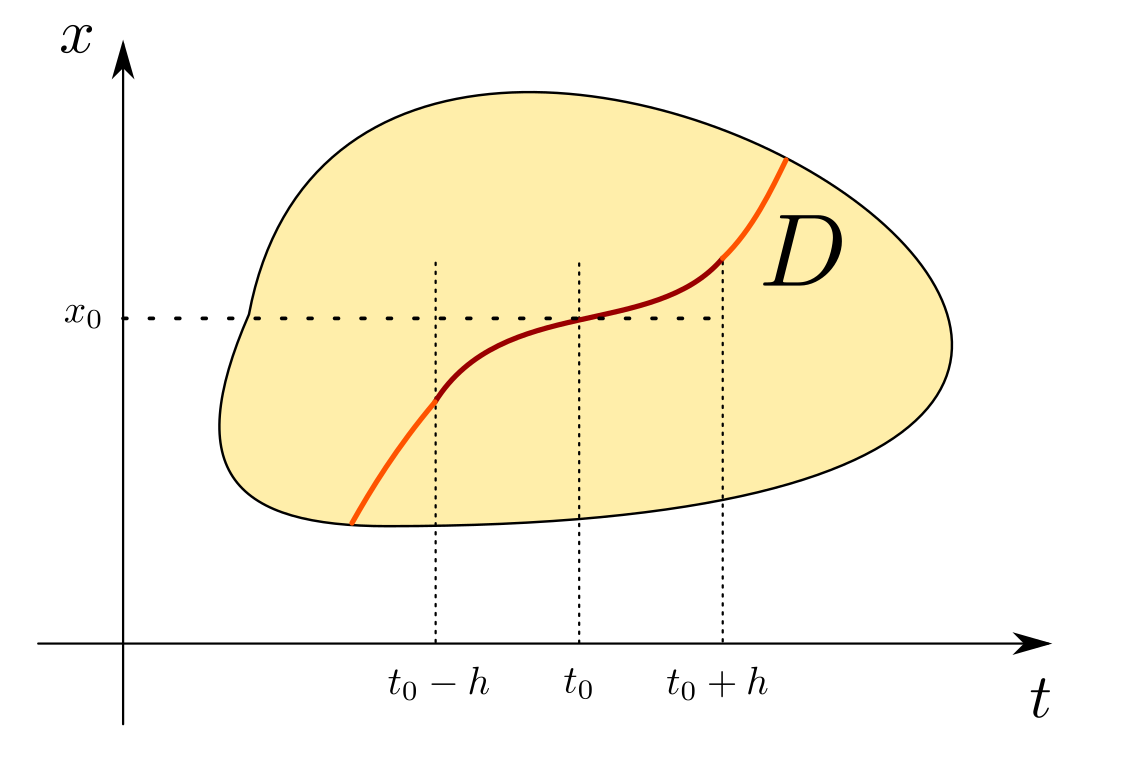
\includegraphics[scale=0.35]{assets/lect0.png} \end{center}
\end{boxteo}

\begin{boxteo}[Теорема Пікара]
  Нехай
  \begin{spacing}{1}
  \begin{enumerate}
    \item $\overrightarrow{f} \in C(\Pi)$;
    \item $\exists! L > 0 : \forall (t_1, \overrightarrow{x}_1), (t_2, \overrightarrow{x}_2) \in \Pi$ справедливо $|| f(t_1, \overrightarrow{x}_1) - f(t_2, \overrightarrow{x}_2)|| \leq \\ \leq L||\overrightarrow{x}_1 - \overrightarrow{x}_2||$ (умова Ліпшиця).
  \end{enumerate}
  \end{spacing}


  Тоді $\exists!$ розв'язок задачі Коші з початкової умови $\overrightarrow{x}(t_0) = \overrightarrow{x}_0(t)$, визначений принаймні на $I_h = (t_0 - h, t_0 + h), \  h = \min\{{a, \dfrac{b}{M}}\}, \  M = \max\limits_{\Pi}||f(t, \overrightarrow{x})||$.
\end{boxteo}

\subsection{Основні поняття теорії стійкості.}
Розглянемо систему диференційних рівнянь $\overrightarrow{x}' = \overrightarrow{f}(t, \overrightarrow{x})$ \eqref{nsde1}, де $f : D \rightarrow \mathbb{R}^n$ та $D = [a, +\infty) \times G, \quad G \subset \mathbb{R}^n$. Нехай при цьому $\overrightarrow{f}$ задавольняє умовам існування та єдиності розв'язку задачі Коші в будь-якій точці $(t_0, \overrightarrow{x}_0) \in D$

\bd
Розв'язок $\overrightarrow{x} = \overrightarrow{\varphi}(t)$ системи \eqref{nsde1} називається \textbf{стійким} за Ляпуновим, якщо

\begin{enumerate}
  \item $\overrightarrow{x} = \overrightarrow{\varphi}(t) \quad \exists  \text{ на } [a, +\infty)$ (відсутніть вертикальних асимптот)
  \item $\forall \varepsilon > 0 \quad \forall t_0 \geq a \quad \exists \delta > 0 : \forall $ розв'язку $\overrightarrow{x}(t)$ системи \eqref{nsde1} такого, що $||\overrightarrow{x}(t_0) - \overrightarrow{\varphi}(t_0)|| < \delta$ виконується наступне, що $\overrightarrow{x}(t)$ існує на $[t_0, +\infty)$ та $||\overrightarrow{x}(t) - \overrightarrow{\varphi}(t)|| < \varepsilon \quad \forall t \geq t_0$.
\end{enumerate}
\ed

\begin{center} 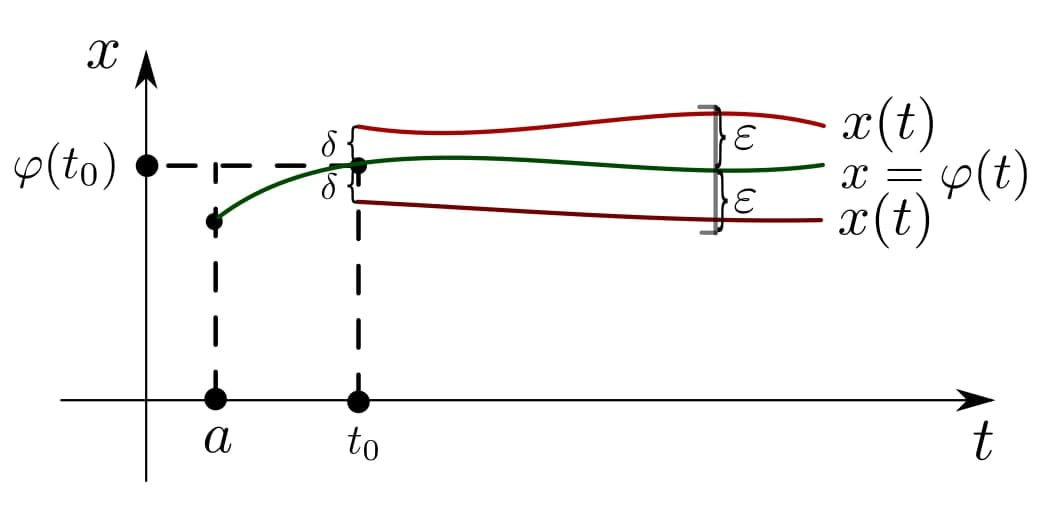
\includegraphics[scale=0.35]{assets/lect1.jpg} \end{center}

\bd
Розв'язок $\overrightarrow{x} = \overrightarrow{\varphi}(t)$ системи \eqref{nsde1} називається \textbf{асимптотично стійким} за Ляпуновим, якщо

\begin{enumerate}
  \item $\overrightarrow{x} = \overrightarrow{\varphi}(t)$ стійкий;
  \item $\forall t_0 \geq a \quad \exists \delta > 0: \forall$ розв'язку $\overrightarrow{x}(t)$ с-ми \eqref{nsde1} такого, що $||\overrightarrow{x}(t_0) - \overrightarrow{\varphi}(t_0)|| < \delta$ справедливо, що $||\overrightarrow{x}(t_0) - \overrightarrow{\varphi}(t_0)|| \rightarrow 0 \text{ при } t \rightarrow + \infty$.
\end{enumerate}

\begin{center} 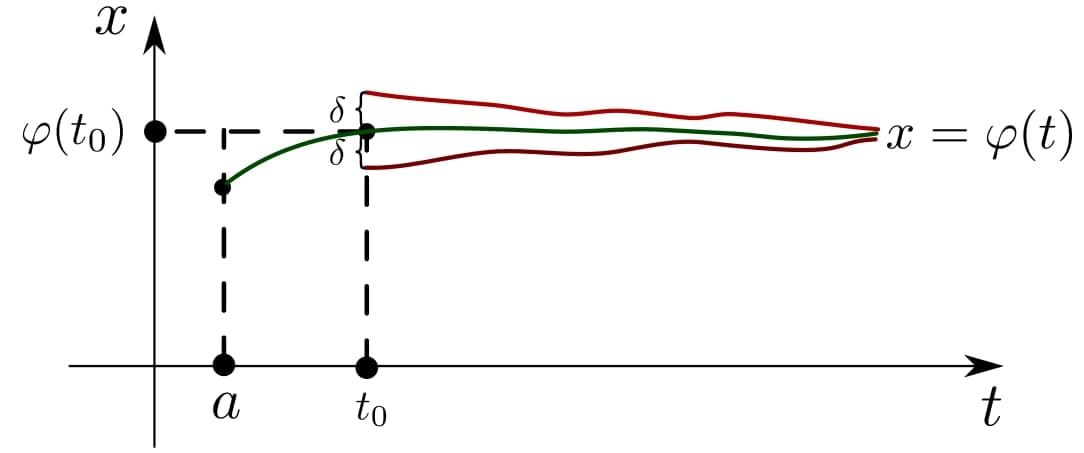
\includegraphics[scale=0.35]{assets/lect2.jpg} \end{center}

Роз'язок $\overrightarrow{\varphi}(t)$ називається \textbf{нестійким за Ляпуновим}, якщо він не є стійким, тобто:
\ed

\begin{enumerate}
  \item Або $\overrightarrow{x} = \overrightarrow{\varphi}(t) \quad \nexists$ на  $[a, +\infty)$ (вертикальні асимптоти);
  \item Або $\exists \varepsilon > 0 : \exists t_0 \geq a :  \forall \delta > 0$ існує розв'язок $\overrightarrow{x}(t)$ системи \eqref{nsde1} такий, що $||\overrightarrow{x}(t_0) - \overrightarrow{\varphi}(t_0)|| < \delta$, але $||\overrightarrow{x}(t_0) - \overrightarrow{\varphi}(t_0)|| > \varepsilon$
\end{enumerate}

\vfill
\begin{center} 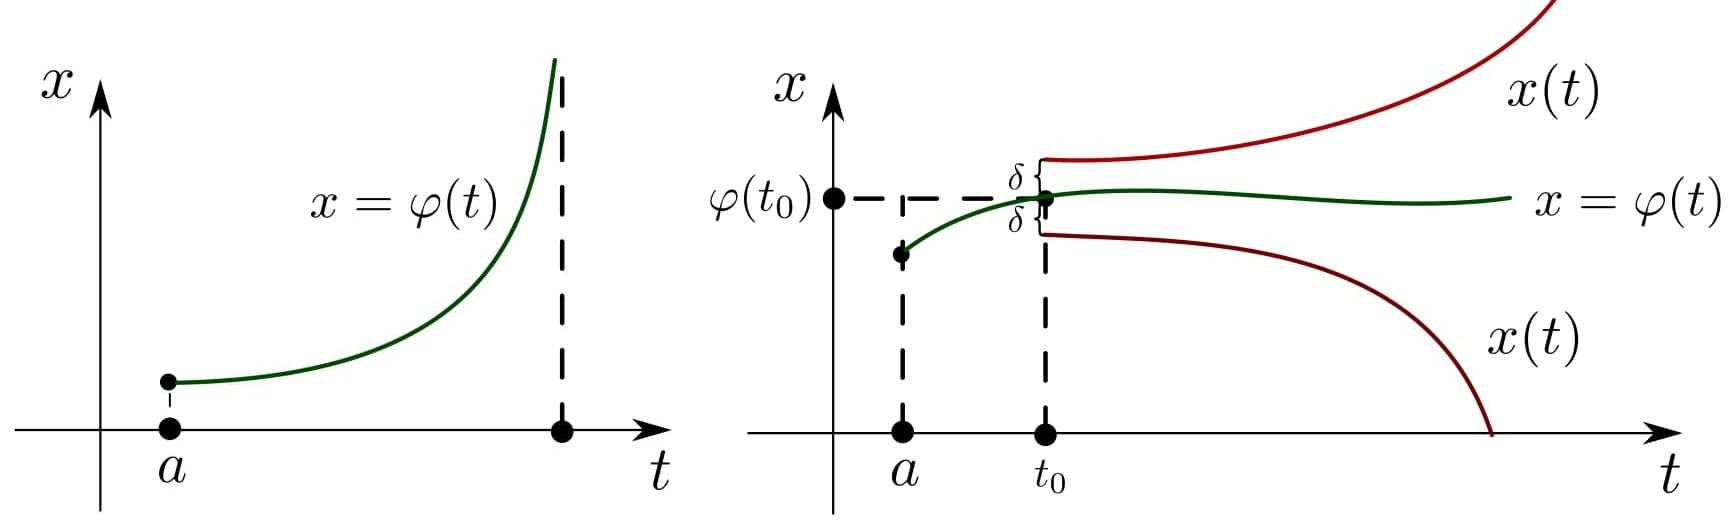
\includegraphics[scale=1.15]{assets/lect3+4.jpg} \end{center}
\vfill
\subsection{Приклади дослідження на стійкість за означенням.}

\begin{example}
    Дослідити на стійкість розв'язок задачі Коші:
$$
\begin{cases}
    x' = 1 \\
    x(0) = 0
\end{cases}
$$

\begin{enumerate}
\item Знайдемо розв'язок заданої задачі Коші: $x = 1 \Rightarrow x = t + C$ - загальний розв'язок. Підставимо: $ x(0) = 0 \quad \Rightarrow \quad 0 = 0 + C \quad \Rightarrow \quad C = 0 \quad \Rightarrow \quad$ \fbox{ $ \varphi(t) = t $} -- розв'язок, який будемо досліджувати.
Зазначений розв'язок не має вертикальних асимптот та $\exists$ на $\mathbb{R}$.

\item Знайдемо розв'язок довільної задачі Коші $x(t_0) = x_0$.
$$
x_0 = t_0 + C \quad \Rightarrow \quad C = x_0 - t_0 \quad \Rightarrow \quad x(t) = t + x_0 - t_0
$$
\item Нехай $  \left| x(t_0) - \varphi(t_0) \right|  =  \left| x_0 - t_0 \right| < \delta$, тоді $ \left| x (t) - \varphi (t) \right|  = \left|  x_0 - t_0 \right| < \varepsilon = \delta $.\\
Таким чином, розв'язок є стійким, але не є асимптотично стійким.

\end{enumerate}

\end{example}

\begin{example}
    Дослідити на стійкість розв'язок  задачі Коші:
    $$
    \begin{cases}
        x' = 1 + t - x \text{  -- лінійне неоднорідне рівняння першого порядку}\\
        x(0) = 0
    \end{cases}
    $$
    \begin{enumerate}

    \item Знайдемо розв'язок даної задачі Коші:
    $$
    x' = - x + 1 + t = \left| \begin{gathered}
     \text{ метод Бернуллі: } \\ x = uv
    \end{gathered}\right| = t + Ae^{-t}
    $$
    Знайшли загальний розв'язок. Із умови задачі Коші: $ A = 0 \Rightarrow \fbox {$\varphi(t) = t$ }$

    \item Знайдемо розв'язок довільної задачі Коші:
    $$
    x(t_0) = x_0, \quad x_0 = t_0 + Ae^{-t_0} \quad \Rightarrow \quad A = (x_0 - t_0) e^{t_0}
    $$
    Отримали: $x(t) = t + (x_0 - t_0) e^{t_0 - t} - \text{ загальний розв'язок задачі Коші}$

    \item Беремо $\left| x(t_0) - \varphi(t_0) \right| = |t_0 - x_0| < \delta$ і розглянемо:
    $$\left| x(t) - \varphi(t) \right| = |t - t - (x_0 - t_0)e^{t_0 - t}| < \delta e^{t_0 - t} \rightarrow 0, \text{ при } t \rightarrow + \infty$$
    Отже, $\forall t_0 \quad \exists \delta > 0 :$ для будь-якого розв'язку $x(t): |x(t_0) - \varphi(t_0)| = |x_0 - t_0| < \delta$ справедливо, що $|x(t) - \varphi(t)| \rightarrow 0 \text{ при } t \rightarrow + \infty$. Отримали, що розв'язок даної задачі Коші $\varphi(t) = t$ є асимптотично стійким.
    \end{enumerate}
\end{example}

\remark
Очевидно, що простіше досліджувати на стійкість розв'язок типу $\varphi(t) = 0$. Нехай \eqref{nsde1} $\overrightarrow{x}'(t) = \overrightarrow{f}(t, \overrightarrow{x})$, а $\overrightarrow{x} = \overrightarrow{\varphi(t)}$ -- розв'язок, який потрібно дослідити на стійкість. Застосуємо заміну: $\overrightarrow{z} = \overrightarrow{x} - \overrightarrow{\varphi}(t), \text{ де } \overrightarrow{z}$ -- нова невідома вектор-функція. Отримаємо систему:
$$
\overrightarrow{z}'(t) + \overrightarrow{\varphi}'(t) = \overrightarrow{f}(t, \overrightarrow{z} + \overrightarrow{\varphi}(t)) \quad \Rightarrow \quad \overrightarrow{z}'(t) = \overrightarrow{f}(t, \overrightarrow{z} + \overrightarrow{\varphi}(t)) - \overrightarrow{f}(t, \overrightarrow{\varphi})(t) \quad (*)
$$
Можно довести, що розв'язок $\overrightarrow{x} = \overrightarrow{\varphi}(t)$ системи \eqref{nsde1} -- стійкий (асимптотично стійкий або нестійкий) $\Longleftrightarrow$ розв'язок $\overrightarrow{z} = \overrightarrow{0}$  cистеми $(*)$ -- стійкий (асимптотично стійкий або нестійкий).

\subsection{Стійкість розв'язків лінійних систем}
Лінійна неоднорідна система рівнянь n-ого порядку має вигляд (далі ЛНС):
\be \label{srls1}
\overrightarrow{x}' = A(t) \overrightarrow{x} + \overrightarrow{f} (t).
\ee

$ \text{Де } A(t) \in \mathbb{R}^{n \times n}, \quad A(t) \in C [ a, + \infty), \quad \overrightarrow{f} \in C[a, + \infty)$ \\

Тоді $\forall t_0 \geq a, \quad \forall \overrightarrow{x}_0 \in \mathbb{R}^n \quad$ існує єдиний розв'язок ЛНС \eqref{srls1} з початковими умовми $\overrightarrow{x}(t_0) = \overrightarrow{x}_0$, визначений на $[a, +\infty)$.

Нехай $\overrightarrow{\varphi}(t)$ -- розв'язок \eqref{srls1}, який потрібно дослідити на стійкість.
Застосуємо заміну: $ \overrightarrow{z} (t) = \overrightarrow{x} - \vphi (t)$, де $ \overrightarrow{z}(t)$ - нова невідома вектор-функція, а $\vphi (t)$ - розв'язок, який ми маємо дослідити на стійкість.

Отримали лінійну однорідну систему першого порядку (далі ЛОС):

$$ \overrightarrow{z}'(t)   + \vphi'(t) = A(t)\overrightarrow{z}(t) + A(t)\vphi(t) + \overrightarrow{f}(t) $$
\be \label{losp1}
\overrightarrow{z}' = A(t) \overrightarrow{z} \text{ -- ЛОС n-ого порядку}
\ee

Заміною ми звели дослідження довільного розв'язку лінійної неоднорідної системи до дослідження нульового розв'язку відповідної ЛОС. Таким чином, приходимо до висновку, що усі розв'язки є одночасно стійкими, асимптотично стійкими або не стійкими. А отже, розглядаючи будь-яку лінійну систему, можемо говорити про стійкість не окремого розв'язку, а системи в цілому. Досліджуючи при цьому розв'язок $\overrightarrow{x}(t) = \overrightarrow{0}$\\

Розв'яжемо ЛОС \eqref{losp1} (перейдемо до змінної $x$): $\quad \overrightarrow{x}'  =  A(t) \overrightarrow{x} $ -- ЛОС \eqref{losp1}.

$X(t) $ -- її фундаментальна матриця (далі позначаємо ФМ). Тоді загальний розв'язок: $ \overrightarrow{x} (t) = X(t) \cdot \overrightarrow{C}$, де $\overrightarrow{ C} \in \mathbb{R}^n$.
Розв'язок задачі Коші з початковими умовами $ \overrightarrow{x} (t_0) = \overrightarrow{x_0}$:
$$
\overrightarrow{x}_0 = X(t_0) \cdot \overrightarrow{C} \Rightarrow \overrightarrow{C} = X^{-1} (t_0) \cdot \overrightarrow{x_0} \Rightarrow \fbox{$x(t) = X(t) X^{-1}(t_0) \overrightarrow{x}_0$}
$$

\begin{spacing}{2.5}
  \begin{boxteo}[Про стійкість ЛОС]\quad \\
  а) \eqref{losp1} - стійка $\Longleftrightarrow \exists K > 0: \sup\limits_{t\geq  a} ||X(t) || \leq K$.\\
  б) \eqref{losp1} - асимптотично стійка $\Longleftrightarrow  ||X(t)|| \to 0 $, при $ t \to +\infty$.\\
  в) \eqref{losp1} - нестійка. $ \Longleftrightarrow \exists \left\lbrace t_n \right\rbrace_{n=1}^{\infty} : ||X(t_n)|| \to +\infty $, при $n \to \infty$
  \end{boxteo}
\end{spacing}

\begin{spacing}{2.25}
\begin{proof}
а) \fbox{$\Longleftarrow$} \\ Нехай $ \exists K > 0 : \sup\limits_{t\geq a} ||X(t)|| \leq K$.

Доведемо стійкість розв'язку $\overrightarrow{x} (t) = \overrightarrow{0}.$ За означенням, візьмемо розв'язок довільної задачі Коші з початковими умовами $\overrightarrow{x } (t_0) = \overrightarrow{x}_0$.
Нехай $|| \overrightarrow{x}_0 || < \delta$ і розглянемо $ || \overrightarrow{x} (t)|| = || X(t) \cdot X^{-1} (t_0) \cdot \overrightarrow{x}_0 || \leq ||X(t)|| \cdot || X^{-1} (t_0)|| \cdot || \overrightarrow{x}_0|| \leq K \cdot || X^{-1} (t_0)|| \cdot || \overrightarrow{x}_0|| < K || X^{-1} (t_0)||\delta < \varepsilon $ при $ \delta = \dfrac{\varepsilon }{K || X^{-1} (t_0)|| + 1} $.
Отже, $\forall t_0 \geq  a \quad \forall \varepsilon >0 \quad \exists \delta > 0 \quad \left(  \delta = \dfrac{\varepsilon }{K || X^{-1} (t_0)|| + 1}  \right)$  для довільного розв'язку з $ || \overrightarrow{x}_0|| < \delta$ справедливо $ ||\overrightarrow{x} (t)|| < \varepsilon  \quad \Longrightarrow \quad $ стійкість розв'язку.
\end{proof}
\end{spacing}
\begin{proof}
a) \fbox{$\Longrightarrow$} \\ Нехай \eqref{losp1} - стійка. Припустимо від супротивного, що

$$\exists  \left\lbrace t_n \right\rbrace_{n\geq 1}^{\infty} : t_n \rightarrow +\infty : ||X(t_n)|| \to {+\infty} \text{ при } n \to \infty$$\\
Тоді $\exists j = \overrightarrow{1, n} : || \overrightarrow{x}^{j} (t_n)|| \to \infty$, де $\overrightarrow{x}^j$  - це $j$-тий стовпчик ФМ. \\ Покладемо $\forall \delta > 0:$


$$
\overrightarrow{x}^{\delta}_0 = \frac{\delta X(t_0) \overrightarrow{e}_j}{2 ||X(t_0)||} \text{ , де }\overrightarrow{e}_j = \begin{bmatrix}
0\\
\vdots\\
1\\
\vdots\\
0
\end{bmatrix} - j
$$

Тоді $|| \overrightarrow{x}_0^{\delta}|| = \dfrac{1}{ 2 ||X(t_0)||}  \cdot \delta ||X(t_0) \cdot \overrightarrow{e}_j|| < \delta $.\\
Розглядаємо розв'язок задачі Коші з початковими умовами $ \overrightarrow{x} (t_0) = \overrightarrow{x} _0 ^ \delta$. Маємо:
$$
\overrightarrow{x} (t) = X(t) \cdot X^{-1}(t_0) \cdot \overrightarrow{x}_0 ^\delta = X(t) X^{-1} (t_0) \cdot \dfrac{ \delta X(t_0) \overrightarrow{e}_j}{ 2 ||X(t_0)||} = \frac{\delta}{2} \cdot \frac{X(t) \overrightarrow{e}_j}{ ||X(t_0)||} = \frac{\delta}{2 ||X(t_0)|| } \cdot \overrightarrow{x}^j (t)
$$
$$
\Longrightarrow \forall \varepsilon >0 \quad \exists n_0 \in \mathbb{N} \quad : \forall n \geq n_0
$$
$$
||\overrightarrow{x} (t_n)|| = \frac{\delta}{ 2 ||X(t_0)|| } \cdot ||\overrightarrow{x}^j (t_n)|| \to \infty > \varepsilon
$$
Отримали нестійкість системи $ \Rightarrow  $ суперечність початковій побудові $ \Rightarrow$ a).\\
Пункт б) доводиться аналогічно а). $\quad$ Пункт в) випливає із пукнта а).
\end{proof}

\subsection{Стійкість ЛОС зі сталою матрицею.}

\begin{equation}\label{slsm2}
\overrightarrow{x} ' (t) = A \overrightarrow{x} (t) \text{, де $A$ - стала матриця $n \times n$}
\end{equation}
\begin{boxteo} \quad \\
a) \eqref{slsm2} - стійка $ \Longleftrightarrow  \forall \lambda $ - власне число матриці $A$: \\
$\Re \lambda \leq 0$, причому якщо $ \Re \lambda = 0$, то йому відповідають лише одновимірні клітини Жордана. \\
б) \eqref{slsm2} - асимптотично стійка $ \Longleftrightarrow \forall \lambda $ - власні числа матриці $A: \Re \lambda < 0 $.\\
в) \eqref{slsm2} - нестійка $ \Longleftrightarrow $ не є стійкою.
\end{boxteo}

\begin{proof}
Нехай $ \lambda = \alpha + i\beta$ - власне число матриці $A \Rightarrow $ у ФМ цьому власному числу відповідає розв'язок: \\
 - якщо $ \lambda$ відповідають лише одновимірні клітини Жордана:
 $$
 \overrightarrow{x} (t) = e^{\alpha t} ( \overrightarrow{Q} _0 \cos{(\beta t)} + \overrightarrow{R}_0 \sin{(\beta t)} )
$$
- якщо клітина Жордана розміру $l$:
$$
\overrightarrow{x} (t) = e^{\alpha t} ( \overrightarrow{Q} _{l-1} \cos{(\beta t)} + \overrightarrow{R}_{l-1} \sin{(\beta t)} )
$$
Тоді:\\
якщо $ \Re \lambda = \alpha < 0  \Rightarrow || \overrightarrow{x} (t)|| \to 0 $ за $t \to \infty$.\\
якщо $ \Re \lambda = \alpha >0 \Rightarrow || \overrightarrow{x} (t)|| \to + \infty $ за $t \to \infty$.\\
якщо $ \Re \lambda = 0 $, то:\\
\hspace*{1cm} - якщо лише одновимірні клітини Жордана: $||\overrightarrow{x}(t) ||$ - обмежена.\\
\hspace*{1cm} - якщо клітини Жордана розмірності $l \geq 2$ : $ || \overrightarrow{x} (t)|| \to + \infty $ за $t \to \infty. $
\end{proof}
\begin{example}
    $$\begin{cases}
        x' = 3x + y \\
        y' = y-x
    \end{cases} \qquad \qquad A = \begin{bmatrix}
     3 & 1 \\ -1 & 1
    \end{bmatrix}
    $$
    $$
    \det \left( A - \lambda I  \right) = \begin{vmatrix}
      3 - \lambda & 1 \\
      -1 & 1- \lambda
    \end{vmatrix}  = (3 - \lambda) (1- \lambda) + 1 = \lambda^2 - 4 \lambda + 3 = (\lambda-2 )^2
    $$
    Отримали дійсне власне число $\lambda=2$, кратності 2. $ \Re \lambda = 2 > 0 \Rightarrow $ Система нестійка.
\end{example}
\textbf{Зауваження.} Перевірку умов теореми в частині, що стосується стійкості, можна здійснювати нне знаходячи власних чисел матриці $A$.

\begin{spacing}{1.25}
  \begin{boxteo}[Критерій Рауса-Гурвіца]
  $$
  \det \left( A - \lambda I \right) = a_0 \lambda^n + a_1 \lambda^{n-1} + ... + a_n ; \quad a_1 \in \mathbb{R}, a_0 > 0;
  $$
  $
  \Re \lambda < 0 \quad \forall \lambda \quad \Longleftrightarrow \quad
  $ всі головні мінори матриці Гурвіца $H$ додатні, де $ H =  \left( h_{ij} \right)^n_{ij=1} $
  $$
  h_{ij} = \begin{cases}
      a_{2i-j}, & 0 \leq 2i - j \leq  n;\\
      0 , & \text{інакше.}
  \end{cases}
  $$
  \end{boxteo}
\end{spacing}

\section{Лекція 2}
\subsection{Приклади дослідження на стійкість диф. рівнянь, що описують поведінку екологічних процесів.}

\subsubsection{Модель одновимірної популяції.}
Однією з важливих проблем екології є динаміка чисельності популяції. Нехай маємо популяцію, що складається з особин одного виду, знайдемо закон зміни її чисельності. \\

Припустимо, що існують лише процеси розмноження та смерті, швидкості яких пропорційні кількості особин в даний момент часу; не враховується внутрішньовидова боротьба; розглядаємо лише одну популяцію (відсутність хижаків). \\

$x(t) - $ кількість особин в момент $t$, $\quad R$ -- швидкість розмноження. \\
$\gamma - $ коефіцієнт розмноження, $\quad R = \gamma x $.\\
$ S - $ швидкість природньої загибелі, $\sigma - $ коефіцієнт смертності (природньої).\\
$S = - \sigma x$, тоді: $ \dfrac{\mathrm{d}x}{\mathrm{d}t} = \gamma x - \sigma x = (\gamma - \sigma)x $.\\

Позначення: $ \gamma - \sigma = a$.

$$
\text{Тоді: $\quad$ \fbox{$\dfrac{\mathrm{d}x}{\mathrm{d}t} = ax $} -- закон Мальтуса.}
$$
\begin{center} 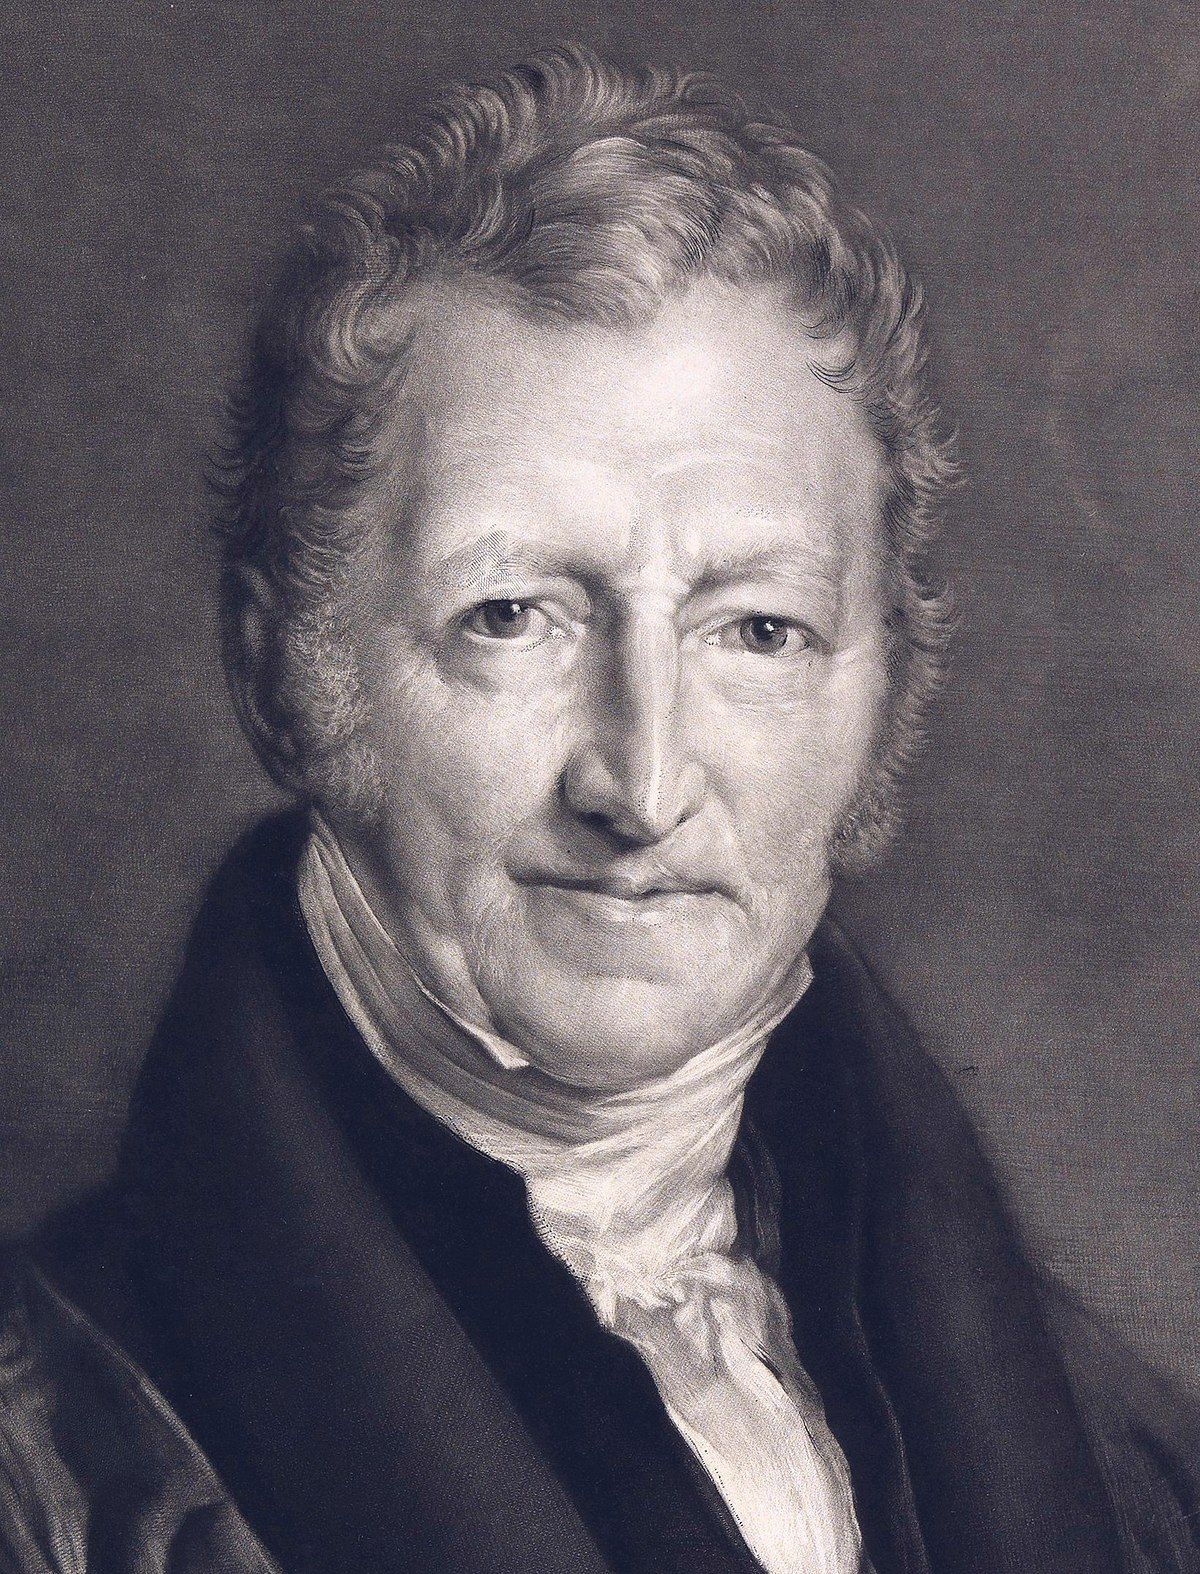
\includegraphics[scale=0.2]{assets/lectures_recent-44a47cac.png} \end{center}

Томас Мальтус (1766-1834), -- англійский вчений, демограф, економіст, священик; робота 1798 року: ''Все про принципи народонаселення''.
$$
\dfrac{\mathrm{d}x}{\mathrm{d}t} = ax \Longrightarrow x(t) = C \cdot e^{at} \text{ -- загальний розв'язок.}
$$
Нехай в початковий момент часу $t_0 = 0$ кількість особин складає $x_0$ особин:
$$
x(0) = x_0
$$
Тоді: $x(t) = x_0 \cdot e^{at} $ -- розв'язок даної задачі Коші. Розглянемо випадки:

\begin{enumerate}
  \item $a < 0$ (помирають більше, ніж народжується). Оскільки дане рівняння є лінійним, то всі розв'язки водночас стійкі (нестійкі, асимптотично стійкі). Тому дослідимо на стійкість розв'язок $ \varphi(t) = 0$ (умова 1. стійкості виконується); розв'язок довільної задачі Коші:
  $$
  x(t_0) = x_0 \quad : \quad x(t) = x_0 e^{a (t-t_0)}
  $$
  Нехай $ \left| x_0 \right| < \delta.$ Розглянемо:
  $$
  \forall t \geq t_0 \quad \left| x (t) \right| = \underbrace{e^{a(t-t_0)}}_{<1, \text{ при } t\geq t_0} \left| x_0 \right| \xrightarrow[t\to + \infty]{} 0 < \varepsilon \text{ при } \varepsilon = \delta
  $$
  $\Rightarrow $ всі розв'язки рівняння асимптотично стійкі та прямують до нуля.\\
  \begin{center} 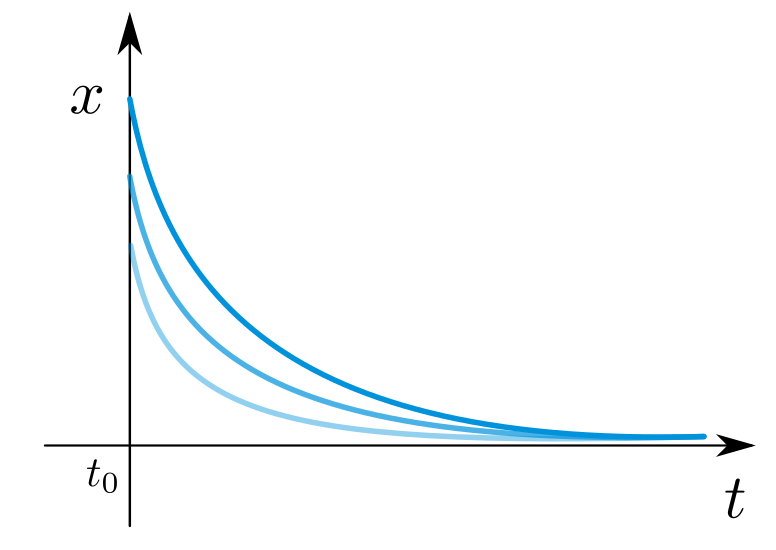
\includegraphics[scale=0.33]{assets/lectures_recent-562c17da.png} \end{center}
  Це означає, що якою б великою не була кількість особин в початковий момент часу, якщо смертність перевищує народжуваність, кількість особин з часом прямує до 0 ($t \to + \infty$).

  \item a = 0 (смертність = народжуваність). В цьому випадку розв'язок задачі Коші:
  $$ x(t_0) = x_0 \quad : \quad x(t) = x_ 0 $$
  Відповідно при $|x_0| < \delta$ маємо $|x(t)| = |x_0| < \varepsilon = \delta$. Отримали стійкість, але не асимптотичну.
  \begin{center}
    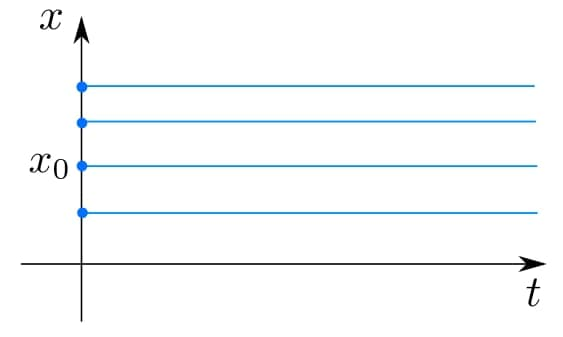
\includegraphics[scale=0.65]{assets/bcase.jpg}
  \end{center}
  Чисельність особин є сталою в кожний момент часу, коли смертність співпадає з народжуваністю.

  \item a > 0 (смертність < народжуваність). Візьмемо $\varphi(t) = 0$, розв'язок для будбудь-якої задачі Коші:
  $$ x(t_0) = x_0e^{a(t-t_0)}$$
  Нехай $|x_0| < \delta$
  $$\forall t \geq t_0 \quad |x(t)| = e^{a(t-t_0)}|x_0| \rightarrow +\infty \quad \text{ при } \quad t \rightarrow +\infty$$
  Отже,
  $$\exists \varepsilon > 0 \quad \exists t_0 \geq 0 : \forall \delta > 0$$ для розв'язку $x(t)$ з початковими умовами $x(t_0) = x_0 : |x(t_0)| < \delta$, але $|x(t)| > \varepsilon$, починаючи з деякого моменту (нестійкість)
  \begin{center}
    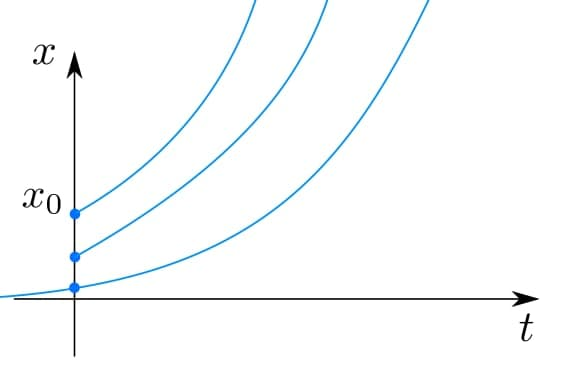
\includegraphics[scale=0.65]{assets/vcase.jpg}
  \end{center}
  В даному випадку чисельність особин необмежено, експоненційно зростає з часом і $\rightarrow +\infty$ при $t \rightarrow +\infty$, розв'язки рівняння нестійкі.
\end{enumerate}

\subsubsection{Модель Ферхюльста (логістична модель)}
\begin{center}
  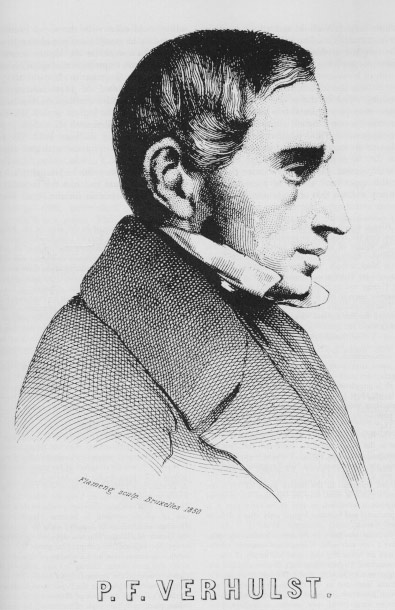
\includegraphics[scale=0.6]{assets/verhulst.jpg}
\end{center}

Нехай між особинами є внутрішньовидова боротьба, що додає додаткове джерело загибелі. Отже смертність:
\begin{enumerate}
  \item природна:  $-\sigma x$;
  \item внутрішньовидова боротьба: $- \mu x^2$.
\end{enumerate}

Швидкість народжуваності: $R = \gamma x$.  Швидкість смертності: $S = - \sigma x - \mu x^2$.\\
$$
\dfrac{\mathrm{d}x}{\mathrm{d}t}  = \gamma x -  \sigma x - \mu x^2 = \underbrace{(\gamma - \sigma)}_{=аеa}x - \mu x^2
$$

\begin{center}
    \fbox{$ \dfrac{\mathrm{d}x}{\mathrm{d}t} = ax - \mu x^2 $} -- закон Ферхюльста.
\end{center}
Розглянемо $a > 0$, тобто народжуваність більше смертності.
\begin{center}
  Зауважимо, що $ax - \mu x^2 = x ( a - \mu x)$.
\end{center}

Проаналізувавши праву частину, бачимо, що:
\begin{itemize}
  \item $\dfrac{\mathrm{d}x}{\mathrm{d}t} > 0 (\uparrow) \text{ при } x \in (0, \dfrac{a}{\mu})$
  \item $\dfrac{\mathrm{d}x}{\mathrm{d}t} < 0 (\downarrow) \text{ при } x \in (- \infty, 0) \cup ( \dfrac{a}{\mu}, +\infty)$
  \item $\dfrac{\mathrm{d}x}{\mathrm{d}t} = 0 \text{ при } x = 0 \lor x = \dfrac{a}{\mu}$
\end{itemize}

\begin{center} 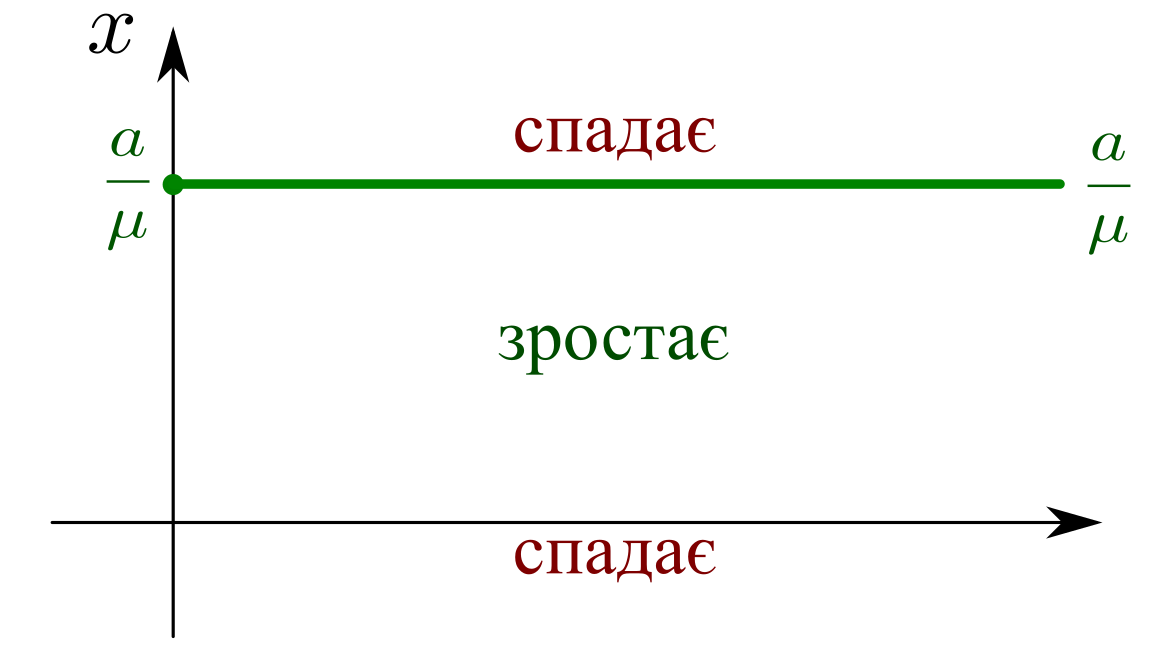
\includegraphics[scale=0.28]{assets/lectures_recent-e4b7cd02.png} \end{center}

Розв'яжемо рівняння: $\dfrac{\mathrm{d}x}{\mathrm{d}t} = ax - \mu x^2 $ -- рівняння Бернуллі.
\begin{spacing}{2}
  $x = u\cdot v $, $ \quad u'v + v'u - auv = - \mu u^2 v^2 $, $\quad u'v + u(v' - av) = - \mu u^2 v^2 $\\
  $v' = av$, $\quad \dfrac{\mathrm{d}v}{v} = a\mathrm{d}t \quad \Longrightarrow \quad v = e^{at}$, $\quad u' =- \mu u^2 v$, $\quad \dfrac{\mathrm{d}u}{u^2} = - \mu e^{at}\mathrm{d}t $\\
  Тоді: $ -\dfrac{1}{u} = -\dfrac{ \mu}{a}e^{at} - C $, звідси отримуємо:\\
  $ u = \dfrac{1}{ \frac{u}{a} e^{at} +c } = \dfrac{a}{ \mu e^{at} + aC} \quad \Longrightarrow \quad x = uv = \dfrac{a e^{at}}{ \mu e^{at} + aC  }  =  \dfrac{a}{ \mu  + aCe^{-at}}  $\\ \\
  Загальний розв'язок:
  $\left[ \begin{gathered}
   x= \frac{a}{ \mu  + aCe^{-at}}\\
   x = 0
  \end{gathered} \right.$
\end{spacing}


Знайдемо довільний розв'язок задачі Коші: $x(t_0) = x_0: \quad x_0 = \dfrac{a}{\mu + aCe^{-at_0}}$\\
$\mu + aC\cdot e^{-at_0} = \dfrac{a}{x_0}, \quad C = \dfrac{\left( \dfrac{a}{x_0} - \mu  \right)\cdot e^{at_0} }{a} = \dfrac{a - \mu x_0}{ax_0}\cdot e^{at_0} \Longrightarrow$
$$
\Longrightarrow x(t) = \dfrac{a}{ \mu + \frac{a - \mu x_0}{x_0} \cdot e^{a(t_0 - t)} } = \dfrac{ax_0}{ \mu x_0 - (a - \mu x_0 ) \cdot e^{a(t_0-t)}}
$$

Отримали розв'язок $ \varphi (t) = \dfrac{a}{\mu} \quad \exists $  на $[0, + \infty)$.
\begin{spacing}{3}
  Перевіримо другу умову стійкості. Візьмемо $ \left| x - \dfrac{a}{\mu} \right| = \left| \dfrac{\mu x_0 - a}{\mu}  \right| < \delta $
  \\ і розглянемо: $
  \left| x(t) - \varphi(t) \right| = \left| \dfrac{ax_0}{\mu x_0 - (a - \mu x_0) \cdot e^{a (t_0 - t)}}  - \dfrac{a}{ \mu}  \right| = \\ \left| \dfrac{a\mu x_0 - a\mu x_0 + a (a - \mu x_0 )\cdot e^{a(t_0 - t)}}{\mu (\mu x_0 - (a- \mu x_0)\cdot e^{a(t_0 -t)})}  \right| = \dfrac{a (a - \mu x_0)\cdot e^{a (t_0 - t)}}{ \mu^2 x_0 - \mu (a- \mu x_0) \cdot e^{a(t_0 - t)}} \xrightarrow[t\to +\infty]{} 0$
\end{spacing}


Таким чином, розв'язок $\varphi(t) = \frac{a}{\mu}$ - асимптотично стійкий.
\begin{center} 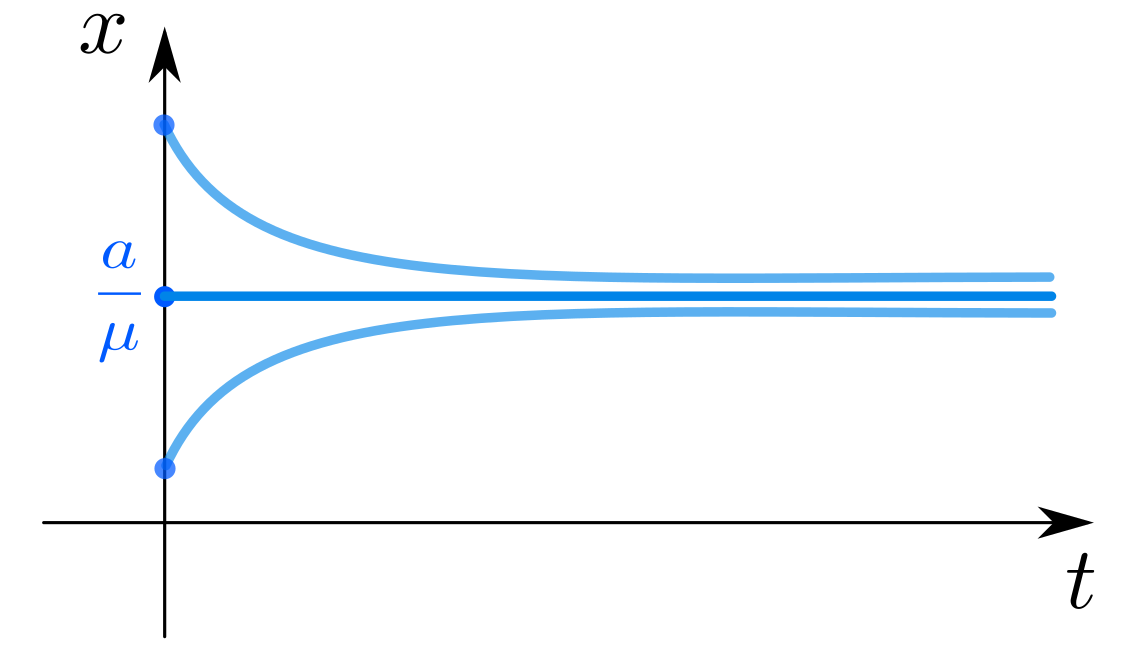
\includegraphics[scale=0.3]{assets/lectures_recent-0b98e3f0.png} \end{center}
\begin{remark}
    1. Аналогічно можна показати, що $\varphi (t) = 0$ - нестійкий. Таким чином, внутрішньовидова боротба виступає ''природнім стабілізатором'' моделі одновимірної популяції. На відміну від моделі Мальтуса, де у випадку $ a > 0$ маємо нестійкість і нескінчений ріст популяції, в моделі Ферхюльста розв'язки стабілізуються в околі стлого розв'язку $\varphi(t) = \dfrac{a}{\mu}.$ Відзначимо також, що чим меньше значення $\mu$, тим швидше зростає чисельність особин.
\end{remark}
\begin{remark}
    2. При $ a\leq 0$ (смертність $\geq$  народжуваність) легко встановити, що $ x=0 $ -- асимптотично стійкий розв'язок.
\end{remark}

\subsection{Класифікація фазових портретів в околі положень рівноваги ЛОС 2-го порядку.}

\begin{defo}
    Положенням рівноваги нормальної системи диф. рівнянь:
    $$
    \begin{dcases}
        \dot{x_1} = f_1(x_1, ..., x_n)\\
        \qquad \quad \cdots\\
        \dot{x_n} = f_n(x_1, ..., x_n)
    \end{dcases}
    $$
    називається т. $\overrightarrow{x} = (x_1, ... , x_n)$ така, що:
    $$
    f_1 (\overrightarrow{x}) = f_2(\overrightarrow{x}) = \cdots = f_n(\overrightarrow{x}) =0
    $$
\end{defo}
Розглянемо ЛОС (1):$ \begin{cases}
    \dot{x} = ax + by\\
    \dot{y} = cx + dy
\end{cases}$, $\quad$ де a, b, c, d $\in \mathbb{R}, \quad A = \begin{bmatrix}
 a & b\\
 c & d
\end{bmatrix}$.\\


Нехай $\det A \neq 0$. Тоді єдине положення рівноваги системи (1) -- це точка (0,0).
\begin{defo}
    Фазовою траєкторією ЛОС (1) називається проекція її інтегральних кривих на площину $xOy$. Зображення фазових траєкторій на площині $xOy$ називають фазовим портретом.
\end{defo}
\textbf{Завдання.} Дослідити фазовий портрет ЛОС (1) в околі т. (0, 0), яка є її положенням рівноваги. Виявляється, що фазовий портрет ЛОС (1) в околі точки (0, 0) повністю визначається власними числами матриці $A$. Нехай $J(A)$ -- ЖНФ матриці $A$; $H$ - матриця переходу. \\

1. Нехай $\lambda_1 , \lambda_2 \in \mathbb{R} \quad \lambda_1 \neq \lambda_2 \quad \lambda_1 \cdot \lambda_2 > 0.$ \\ Для зручності здійснимо в системі (1):

$$
\begin{bmatrix}
 \dot{x}\\
 \dot{y}
\end{bmatrix} = A \begin{bmatrix}
 x \\
 y
\end{bmatrix} \text{ заміну: } \begin{bmatrix}
 x\\
 y
\end{bmatrix} = H \begin{bmatrix}
 u \\ v
\end{bmatrix} \text{, де }
 \begin{bmatrix}
 u \\
 v
\end{bmatrix} \text{ -- нова невідома вектор-функція}
$$

$$
H \begin{bmatrix}
 \dot{u}\\
 \dot{v}
\end{bmatrix} = A H  \begin{bmatrix}
 u \\
 v
\end{bmatrix} \quad \text{домножимо зліва на } H^{-1} \text{, тоді: }
H^{-1} H \begin{bmatrix}
\dot{u}\\
\dot{v}
\end{bmatrix}  =H^{-1} A H \begin{bmatrix}
 u \\
 v
\end{bmatrix}
$$

$$ \text{Таким чином, ми перейшли до Жарданового базису: }
\begin{bmatrix}
\dot{u}\\
\dot{v}
\end{bmatrix}  =J(A) \cdot \begin{bmatrix}
 u \\
 v
\end{bmatrix}
$$

\begin{spacing}{2}
\text{Маємо: } $
\begin{bmatrix}
\dot{u}\\
\dot{v}
\end{bmatrix} = \begin{bmatrix}
 \lambda_1 & 0 \\
 0 & \lambda_2
\end{bmatrix} \begin{bmatrix}
 u \\
 v
\end{bmatrix}
\left[ \begin{array}{l}
    \dfrac{dv}{du} = \dfrac{\lambda_2}{\lambda_1} \cdot \dfrac{u}{v}\\
    u = 0
\end{array} \right.
\Longleftarrow
\begin{cases}
    \dot{u} = \lambda_1 u \\
    \dot{v} = \lambda_2 v
\end{cases} \Longrightarrow
\begin{cases}
    u = c_1 \cdot e^{\lambda_1 t}\\
    v = c_2 \cdot e^{\lambda_2 t}
\end{cases} \\
$
\\ Поділили двуге рівняння на перше, щоб вилучити $t$.
\end{spacing}
$$
\left[ \begin{array}{l}
    \dfrac{dv}{du} = \dfrac{\lambda_2}{\lambda_1} \cdot \dfrac{u}{v}\\
    u = 0
\end{array} \right. \Longrightarrow \left[ \begin{array}{l}
    \ln{ \left| v \right| } = \dfrac{\lambda_2}{\lambda_1} \ln{ \left| u \right| } + \ln{ \left| c \right| } \\
    u = 0, v = 0
\end{array} \right. \Longrightarrow
\left[ \begin{array}{l}
    v = c  \cdot u^{ \frac{\lambda_2}{\lambda_1} }\\
    u = 0, v = 0
\end{array} \right.
$$
\\
Якщо $ \lambda_1 \cdot \lambda_1 > 0 $ та $ \left| \lambda_2 \right| > \left| \lambda_1 \right|  $ (стрілки від нуля за умови $
 \lambda_1, \lambda_2 > 0$):

\begin{center} 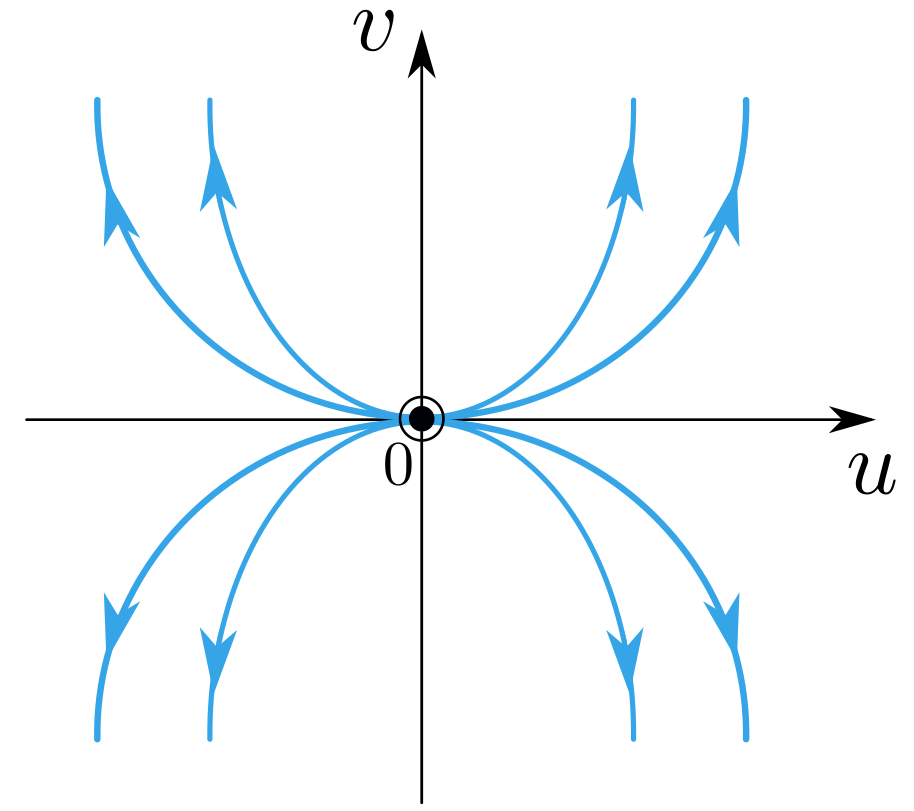
\includegraphics[scale=0.37]{assets/lectures_recent-b13d607a.png} \end{center}

Якщо $ \lambda_2 \cdot \lambda_1 > 0$ та  $ \left| \lambda_2 \right| > \left| \lambda_1 \right|  $ (стрілки до нуля за умови $
 \lambda_1, \lambda_2 < 0$):

 \begin{center} 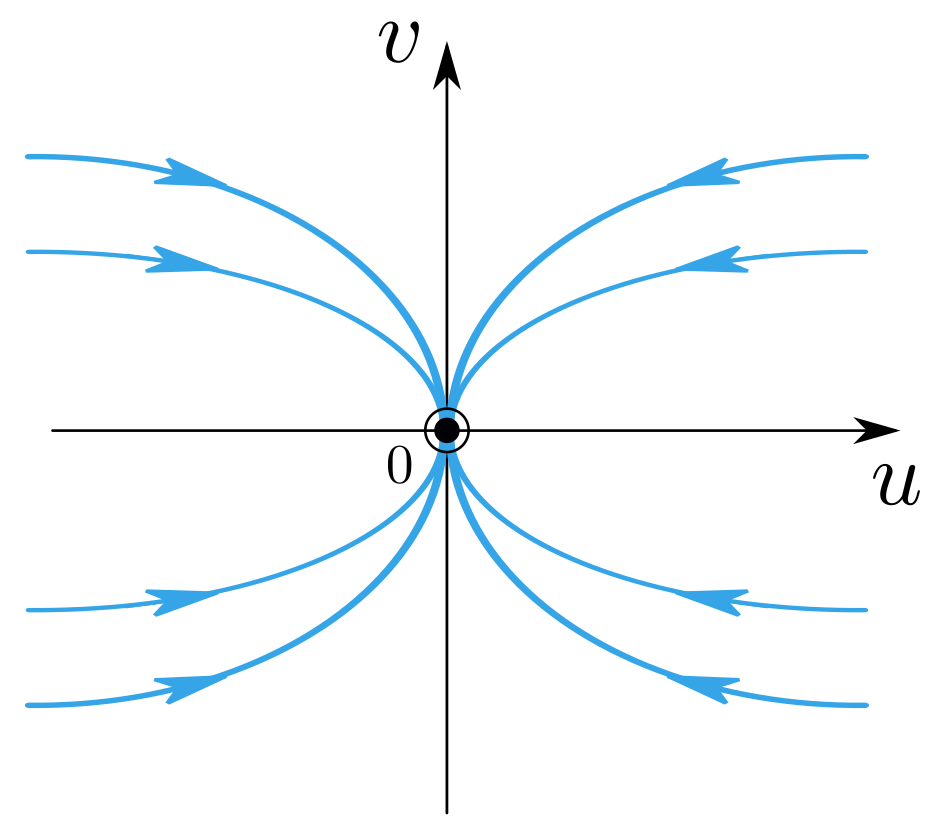
\includegraphics[scale=0.37]{assets/lectures_recent-392ff5ad.png} \end{center}

 Відмітимо, що якщо $\lambda_1, \lambda_2 < 0$, то напрям руху (по $t$) вздовж траєкторій відбувається до нуля. Якщо ж $\lambda_1, \lambda_2 >0$, то рух спрямовано від нуля.\\

 Залишається перейти до початкових змінних $ \begin{bmatrix}
  x \\
   y
 \end{bmatrix}$.\\
Таким чином, якщо $\lambda_1 , \lambda_2 \in \mathbb{R}, \lambda_1 \neq \lambda_2, \quad \lambda_1 \cdot \lambda_2 > 0$ (власні числа одного знаку), то фазовий портрет має вигляд:

\begin{center} 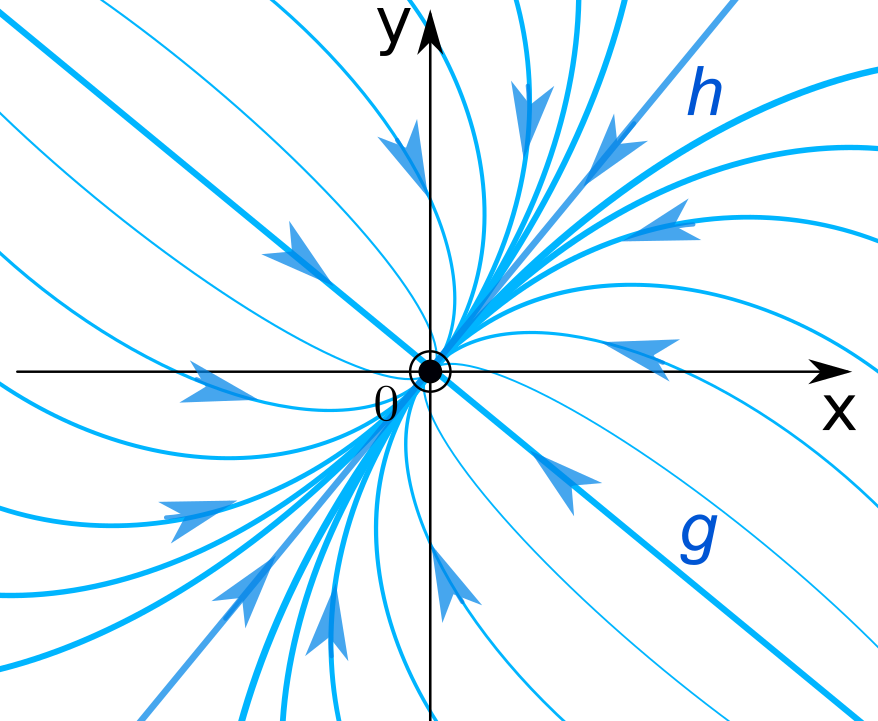
\includegraphics[scale=0.37]{assets/lectures_recent-deaf1762.png} \end{center}

На малюнку $h$ - пряма на якій лежить власний вектор, який відповідає меншому за модулем власному числу.\\
Такий фазовий портрет \textbf{вузол.}\\
- Якщо $\lambda_1, \lambda_2 > 0$ - нестійкий вузол (стрілки від нуля).\\
- Якщо $\lambda_1, \lambda_2 < 0$ - асимптотично стійкий вузол (стрілки до нуля). \\

\begin{example}
    $$
    \begin{cases}
    \dot{x} = 2y - 3x\\
    \dot{y} = x - 4y
    \end{cases} \qquad A = \begin{bmatrix}
     -3 & 2 \\
     1 & -4
    \end{bmatrix}
    $$
    $$
    \det{A - \lambda I} = \begin{vmatrix}
      -3 - \lambda & 2 \\
      1 & -4 - \lambda
    \end{vmatrix}  = (-3-\lambda) (-4 - \lambda) -2 = \lambda^2 + 7 \lambda + 10 = 0
    $$
    $$
    \lambda_1 = -2 \qquad \lambda_2 = -5 \quad \Longrightarrow \quad \text{асимптотично стійкий вузол.}
    $$
    Знаходимо власні вектори:\\
    $\lambda_1 = -2$:
    $$
    \begin{bmatrix}
     -1 & 2 \\
     1 & -2
    \end{bmatrix} \begin{bmatrix}
     h_1 \\
     h_2
    \end{bmatrix} = \begin{bmatrix}
     0 \\
     0
    \end{bmatrix} \qquad \begin{gathered}
     -h_1 + 2h_2 = 0\\
     h_1 = 2 h_2
    \end{gathered} \Rightarrow \overrightarrow{h} = \begin{bmatrix}
     2 \\
     1
    \end{bmatrix}
    $$
    $\lambda_2 = -5$
    $$
    \begin{bmatrix}
     2 & 2 \\
     1 & 1
    \end{bmatrix} \begin{bmatrix}
     g_1 \\
     g_2
    \end{bmatrix} = \begin{bmatrix}
     0 \\
     0
    \end{bmatrix}
    \qquad \begin{gathered}
     g_1 + g_2 = 0\\
     g_1 = - g_2
    \end{gathered} \Rightarrow \overrightarrow{g} = \begin{bmatrix}
     1 \\
     -1
    \end{bmatrix}
    $$

    \begin{center} 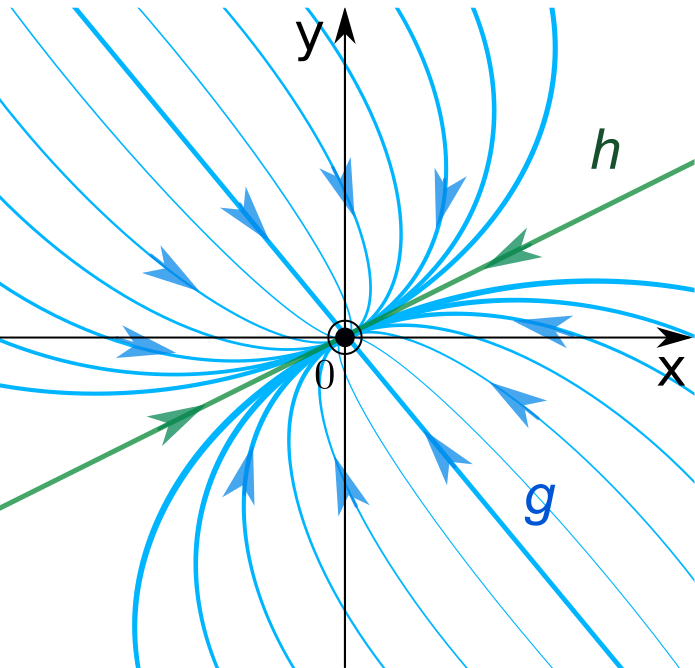
\includegraphics[scale=0.5]{assets/lectures_recent-06adae22.png} \end{center}
\end{example}

2. Нехай $ \lambda_1 , \lambda_2 \in \mathbb{R}, \lambda_1 \neq \lambda_2, \lambda_1 \cdot \lambda_2 < 0$ (Власні числа різних знаків).
Тоді, аналогічно, перейшовши до Жорданового базису, маємо:

$$
\begin{gathered}
\begin{cases}
    \dot{u} = \lambda_1 u\\
    \dot{v} = \lambda_2 v
\end{cases} \\ \begin{cases}
    u = c_1 \cdot e^{\lambda_1 t}\\
    v = c_2 \cdot e^{\lambda_2 t}
\end{cases} \\
 \left[ \begin{array}{l}
v = C \cdot u^{ \frac{\lambda_2}{\lambda_1} }\\
u =0 , v = 0
\end{array} \right.
\end{gathered}\quad
\begin{gathered} 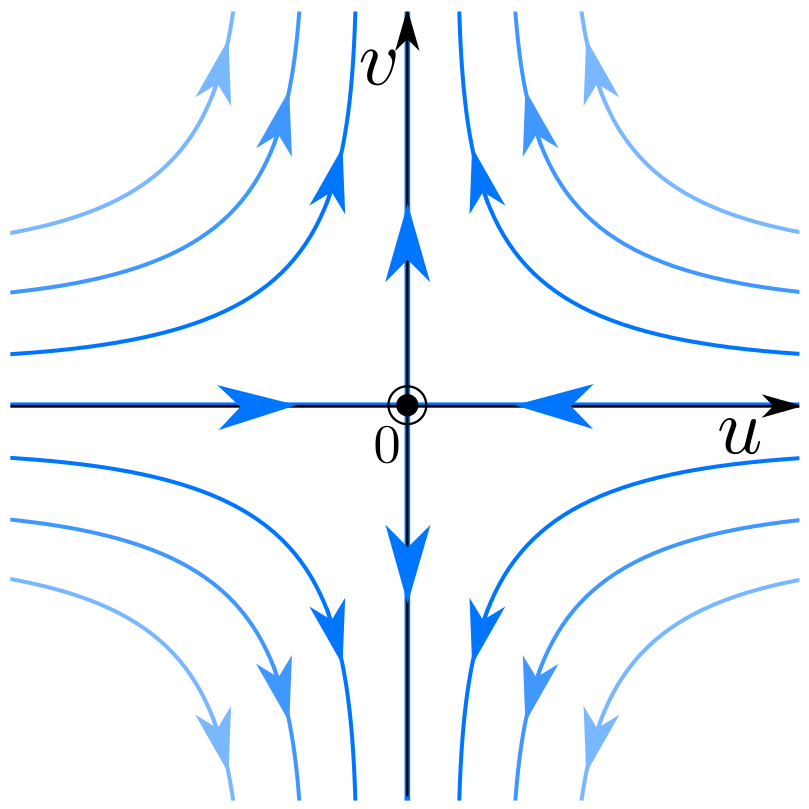
\includegraphics[scale=0.3]{assets/lectures_recent-53a0acd8.png} \end{gathered}
$$


Якщо $ \lambda_1 < 0,
  \lambda_2 > 0
$, то $
 \begin{gathered}
 u(t) \xrightarrow[t \to \infty]{} 0\\
 v(t) \xrightarrow[t \to \infty]{} \infty
 \end{gathered}$.
 Якщо $ \lambda_1 < 0,
  \lambda_2 > 0$, то  $
   \begin{gathered}
   u(t) \xrightarrow[t \to \infty]{} \infty\\
   v(t) \xrightarrow[t \to \infty]{} 0
   \end{gathered}.$\\
У другому випадку напрям руху траекторій відбуватиметься в інший бік.\\
Отже, перейшовши до початкових змінних, отримаємо, що за умови $\lambda_1 \cdot \lambda_2 < 0$ фазовий портрет має вигляд:

\begin{center} 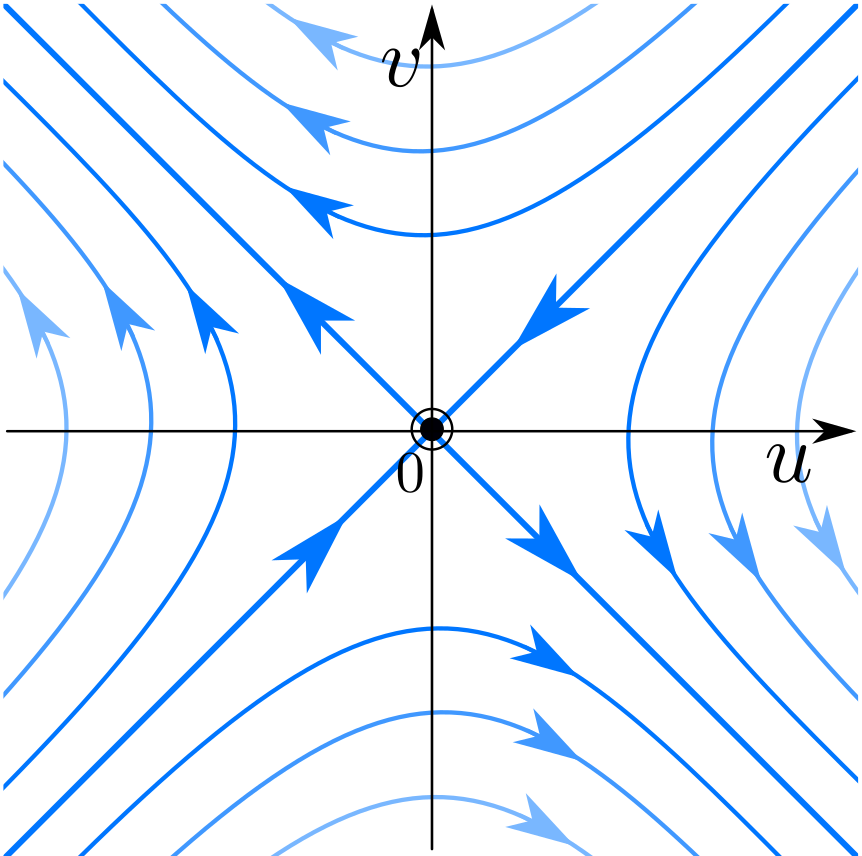
\includegraphics[scale=0.3]{assets/lectures_recent-0ebe704d.png} \end{center}

\begin{remark}
    Стрілки до нуля вздовж прямої, на якій лежить власний вектор, що відповідає $ \lambda_1 < 0$.\\
    Стрілки від нуля вздовж прямої, на якій лежить власний вектор, що відповідає $ \lambda_2 > 0$.
\end{remark}
Такий фазовий портрет називається \textbf{сідло}. Це завжди нестійке положення рівноваги.

\begin{example}
    $$
    \begin{cases}
        \dot{x} = x + 3y\\
        \dot{y} = 2x
    \end{cases} \qquad A = \begin{bmatrix}
     1 & 3 \\
     2 & 0
    \end{bmatrix}
    $$
    $$
    \det (A - \lambda I) = \begin{vmatrix}
      1-\lambda & 3 \\
      2 & - \lambda
    \end{vmatrix} = (1- \lambda)(-\lambda) - 6 = \lambda^2 - \lambda - 6 = 0
    $$
    $$
    \lambda_1 = 3 \quad \lambda_2 = -2 \Longrightarrow \text{сідло (нестійке)}
    $$
    Знаходимо власні вектори: \\
    $\lambda_1 = 3$
    $$
    \begin{bmatrix}
     -2 & 3\\
     2 & -3
    \end{bmatrix} \begin{bmatrix}
     h_1\\
     h_2
    \end{bmatrix} = \begin{bmatrix}
      0\\
      0
    \end{bmatrix} \qquad 2h_1 = 3 h_2 \Rightarrow \overrightarrow{h} = \begin{bmatrix}
     3 \\
     2
    \end{bmatrix}
    $$

    $\lambda_2 = -2$

    $$
    \begin{bmatrix}
     3 &3 \\
     2 & 2
    \end{bmatrix} \begin{bmatrix}
     g_1 \\
     g_2
    \end{bmatrix} = \begin{bmatrix}
     0 \\
     0
    \end{bmatrix} \qquad 2 g_1 =-2 g_2 \Rightarrow \overrightarrow{g} = \begin{bmatrix}
     1 \\
     -1
    \end{bmatrix}
    $$
    Отримали такий фазовий портрет:
    \begin{center} 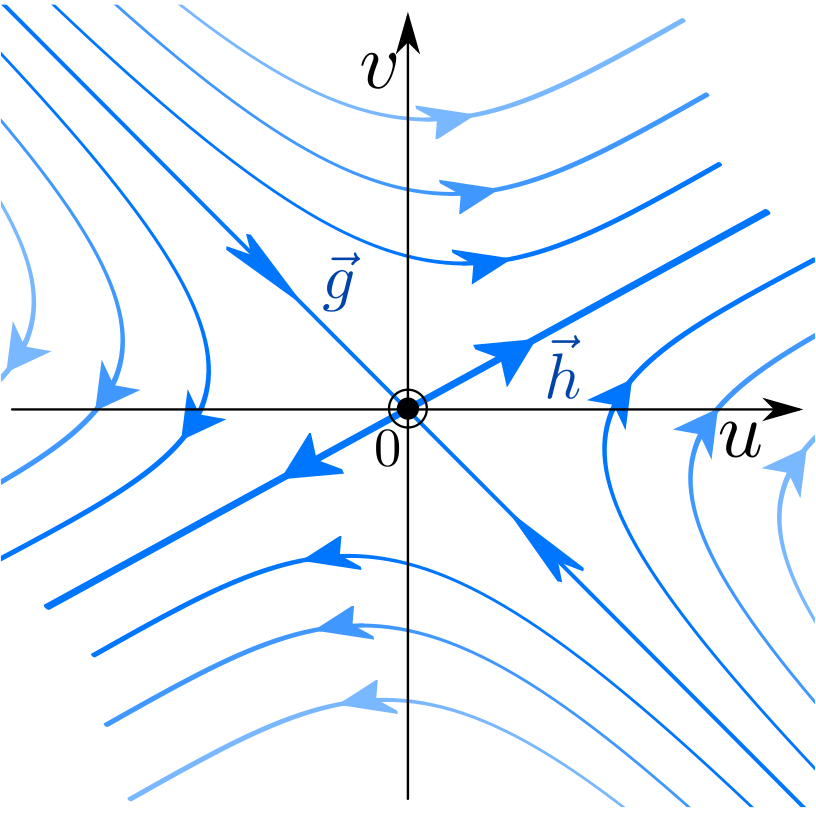
\includegraphics[scale=0.3]{assets/lectures_recent-c4b9c37b.png} \end{center}
\end{example}


3. Нехай $ \lambda_1 = \lambda_2 = \lambda \in \mathbb{R}$.\\
a) Матриця $A$ - діагональна.
$$
  A = \begin{bmatrix}
     \lambda & 0 \\
     0 & \lambda
    \end{bmatrix} \Longrightarrow \begin{cases}
        \dot{x} = \lambda x\\
        \dot{y} = \lambda y
    \end{cases}
$$
В такому випадку, фазовий портрет називають \textbf{диктричний вузол.}

\begin{center} 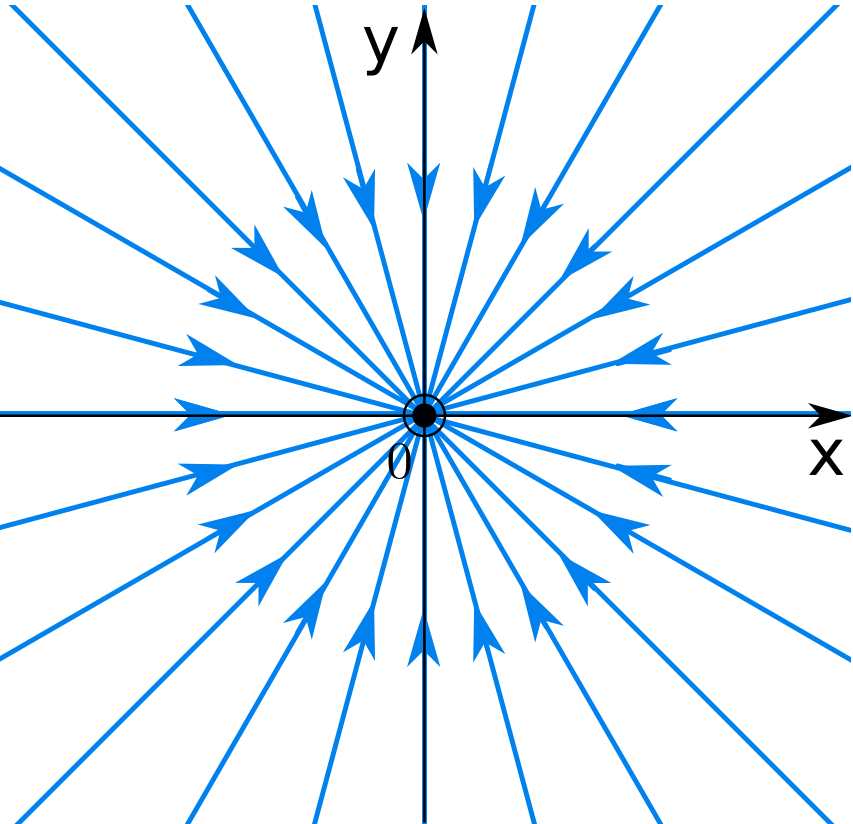
\includegraphics[scale=0.3]{assets/lectures_recent-ab36e3f3.png} \end{center}


Якщо $ \lambda < 0 $ - ас. стійкий (стрілки до нуля).\\
Якщо $ \lambda > 0 $ - нейстійкий (стрілки від нуля). \\
б) Матриця $A$ - недіагональна. В такому разі, фазовий портрет називають \textbf{вироджений вузол.}\\
- якщо $ \lambda < 0 $ - ас. стійкий ( стрілки до нуля ).\\
- якщо $ \lambda > 0 $ - нестійкий (стрілки від нуля).\\
Вироджений вузол може бути двох видів:
\begin{center} 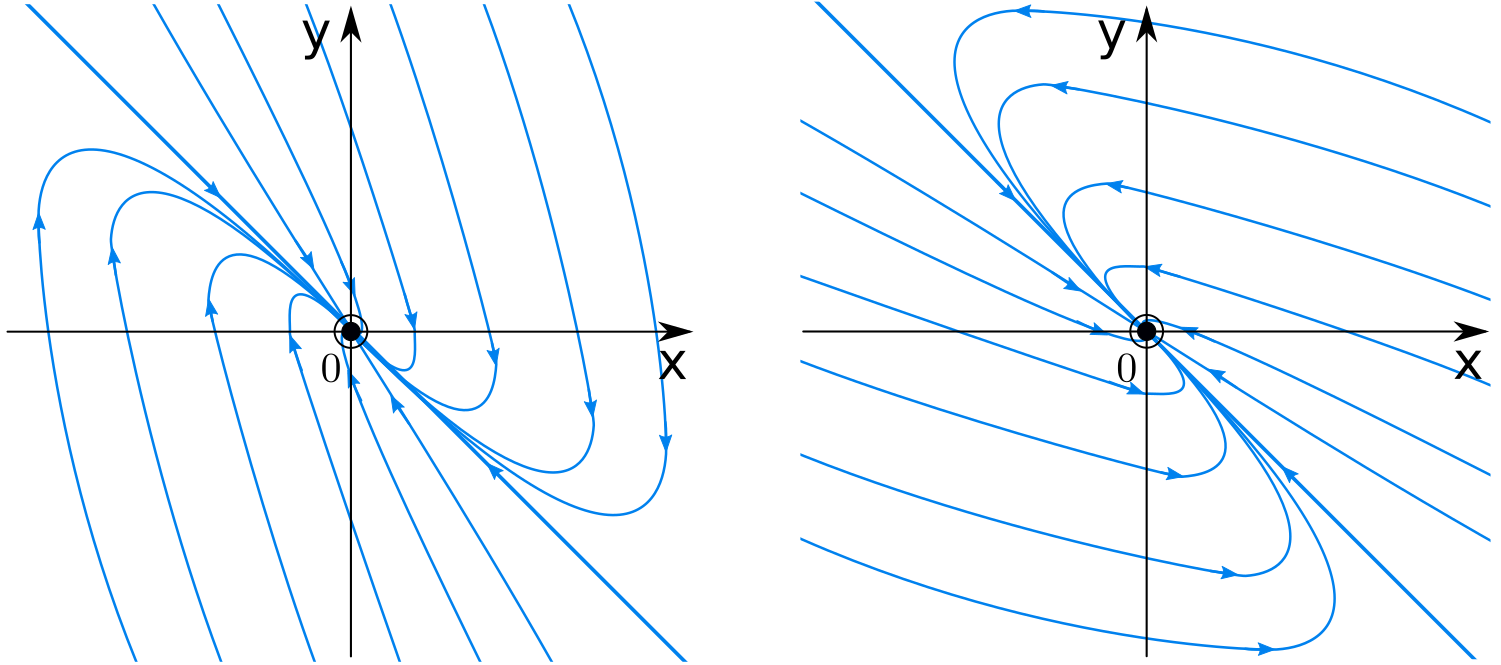
\includegraphics[scale=0.25]{assets/lectures_recent-b526bf37.png} \end{center}

Для визначення типу виродженого вузла потрібно визнгачити напрям вектора фазової швидкості $ \begin{bmatrix}
 \overrightarrow{x} \\
 \overrightarrow{y}
\end{bmatrix}$ в довільній точці, що не дорівнює нулю системи координат. Цей напрям має співпадати із напрямами руху по фазовій траєкторії (до нуля або від нуля).

\begin{example}
    $$
    \begin{cases}
        \overrightarrow{x} = 2y - 3x\\
        \overrightarrow{y} = y - 2x
    \end{cases} \qquad A = \begin{bmatrix}
     -3 & 2 \\
     -2 & 1
    \end{bmatrix}
    $$

    $$
    \det{ \left( A - \lambda I  \right) } = \begin{vmatrix}
      -3 - \lambda & 2 \\
      -2 & 1 - \lambda
    \end{vmatrix} = ( -3 - \lambda ) ( 1 -\lambda) + 4 =  \lambda^2 + 2 \lambda + 1 =
    $$
    $$
    = ( \lambda+ 1) ^2 = 0 \Longrightarrow  \lambda = -1 - \text{кратності 2. }
    $$
З попереднього випливає, що фазовим портретом буде асимптотично стійкий вироджений вузол (стрілки до нуля).
Знайдемо власний вектор:
$$
\begin{bmatrix}
 -2 & 2 \\
 -2 & 2
\end{bmatrix} \begin{bmatrix}
 h_1 \\
 h_2
\end{bmatrix} = \begin{bmatrix}
 0 \\
 0
\end{bmatrix} \qquad h_1 = h_2 \Rightarrow \overrightarrow{h} = \begin{bmatrix}
 1 \\
 1
\end{bmatrix}
$$

\begin{center} 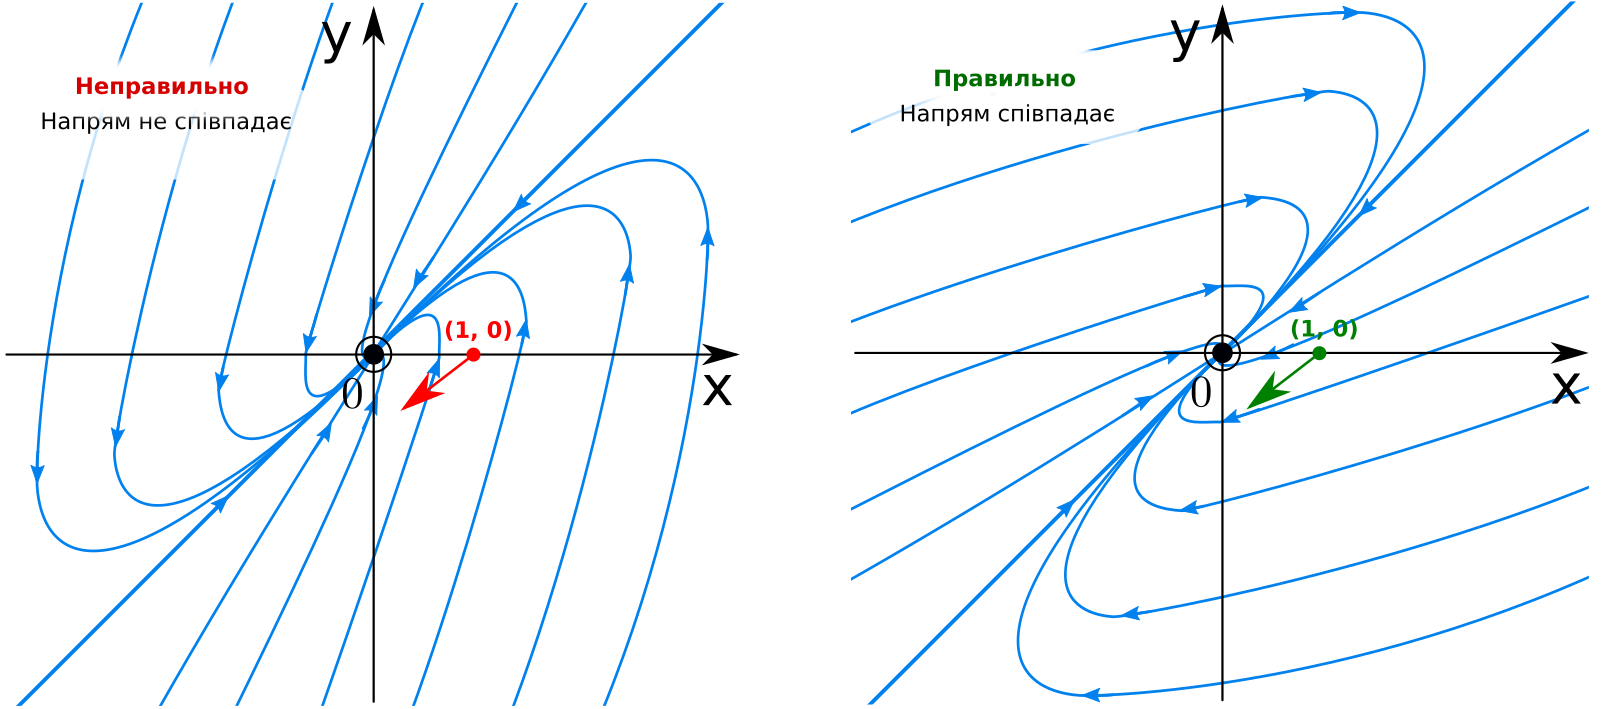
\includegraphics[scale=0.3]{assets/lectures_recent-f0de3cfc.png} \end{center}

Візьмемо т. (1, 0):
$$
\begin{bmatrix}
 \dot{x} \\
 \dot{y}
\end{bmatrix} \Bigg|_{(1,0)} = \begin{bmatrix}
 -3 \\
 -2
\end{bmatrix} \Longrightarrow \begin{gathered}
 x_k = -3 \\
 y_k = -2
\end{gathered}
$$

\end{example}

4. $\lambda_{1, 2} - \alpha \pm i\beta, \alpha\neq 0$. В такому випадку, фазовий портрет називається \textbf{фокус}. Якщо $ \alpha > 0$ - нестійкий. Якщо $ \alpha < 0$ -- ас. стійкий.
Фазовий портрет ''фокус'' може бути двох видів:
\begin{center} 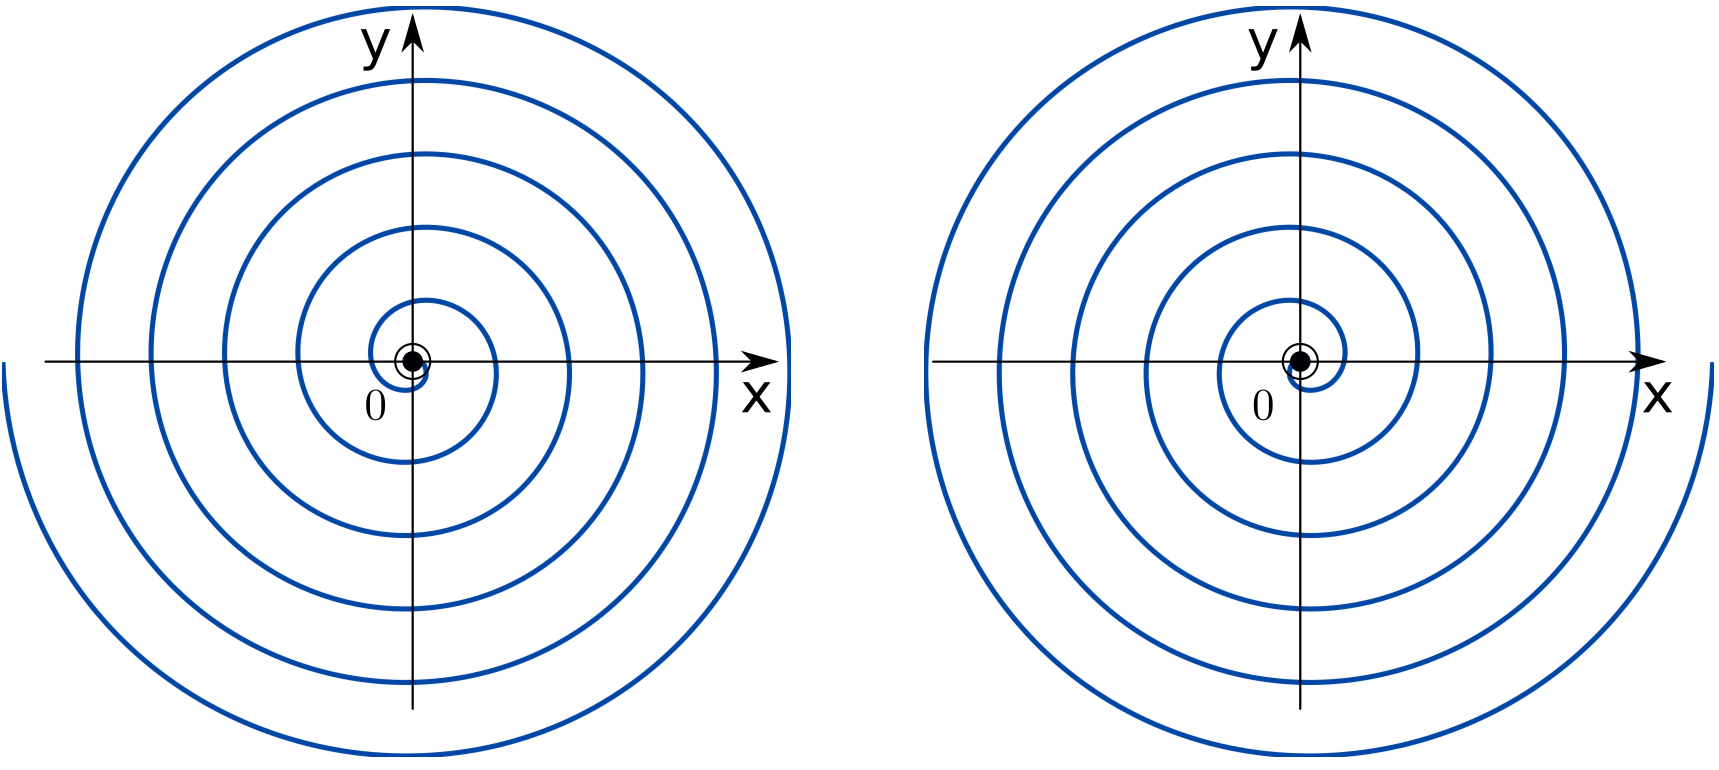
\includegraphics[scale=0.3]{assets/lectures_recent-9fe11a21.png} \end{center}
Для визначення типу фокуса визначаємо напрям вектора фазової швидкості в довільній точці, що не дорівнює нулю.

\begin{example}
    $$
    \begin{cases}
        \dot{x } = x - 2y\\
        \dot{y} = 4x - 3y
    \end{cases} \qquad A = \begin{bmatrix}
     1 & -2 \\
     4 & -3
    \end{bmatrix}
    $$
    $$ \det{(A - \lambda I)} = \begin{vmatrix}
      1- \lambda & -2 \\
      4 & -3-\lambda
    \end{vmatrix}  = ( 1- \lambda) (-3 - \lambda) + 8 = \lambda^2 + 2 \lambda + 5 = 0$$
$$
D = -16 \quad \lambda_{1,2} = \frac{-2 \pm 4i}{2} = -1 \pm 2i
$$
Асимптотично стійкий фокус (стрілки до нуля).
\begin{center} 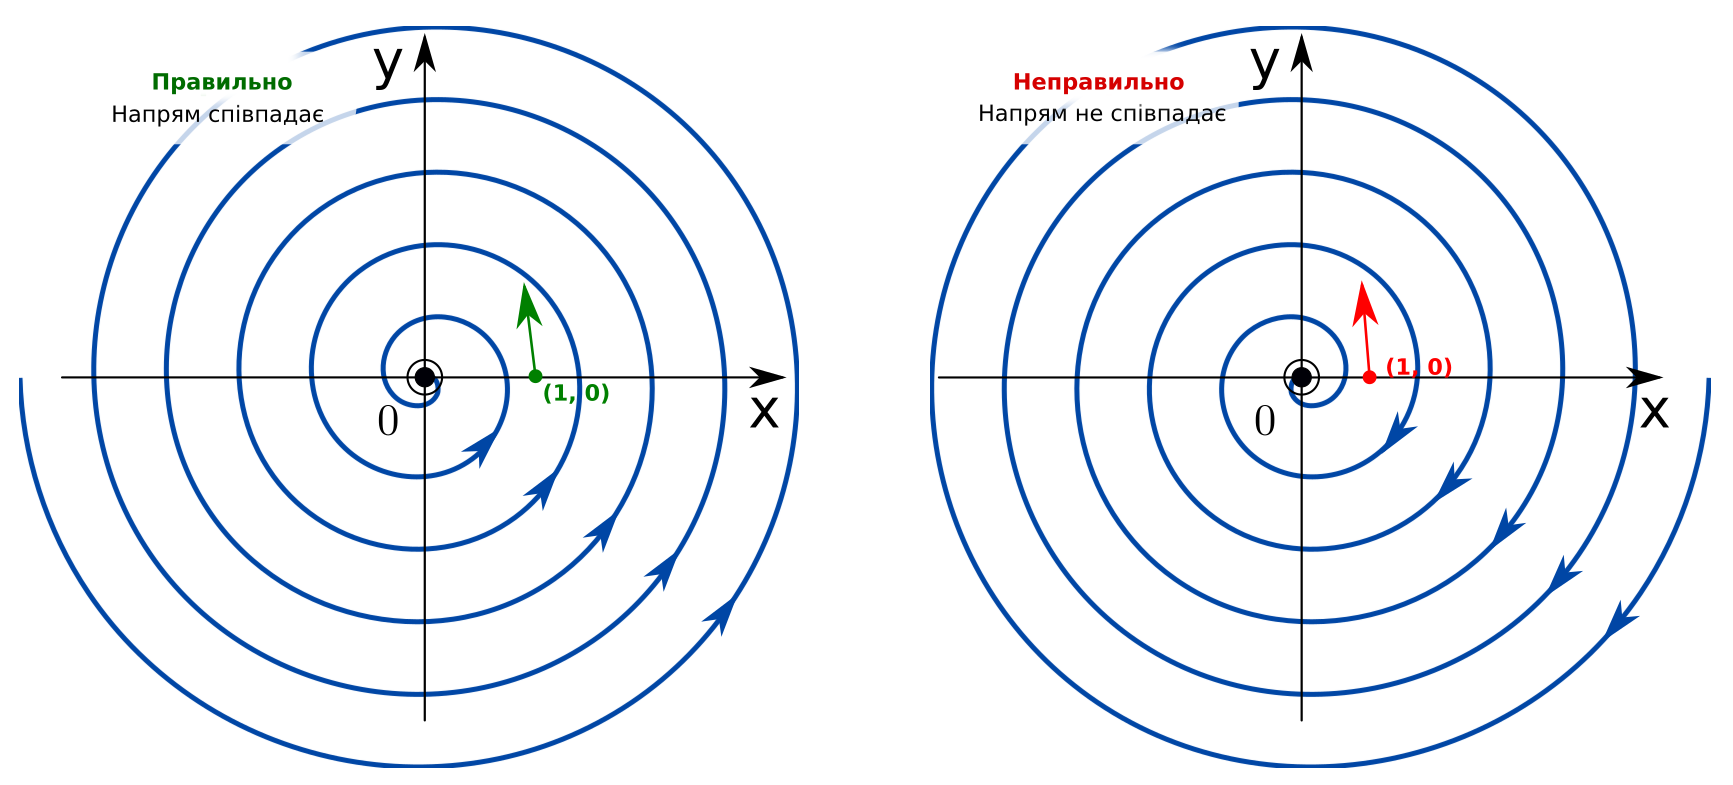
\includegraphics[scale=0.27]{assets/lectures_recent-b90426e3.png} \end{center}
Візьмемо точку (1, 0) для перевірки:

$$
\begin{bmatrix}
 \dot{x}\\
 \dot{y}
\end{bmatrix}\Bigg|_{(1,0)} - \begin{bmatrix}
 1 \\
 4
\end{bmatrix} \qquad \begin{gathered}
 x_k -1 = 1 \\
 y_k - 0 = 4
\end{gathered} \Rightarrow \begin{gathered}
 x_k = 2 \\
 y_k  = 4
\end{gathered}
$$
Отримали: $(1,0) \to (2, 4)$. Перевіримо за виглядом фазового портрета вище.
\end{example}

5.$ \lambda_{1,2} = \pm i \beta$. За таких власних чисел, фазовий портрет називається \textbf{центр.} (стійкий, але не асимптотично стійкий)
\begin{center} 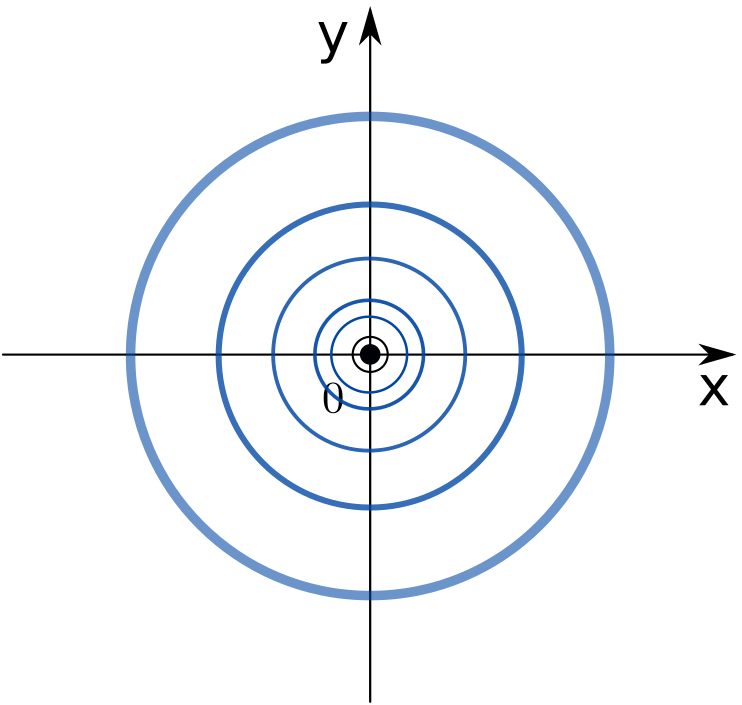
\includegraphics[scale=0.3]{assets/lectures_recent-2982f611.png} \end{center}

\begin{example}
    $$
    \begin{cases}
        \dot{x} = -2 x - 5y \\
        \dot{y} = 2x + 2y
    \end{cases} \qquad A = \begin{bmatrix}
     -2 & -5\\
     2 & 2
    \end{bmatrix}
    $$
    $$
    \det{(A - \lambda I)} = \begin{vmatrix}
      -2-\lambda & -5 \\
      2 & 2 -\lambda
    \end{vmatrix}  = \lambda^2 + 6 = 0 \Rightarrow \lambda = \pm i \sqrt{6} \Rightarrow \text{центр}
    $$
    Візьмемо т. (1, 0):
    $$
\begin{gathered}
\begin{bmatrix}
 \dot{x}\\
 \dot{y}
\end{bmatrix}\Bigg|_{(1,0)} = \begin{bmatrix}
 -2 \\
 2
\end{bmatrix} \\ \begin{cases}
  x_k -1 = -2\\
  y_k  - 0 = 2
\end{cases} \\
\begin{cases}
x_k = -1\\
    y_k  =2
\end{cases}
\end{gathered}\qquad    \begin{gathered} 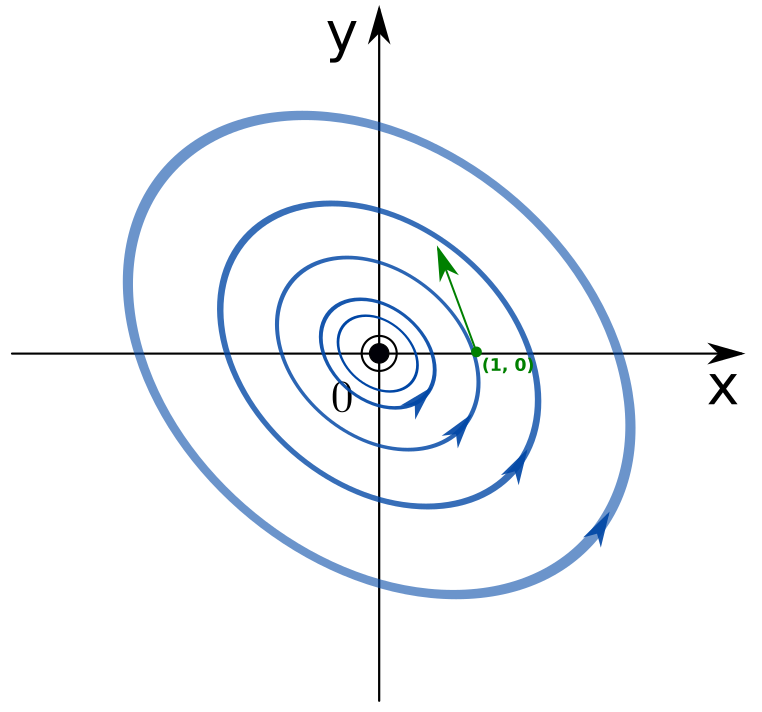
\includegraphics[scale=0.3]{assets/lectures_recent-1467e19e.png} \end{gathered}
    $$


\end{example}
6. Нехай $ \det A = 0$ (вирджений випадок).\\
$$
\det A  =  \begin{vmatrix}
  a & b\\
  c & d
\end{vmatrix} = ad - bc  = 0 \Rightarrow \frac{a}{c} = \frac{b}{d} = 0 \quad \begin{gathered}
 a = kc\\
 b = kd
\end{gathered}
$$
$$
\begin{cases}
    \dot{x} = ax+ by\\
    \dot{y} = k(ax + by)
\end{cases} \Rightarrow ax + by  = 0 \text{ - пряма положень рівноваги.}
$$

$$
\det ( A - \lambda I) = \begin{vmatrix}
  a - \lambda & b\\
  ka & kb - \lambda
\end{vmatrix} = (a-\lambda)*(kb- \lambda) - kab =
$$
$$
 = akb - a \lambda - kb \lambda +  \lambda^2 - kab = \lambda^2 - (a + kb) \lambda =0
 $$
 $$
 \lambda = 0 \qquad \lambda = a + bk
 $$

 a) Прямі паралельні власному вектору, що відповідає власному числу $\lambda =  a + bk$\\
 $\lambda > 0 $ - стрілки від нуля.\\
 $\lambda < 0 $ - стрілки до нуля.\\

 \begin{center} 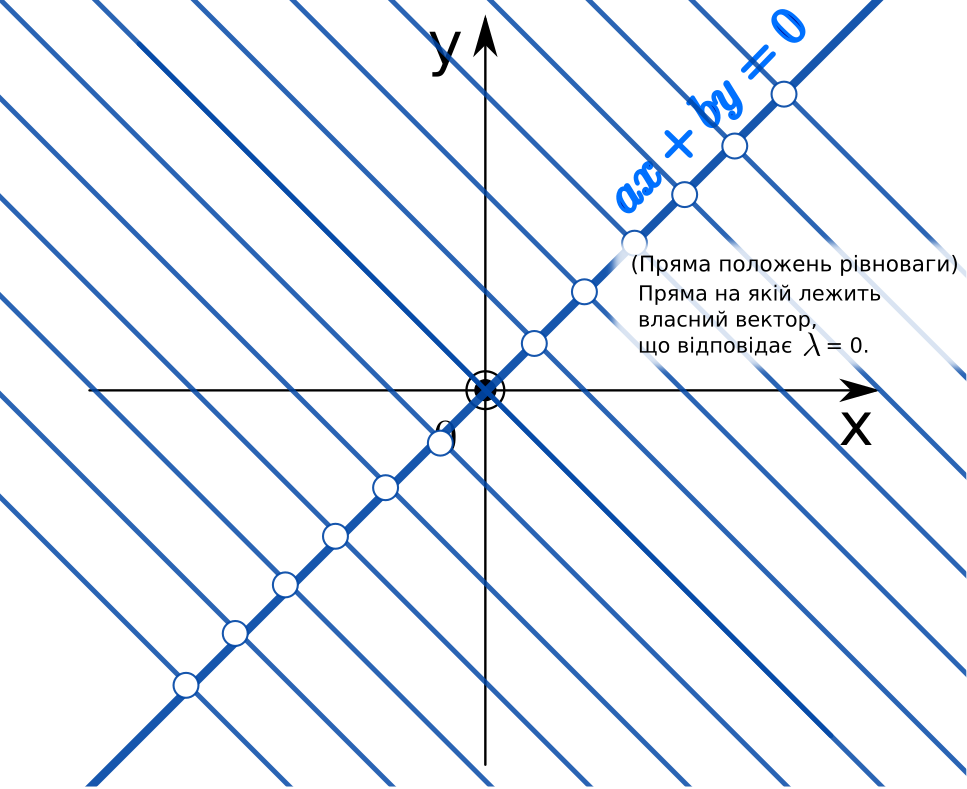
\includegraphics[scale=0.257]{assets/lectures_recent-058ceaff.png} \end{center}
b) $ \lambda_1 =  \lambda_2 = 0 \quad (a = - bk)$

\begin{center} 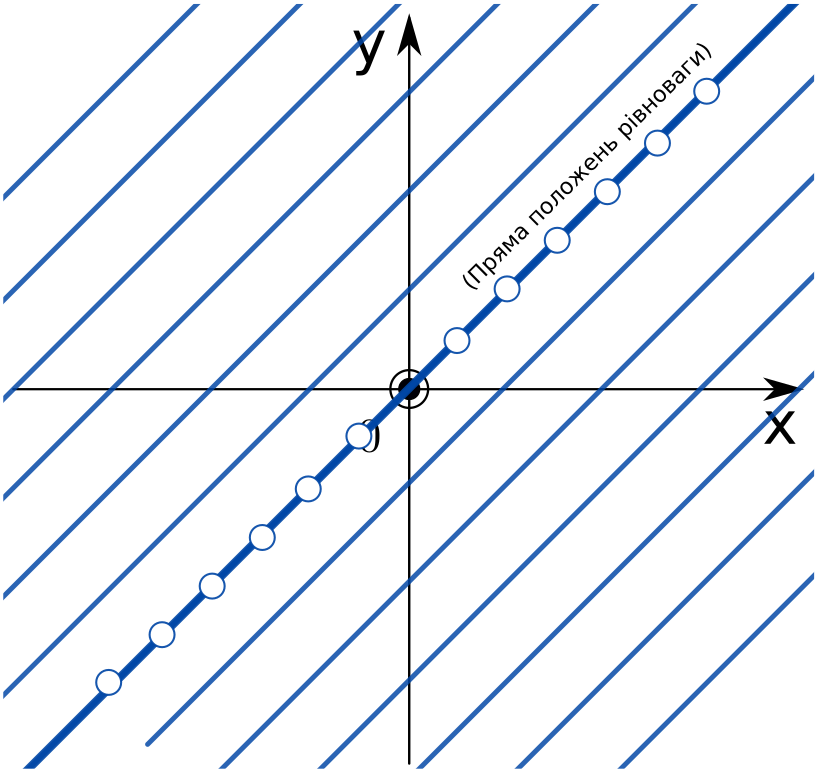
\includegraphics[scale=0.3]{assets/lectures_recent-49093f01.png} \end{center}

\section{Лекція 3}
\subsection{Стійкість за першим наближенням}

Розглянемо систему:
\begin{equation}\label{1sdp}
  \dot{\vect{x}} = \overrightarrow{f}(\overrightarrow{x}(t)), \quad \overrightarrow{f}: D \rightarrow \mathbb{R}^n, \quad D \subset \mathbb{R}^n
\end{equation}
Функція $f$ один раз неперервно диференційована ($f \in C^1(D)$), це гарантує існування та єдиність довільної задачі Коші: $\quad \forall t_0 \in \mathbb{R} \quad \forall x_0 \in D$. \\
Система \eqref{1sdp} -- автономна система n-ого порядку, $\overrightarrow{f}$ не залежить явно від $t$.
Нехай $\overrightarrow{f}(\overrightarrow{0}) = \overrightarrow{0}$, тобто $\overrightarrow{x} = \overrightarrow{0}$ -- положення рівноваги системи \eqref{1sdp}, якщо це не так і $\overrightarrow{x} = \overrightarrow{x}^*$ -- положення рівноваги, то заміна $\overrightarrow{z} = \overrightarrow{x} - \overrightarrow{x}^*$ зведе задачу до положення рівноваги $\overrightarrow{z} = \overrightarrow{0}$.

\textbf{Завдання: } дослідити на стійкість розв'язок $\overrightarrow{x} = \overrightarrow{0}$ системи \eqref{1sdp}. Оскільки $\overrightarrow{f} \in C^1(D)$, то в деякому околі $B_r(\overrightarrow{0})$ функцію $\overrightarrow{f}$ можно подати у вигляді:
\begin{equation*}
  \overrightarrow{f}(\overrightarrow{x}) = \dfrac{\partial \overrightarrow{f}}{\partial \overrightarrow{x}}(\overrightarrow{0}) \cdot \overrightarrow{x} + f_1(\overrightarrow{x}), \text{ де } f_1(\overrightarrow{x}) = o(||\overrightarrow{x}||), \quad \overrightarrow{x} \rightarrow \overrightarrow{0} \quad \text{ (формула Тейлора)}
\end{equation*}
Позначимо: $\dfrac{\partial \overrightarrow{f}}{\partial \overrightarrow{x}}(\overrightarrow{0}) = A$ -- стала $n \times n$ матриця Якобі. Тоді в околі точки $\overrightarrow{0}$ система \eqref{1sdp} набуває вигляду:
\begin{center}
  \fbox{$\overrightarrow{x}'(t) = A\overrightarrow{x}(t) + o(||\overrightarrow{x}||)$}
\end{center}
\bd ЛОС:
\begin{equation*}
  \overrightarrow{x}' = A\overrightarrow{x}, \text{ де } \quad A = \dfrac{\partial\overrightarrow{f}}{\partial\overrightarrow{x}}(\overrightarrow{0})
\end{equation*}
називається с-мою 1-ого наближення (або лінеаризованою с-мою) для \eqref{1sdp}.
\ed
\begin{boxteo}[про стійкість за першим наближенням]
  Розглянемо два випадки:
  \begin{enumerate}
    \item Якщо $\forall \lambda$ -- власні матриці $A$ справедливо, що $\Re \lambda < 0$, то розв'язок $\overrightarrow{x} = \overrightarrow{0}$ системи \eqref{1sdp} асимптотично стійкий.
    \item Якщо існує таке власне число матриці $А$, що $\Re \lambda > 0$, то розв'язок $\overrightarrow{x} = \overrightarrow{0}$ системи \eqref{1sdp} нестійкий.
  \end{enumerate}
\end{boxteo}

\textbf{Приклад 1.}
\begin{gather*}
  \begin{cases}
     \dot{x} = -\ln(1+y) + 2x + \sin x \quad  (=f_1(x, y))\\
     \dot{y} = e^x + \sin(x+y) - \cos^2y \quad (=f_2(x, y))
  \end{cases}
\end{gather*}
Завдання: дослідити на стійкість розв'язок: $\begin{bmatrix} x \\ y \end{bmatrix} = \begin{bmatrix} 0 \\ 0 \end{bmatrix}$ системи.
\begin{spacing}{2.5}
\begin{gather*}
  A = \left. \begin{bmatrix}
    \dfrac{\partial f_1}{\partial x}   &   \dfrac{\partial f_1}{\partial y} \\
    \dfrac{\partial f_2}{\partial x}   &   \dfrac{\partial f_2}{\partial y}
  \end{bmatrix} \right|_{(0,0)} =
  \left. \begin{bmatrix}
   2 + \cos x &  -\dfrac{1}{1+y} \\
   e^x + \cos(x+y)  &  \cos(x+y) + 2\cos{y}\sin{y}
 \end{bmatrix} \right|_{(0,0)}
\end{gather*}
\end{spacing}
Отримуємо, що $A = \begin{bmatrix} 3 & -1 \\ 2 & 1\end{bmatrix}$, тоді $\det(A - \lambda I) =  \begin{vmatrix} 3 - \lambda & -1 \\ 2 & 1 - \lambda \end{vmatrix}$. \\
Маємо: $(3 - \lambda)(1 - \lambda) + 2 = \lambda^2 - 4\lambda + 5 = 0, D = 16 - 4 \cdot 5 = -4 < 0$, звідси $\lambda_{1, 2} = 2 \pm i$, $\Re \lambda > 0$, тоді розв'язок $(x, y)^T = (0, 0)^T $ нестійкий.

\textbf{Приклад 2.}
\begin{gather*}
  \begin{cases}
     \dot{x} = \tan(x+y) - y \quad  (=f_1(x, y))\\
     \dot{y} = 3\sin{x} + 2e^y - 2 \quad (=f_2(x, y))
  \end{cases}
\end{gather*}

\begin{spacing}{2.5}
\begin{gather*}
  A = \left. \begin{bmatrix}
    \dfrac{\partial f_1}{\partial x}   &   \dfrac{\partial f_1}{\partial y} \\
    \dfrac{\partial f_2}{\partial x}   &   \dfrac{\partial f_2}{\partial y}
  \end{bmatrix} \right|_{(0,0)}  =
  \left.\begin{bmatrix}
     \dfrac{1}{\cos^2(x+y)} & \dfrac{1}{\cos^2(x+y) - 1} \\
    3 \cos x & 2e^y
  \end{bmatrix} \right|_{(0,0)}  =
  \begin{bmatrix}
    1 & 0 \\
    3 & 2
  \end{bmatrix}
\end{gather*}
\end{spacing}

Тоді $\det(A - \lambda I) =  \begin{vmatrix} 1 - \lambda & 0 \\ 3 & 2 - \lambda \end{vmatrix} = (1 - \lambda)(2 - \lambda) = 0. \\ $ Отримуємо: $\lambda_1 = 1,  \lambda_2 = 2,  \Re \lambda > 0$, тоді розв'язок $(x, y)^T = (0, 0)^T $ нестійкий.

\textbf{Зауваження. } Випадок, коли $\forall \lambda : \Re \lambda \leq 0$ та $\exists \lambda : \Re \lambda = 0$ є критичним. \\ В цьому випадку за системою першого наближення нічого сказати не можна.

\textbf{Доведення теореми 3.1. } Пункт 1. Нехай для будь-якого власного числа матриці $A$ справедливо, що $\Re < 0$. Доведемо, що розв'язок $\overrightarrow{x} = \overrightarrow{0}$ асимптотично стійкий. За означенням: $\forall \varepsilon > 0 \quad \forall t_0 \quad \exists \delta > 0 : \forall$ розв'язку $\overrightarrow{x}(t)$ з початковими умовами $\overrightarrow{x}(t_0) = \overrightarrow{x}_0$ такого, що $||\overrightarrow{x}_0|| < \delta$ справедливо, що:
\begin{enumerate}
  \item $||\overrightarrow{x}(t)|| < \varepsilon$ (стійкість).
  \item $||\overrightarrow{x}(t)|| \xrightarrow[t \to \infty]{} 0$ (асимптотична стійкість).
\end{enumerate}

Таким чином, щоб довести твердження потрібно оцінити норму $||x(t)||$. Подальше доведення теореми потребує двох лем.

\begin{boxlema}[Гронуолла-Беллмана]
Нехай $a(t), u(t) \in C([t_0, t_1]), a(t) \geq 0 \\ \forall t \in [t_0, t_1]$ і числа $c \geq 0$ та $b \geq 0$ такі, що: $$\forall t \in [t_0, t_1] \quad u(t) \leq c + b(t - t_0) + \int\limits_{t_0}^{t}a(s)u(s)\mathrm{d}s$$
Тоді $\forall t \in [t_0, t_1]:$ $$ u(t) \leq (c + b(t-t_0))\exp \left\lbrace {\int\limits_{t_0}^{t} a(s)\mathrm{d}s} \right\rbrace$$
\end{boxlema}

\begin{proof}
Розглянемо допоміжну функцію: $v(t) = c  +  b(t-t_0) + \mathop{\mathlarger{\int}}\limits_{t_0}^{t}a(s)u(s)\mathrm{d}s$ Тоді: $$ v(t_0) = c; \quad u(t) \leq v(t) \quad \forall t \in [t_0, t_1]; \quad v'(t) = b + a(t)u(t) \leq b + a(t)v(t)$$ Отже, $v'(t) \leq b + a(t)v(t)$, домножимо ліву і праву частину на $\exp \left\lbrace {-\int\limits_{t_0}^{t} a(s)\mathrm{d}s} \right\rbrace$: $$v'(t) \cdot
\exp \left\lbrace {-\int\limits_{t_0}^{t} a(s)\mathrm{d}s} \right\rbrace \leq b \cdot \exp \left\lbrace {-\int\limits_{t_0}^{t} a(s)\mathrm{d}s} \right\rbrace + a(t) \cdot \exp \left\lbrace {-\int\limits_{t_0}^{t} a(s)\mathrm{d}s} \right\rbrace \cdot v(t) $$
Перенесемо один з множників наліво: $$v'(t) \cdot \exp \left\lbrace {-\int\limits_{t_0}^{t} a(s)\mathrm{d}s} \right\rbrace - a(t) \cdot \exp \left\lbrace {-\int\limits_{t_0}^{t} a(s)\mathrm{d}s} \right\rbrace \cdot v(t)\leq b \cdot \exp \left\lbrace {-\int\limits_{t_0}^{t} a(s)\mathrm{d}s} \right\rbrace $$

Використаємо властивість похідної: $$\mathlarger{\Bigg(}v(t) \cdot \exp \left\lbrace {-\int\limits_{t_0}^{t} a(s)\mathrm{d}s} \right\rbrace \mathlarger{\Bigg)}' \leq b \cdot \exp \left\lbrace {-\int\limits_{t_0}^{t} a(s)\mathrm{d}s} \right\rbrace $$

Проінтегруємо ліву і праву частини від $t$ до $t_0$:
$$ v(t) \cdot \exp \left\lbrace {-\int\limits_{t_0}^{t} a(s)\mathrm{d}s} \right\rbrace - \underbrace{v(t_0)}_{const} \leq \int\limits_{t_0}^{t}b \cdot \underbrace{\exp \left\lbrace {-\int\limits_{t_0}^{t} a(s)\mathrm{d}s} \right\rbrace }_{1}\mathrm{d}t$$
Звідси отримуємо наступне: $$ v(t) \cdot \exp \left\lbrace {-\int\limits_{t_0}^{t} a(s)\mathrm{d}s} \right\rbrace  \leq c + b(t - t_0) $$
Остаточно: $$ u(t) \leq v(t) \leq (c + b(t - t_0)) \cdot \exp \left\lbrace {\int\limits_{t_0}^{t} a(s)\mathrm{d}s}  \right\rbrace $$
\end{proof}

\begin{boxlema}
  Нехай $\exists \gamma > 0 : \forall \lambda$ -- власного числа матриці $A: \Re \lambda < - \gamma$, тоді $$\exists K > 0 : ||e^{At}|| \quad \leq  \quad K \cdot e^{-\gamma t} \quad \forall t \geq 0$$
  Без доведення. $\quad \blacksquare$
\end{boxlema}

Повернемось до доведення теореми. \\ Візьмемо $\forall \varepsilon > 0$ та $\forall \delta : 0 < \delta < \varepsilon$ (поки що довільне $\delta$). Також візьмемо довільну початкову умову $\overrightarrow{x}(t_0) = \overrightarrow{x}_0$, де $||\overrightarrow{x}_0|| < \delta$ (зауважимо, що $||\overrightarrow{x}_0|| < \delta < \varepsilon$) і розглянемо $\overrightarrow{x}(t)$ -- розв'язоу системи з початковими умовами $\overrightarrow{x}(t_0) = \overrightarrow{x}_0$. За теоремою про продовження розв'язок $\overrightarrow{x}(t)$ можна продовжити до межі області: $B_{\varepsilon}(\overrightarrow{0}) = \left\{ \overrightarrow{x} \quad | \quad ||\overrightarrow{x}|| < \varepsilon \right\}$. Тоді можливими є два варіанти:
\begin{enumerate}
  \item $\exists t* > t_0 : ||\overrightarrow{x}(t)|| < \varepsilon \quad \forall t \in [t_0, t*)$ та $\overrightarrow{x}(t*) = \varepsilon$ (межа області досягнута).
  \item $\forall t \geq t_0 : ||\overrightarrow{x}|| < \varepsilon$ (межа області не досягається за скінченний час. Отже, розв'язок існує $\forall t \geq t_0$ та $||\overrightarrow{x}(t)|| < \varepsilon$, що автоматично означає стійкість).
\end{enumerate}

У першому випадку покладемо: $I = [t_0, t_1]$, а у другому: $I = [t_0, +\infty)$ та розглянемо на $I$ наступну задачу Коші: $$\begin{cases} u'(t) = A\overrightarrow{u}(t) + \overrightarrow{f}_1(\overrightarrow{x}(t)) \\ \overrightarrow{u}(t_0) = \overrightarrow{x}_0 \end{cases}$$ Це ЛНС, задача Коші має единий розв'язок. Підставивши $\overrightarrow{x}(t) = \overrightarrow{u}(t)$, переконуємось, що $\overrightarrow{u}(t) = \overrightarrow{x}(t)$ -- єдиний розв'язок задачі Коші. Можемо знайти його методом варіації довільної сталої. Загальний розв'язок ЛНС = загальний розв'язок ЛОС + частинний розв'язок ЛНС. Частинний розв'язок ЛНС будемо шукати у вигляді $e^{At} \cdot \overrightarrow{C}(t)$.

$$e^{At} \cdot \overrightarrow{C}'(t) + Ae^{At} \cdot \overrightarrow{C}(t) = Ae^{At} \cdot \overrightarrow{C}(t) + \overrightarrow{f}_1(\overrightarrow{x}(t))$$

Звідси отримуємо: $$\overrightarrow{C}'(t) \!=\! e^{-At} \overrightarrow{f}_1(\overrightarrow{x}(t)) \Longrightarrow \overrightarrow{u}_r(t) \!=\!
e^{At}  \int\limits_{t_0}^{t} e^{-As} \overrightarrow{f}_1(\overrightarrow{x}(s))\mathrm{d}s \!=\!\!\! \int\limits_{t_0}^{t} e^{A(t-s)}\overrightarrow{f}_1(\overrightarrow{x}(s))\mathrm{d}s
$$

Загальний розв'язок ЛНС: $\overrightarrow{u}(t) = e^{At}  \overrightarrow{C} + \mathop{\mathlarger{\int}}\limits_{t_0}^{t} e^{A(t - s)} \overrightarrow{f}_1(\overrightarrow{x}(s))\mathrm{d}s$, звідси знаходимо розв'язок даної задачі Коші $\quad \overrightarrow{u}(t_0) = \overrightarrow{x}_0 : \overrightarrow{x}_0 = e^{At_0} \cdot \overrightarrow{C} \quad \Longrightarrow \quad \overrightarrow{C} = e^{-At_0} \cdot \overrightarrow{x}_0$

Отже, $$\overrightarrow{u}(t) = \overrightarrow{x}(t) = e^{A(t - t_0)}\overrightarrow{x}_0 + \mathop{\mathlarger{\int}}\limits_{t_0}^{t} e^{A(t - s)} \overrightarrow{f}_1(\overrightarrow{x}(s))\mathrm{d}s$$
Таким чином, знайшли розв'язок $\overrightarrow{x}(t)$, який маємо оцінити.

Використаємо лему 2. Оскільки $\forall \lambda : \Re \lambda < 0$, то $\exists \gamma > 0 : \Re \lambda < -\gamma$. Тоді: $$\exists K > 0 : ||e^{At}|| \leq K \cdot e^{-\gamma t}$$
Маємо: $$ ||\overrightarrow{x}(t)|| \leq K \cdot e^{-\gamma(t - t_0)} \cdot || \overrightarrow{x}_0|| + \int\limits_{t_0}^{t} K \cdot e^{-\gamma(t - s)} ||\overrightarrow{f}_1(\overrightarrow{x}(s))||\mathrm{d}s$$
Звідси отримуємо: $$||\overrightarrow{x}(t)|| \cdot e^{\gamma(t - t_0)} \leq K||\overrightarrow{x}_0|| + K \int\limits_{t_0}^{t} e^{\gamma(s - t_0)} ||\overrightarrow{f}_1(\overrightarrow{x}(s))||\mathrm{d}s$$
Оцінимо $||\overrightarrow{f_1}(\overrightarrow{x}(s))||$. Зауважимо, що $\overrightarrow{f}_1(\overrightarrow{x}(s)) = \overrightarrow{\overrightarrow{0}}(||\overrightarrow{x}||)$ при $||\overrightarrow{x}|| \longrightarrow 0$. Отже,
$\forall \delta_1 > 0 \quad \exists \delta_2 > 0 : \forall x : ||\overrightarrow{x}|| < \delta_2 \text{ справедливо, що } ||\overrightarrow{f}_1(\overrightarrow{x})|| < \delta_1 ||\overrightarrow{x}||$. З попередніх міркувань: $$||\overrightarrow{x}(t)|| \cdot e^{\gamma(t - t_0)} \leq K \cdot \delta + K \cdot \delta_1 \int\limits_{t_0}^{t} e^{\gamma(s - t_0)} \cdot ||\overrightarrow{x}(s)||\mathrm{d}s$$
Застосуємо лему Гронуолла-Беллмана:

$$ u(t) = ||\overrightarrow{x}(t)|| \cdot e^{\gamma(t - t_0)}, \quad c = K \cdot \delta, \quad b = 0, \quad a = K \cdot \delta_1$$

Отримуємо: $$||\overrightarrow{x}(t)|| e^{\gamma(t - t_0)} \!\leq\! K \delta \exp \left\lbrace {\int\limits_{t_0}^{t} K \delta_1 \mathrm{d}s} \right\rbrace \!=\! K \delta e^{K \cdot \delta (t - t_0)} \!\Rightarrow\! ||\overrightarrow{x}(t)|| \!\leq\! K \delta e^{(-\gamma + K \cdot \delta_1)(t - t_0)}$$ Оберемо $\delta_1$ так, щоб $-\gamma + K \cdot \delta_1 < 0 \quad \Longrightarrow \quad \delta_1 < \dfrac{\gamma}{K}$, тоді $||\overrightarrow{x}(t)|| \leq K \cdot \delta < \varepsilon$ при $\delta < \dfrac{\varepsilon}{K}$ і, крім того, $||\overrightarrow{x}(t)|| \leq K \cdot \delta \cdot e^{(-\gamma + K \cdot \delta_1)(t - t_0)} \xrightarrow[t \to \infty]{} 0$, що означає стійкість та асимптотичну стійкість розв'язку $\overrightarrow{x} = \overrightarrow{0}$ за означенням (в означенні в якості $\delta$ можемо взяти найменше з $\delta, \quad \delta_1, \quad \delta_2$).\\ Випадок 2. поки ще залишається без доведення. $\blacksquare$ \\ \\
\textbf{Зауваження.} (про фазові портрети автономної системи другого порядку). Тип фазового портрету в околі положень рівноваги автономної системи другого порядку у випадку $\Re \lambda \neq 0$ визначається типом фазового портрету лінеаризованої системи (вузол, сідло, фокус, вироджений вузол залишається вузлом, сідлом, фокусом, виродженим вузлом відповідно). \\

\section{Лекція 4}
\subsection{Метод функцій Ляпунова}
Розглянемо систему:
\be \label{2spd}
 \overrightarrow{x}' = f(\overrightarrow{x})
\ee
дe $f: D \to \mathbb{R}^n, f\in C^{1} \left( D \right), D \subset \mathbb{R}^n $ та $\overrightarrow{f} ( \overrightarrow{0}) = 0$. \textbf{Задача. } Дослідити на стійкість розв'язок $ \overrightarrow{x} = \overrightarrow{0}$ системи \eqref{2spd}.
 \begin{defo}
  Функція $V : D \to \mathbb{R}, V \in C(D) $ називається додатньо(від'ємно)-визначеною в $D$, якщо:
\begin{enumerate}
  \item $V(0) = 0$.
  \item $V(x) > 0 \ (<0) \ \forall x \in D(\left\lbrace 0 \right\rbrace)$.
\end{enumerate}
 \end{defo}

 \begin{defo}
Похідною функції $ V : D \to \mathbb{R}$ в силу системи \eqref{2spd} називають функцію:
$$
\dot{V}_f(\overrightarrow{x}) =  \sum\limits_{i = 1}^{n}{ \frac{\partial V}{ \partial x_i} f_{i}( \overrightarrow{x}) } = <\nabla V \overrightarrow{x}, f(\overrightarrow{x})>
$$
 \end{defo}

\begin{defo}
  Нехай $B_{R} ( \overrightarrow{0} ) $ -- деякий окіл точки $ \overrightarrow{0} $. Функція $V \in C^{1} (B_{R} (\overrightarrow{0}))$ називається функцією Ляпунова системи \eqref{2spd}, якщо:
\begin{enumerate}
  \item $V$ -- додатно визначена.
  \item $\dot{V}_f (\overrightarrow{x}) \leq 0 \quad \forall x \in B_{R} ( \overrightarrow{0})$.
\end{enumerate}
\end{defo}

\begin{remark}
    Якщо $ V $ - від'ємно визначена і $ \dot{V}_f ( \overrightarrow{x}) \geq 0$, то: $$ - V ( \overrightarrow{x} ) - \text{ функція Ляпунова. }$$
\end{remark}

\begin{boxteo}[Ляпунова про стійкість]
  Якщо в деякій кулі $B_{R}( \overrightarrow{0}) $ існує функція Ляпунова для системи \eqref{2spd}, то розв'язок $ \overrightarrow{x} = \overrightarrow{0} $ системи \eqref{2spd} стійкий.
\end{boxteo}

\begin{proof}
   Нехай $ V \in C^{1} ( B_{R} ( \overrightarrow{0} ))$ -- функція Ляпунова. Доведемо, що розв'язок стійкий за означенням. Візьмемо $ \forall \varepsilon > 0, \varepsilon < \mathbb{R}$. Покладемо $ c( \varepsilon) \min\limits_{\overrightarrow{x} : ||\overrightarrow{x}|| = \varepsilon} V(\overrightarrow{x}) $. Тоді $ c(\varepsilon) > 0, $ бо $ V( \overrightarrow{x}) $ - додатно визначена. Виберемо $ \delta > 0 : 0 < \delta < \varepsilon $ таким чином, щоб: $ \forall \overrightarrow{x}: ||\overrightarrow{x}|| < \delta $ справдовується: $V (\overrightarrow{x}) < C(\varepsilon) $ ( таке $\delta$ існує в силу неперервності $V( \overrightarrow{x})$ та $V ( \overrightarrow{x}) =0 $). Візьмемо $\forall \overrightarrow{x}_0: ||\overrightarrow{x}_0||< \delta $ і розглянемо розв'язок $\overrightarrow{x} (t) $ з початковими умовами $ \overrightarrow{x}(t_0) = \overrightarrow{x}_0$. Потрібно показати за означенням, що:
   $$
   ||\overrightarrow{x}(t)|| < \varepsilon \quad \forall t \geq t_0
   $$
  Припустимо протилежне. Нехай $ \exists t_1 > t_0 $ таке, що $|| \overrightarrow{x}(t) ||< \varepsilon \ \forall t \in [ t_0 , t_1 ]:  $ $$ || \overrightarrow{ x} (t_1) || = \varepsilon$$
  Тоді за вибором $ c ( \varepsilon)$ справедливо, що:
  $$ V(\overrightarrow{x}(t_1)) \geq c(\varepsilon)$$
  З іншого боку:
  $$
  \frac{d}{dt} V(\overrightarrow{x} (t)) =  \sum\limits_{i = 1}^{ n}{ \frac{\partial V}{ \partial x_i } } \cdot \frac{dx_i}{dt} =  \sum\limits_{i = 1}^{n}{ \frac{\partial V}{ \partial x_i } f_i ( \overrightarrow{x} (t))} = \dot{V}_f (\overrightarrow{x}) \leq 0 \  (\text{за умовою теореми})
  $$
  Отже, $V (\overrightarrow{x}(t))\!\! \downarrow \  \!\Rightarrow\!
  c'(\varepsilon) \!\leq\!  V(\overrightarrow{x} (t_1)) \!\leq\! V(\overrightarrow{x} (t_0)) \!=\! V(\overrightarrow{x}_0) \!<\! c(\varepsilon ) \!\Rightarrow\! \text{ протиріччя.}$
\end{proof}
\begin{boxteo}[Ляпунова про асимптотичну стійкість]\ \\ Нехай в деякому околі $B_R(\overrightarrow{0})$ існує функція Ляпунова для системи \eqref{2spd}, причому $\dot{V}_f (\overrightarrow{x})$ -- від'ємно визначена.
Тоді розв'язок $\overrightarrow{x} = \overrightarrow{0}$ системи \eqref{2spd} є \textbf{асимптотично стійким.}
\end{boxteo}

\begin{proof}
  По-перше, зауважимо, що існує функція Ляпунова. Отже, за попередньою теоремою розв'язок $\overrightarrow{x}  = \overrightarrow{0} $ принаймі стійкий, тобто:
  $$
  \forall \varepsilon  >0 \ \forall t_0 \ \exists \delta > 0 : \forall \overrightarrow{x}_0 : ||\overrightarrow{x}_0|| < \delta \ \text{справедливо, що:}
  $$
  $$
  \text{для розв'язку з початковою умовою } \overrightarrow{x}(t_0) = \overrightarrow{x}_0 : ||\overrightarrow{x}(t)|| < \varepsilon \ \  \forall t \geq t_0
  $$
  По-друге, відзначимо, що:
  $$
  \frac{d}{dt} V (\overrightarrow{x}(t)) = \dot{V}_f ( \overrightarrow{x}(t)) \ \text{ -- від'ємно визначена.}
  $$
  Отже, $V( \overrightarrow{x} (t))$ спадає і $V(\overrightarrow{x}(t))$ -- додатно визначена. Потрібно довести, що: $$||\overrightarrow{x} (t)|| \xrightarrow[t \to +\infty]{} 0, \text{ припустимо протилежне.}$$
  Нехай $|| \overrightarrow{x}(t)|| \xrightarrow[t \to + \infty]{} a $, де $a > 0$. Тоді: $\forall t \geq t_0 \ ||\overrightarrow{x})t||>0 $ \\ Якщо ж $\exists t_1: ||\overrightarrow{x}(t_1)|| = 0 \Rightarrow V(\overrightarrow{x}(t_1)) = 0 \Rightarrow \begin{cases}
   V(\overrightarrow{x}(t)) \! \downarrow \\
   V(\overrightarrow{x}(t)) \text{ -- дод.-визнач.}
  \end{cases}$, то:
$$
V(\overrightarrow{x}(t))  = 0 \ \ \forall t \geq t_1\ \Rightarrow\ \overrightarrow{x}(t) = 0 \ \ \forall t \geq t_1\ \Rightarrow\ ||\overrightarrow{x}(t)|| \xrightarrow[ t \to +\infty]{} 0
$$
Але, за припущенням $||\overrightarrow{x}(t)||$ не збігається до 0 при $t \to + \infty$.\\
Отже, $\forall t \geq t_0: ||\overrightarrow{x}(t)|| > 0$. Отримали:
$$
\exists \varepsilon _1 > 0 : \varepsilon_1 \leq ||\overrightarrow{x} (t)|| < \varepsilon  \quad \forall t \geq t_0
$$
Покладемо: $ m = \max\limits_{\overrightarrow{x}: \varepsilon_1 \leq  ||\overrightarrow{x}|| \leq \varepsilon } \dot{V}_f ( \overrightarrow{x} ) < 0 \ \  \Longleftarrow \ \ \dot{V}_f (\overrightarrow{x}) \text{ -- від'ємно визначена }$
Тоді:
$$
\frac{d}{dt} V(\overrightarrow{t}) = \dot{V}_f (\overrightarrow{x}(t))  \leq m
$$
Проінтегруємо від $t_0$ до $t$ нерівність:
$$
\frac{d}{dt} V(\overrightarrow{x} (t)) \leq m \ \Longrightarrow \  V(\overrightarrow{x} (t)) - V(\overrightarrow{x} (t_0)) \leq  m (t-t_0)
$$
$$
V(\overrightarrow{x}(t)) \leq \underbrace{mt}_{<0} - mt_0 + V(\overrightarrow{x}_0) \xrightarrow[t \to + \infty]{} -\infty \ \Longrightarrow \ V(\overrightarrow{x} (t)) \xrightarrow[t\to+\infty]{}  -\infty
$$
А оскільки $V(\overrightarrow{x})$ -- додатно визначена, то отримаємо протиріччя.
\end{proof}

\begin{boxteo}[Ляпунова про нестійкість] \ \\Нехай $\exists V \in C^{1} (B_R (\overrightarrow{0}))$ така, що:
\begin{enumerate}
  \item $V(\overrightarrow{0}) = 0$.
  \item $\dot{V}_f $ - додатно визначена в $B_R (\overrightarrow{0})$.
  \item Для як завгодно малого $\delta > 0 $ знайдеться $\overrightarrow{x}_0 : ||\overrightarrow{x}_0|| < \delta $ i $V (\overrightarrow{x}_0) > 0 $.
\end{enumerate}
(тобто $\dot{V}_f$ та $V$ одного знаку для $\overrightarrow{x}_0$)\\
Тоді, розв'язок $\overrightarrow{x} = \overrightarrow{0} $ системи \eqref{2spd} нестійкий.
\end{boxteo}

\begin{proof}
 За означенням потрібно, щоб $\exists \varepsilon : \forall > 0 $ знайдеться $\overrightarrow{x}_0 : ||\overrightarrow{x}_0|| < \delta$, але для розв'язку з початковою умовою $\overrightarrow{x}(t_0) = \overrightarrow{x}_0 \ \ \exists t_1 > t_0 $ таке, що $||\overrightarrow{x} (t_1)||>\varepsilon $. Візьмемо довільне $ \varepsilon > 0 \ \varepsilon  < R  $ та довільне $\delta > 0$. Тоді за умовою теореми $\exists \overrightarrow{x}_0 : ||\overrightarrow{x}_0|| < \delta $ і $V(\overrightarrow{x}_0) > 0$. Розглянемо $\overrightarrow{x}(t)$ - розв'язок з початковими умовами $\overrightarrow{x}(t_0) = \overrightarrow{x}_0$. Покажемо, що $\exists t_1 : ||\overrightarrow{x}(t_1)|| > \varepsilon $. Припустимо, що це не так. Нехай $\forall t \geq t_0 : ||\overrightarrow{x}(t)|| \leq \varepsilon $ та:
$$
\forall t \geq t_0 : ||\overrightarrow{x}(t)|| \leq \varepsilon
$$
Зауважимо, що:
$$
\frac{d}{dt} V(\overrightarrow{x}(t)) = \dot{V}_f (\overrightarrow{x}(t)) >0 \Longrightarrow V(\overrightarrow{x}(t)) \! \uparrow \Longrightarrow \forall t \geq t_0 : V(\overrightarrow{x}(t)) \geq  V(\overrightarrow{x}_0) =: \alpha > 0
$$
Тоді:
$$
(\text{оскільки } V(\overrightarrow{0}) = 0) \Longrightarrow \exists \varepsilon_0 >0 : \forall t \geq t_0 : \varepsilon _0 \leq ||\overrightarrow{x}(t)|| \leq \varepsilon
$$
Покладемо:$$m = \min\limits_{\overrightarrow{x} : \varepsilon_1 \leq ||\overrightarrow{x}|| \leq \varepsilon } \dot{V}_f(\overrightarrow{x}) > 0$$
Отже, $ \dfrac{d}{dt}V(\overrightarrow{x}(t))  = \dot{V}_f(\overrightarrow{x}(t)) \geq m $. Проінтегруємо від $t_0$ до $t$:
$$
V(\overrightarrow{x}(t)) - V(\overrightarrow{x}(t_0)) \geq m (t -t_0), \quad
V(\overrightarrow{x}(t)) \geq  mt - mt_0 + V(\overrightarrow{x}_0) \xrightarrow[t\to+\infty]{}+ \infty
$$
$$
V(\overrightarrow{x}(t)) \xrightarrow[t\to+\infty]{} + \infty
$$
Отже, $V(\overrightarrow{x}(t))$ є необмеженою на обмеженій множині $\left\lbrace \overrightarrow{x} \Big| ||\overrightarrow{x}|| \leq \varepsilon  \right\rbrace$ і $V$ -- неперервна в цій множині.
Отримали протиріччя.
\end{proof}

\begin{boxteo}[Четаєва про нестійкість]
  Нехай $V \in C^{1} (D):$
  \begin{enumerate}
  \item $V(\overrightarrow{0}) = 0$.
  \item $\exists D_+ \subset D$:
  \begin{enumerate}
      \item $V(\overrightarrow{x} ) > 0 \quad \forall \overrightarrow{x} \in D_+$
      \item $\overrightarrow{0} \in \partial D_+ $
      \item $V(\overrightarrow{x}) = 0 \quad \forall \overrightarrow{x} \in \partial D_+ \cap D$
      \item $\dot{V}_f (\overrightarrow{x})>0 \quad \forall \overrightarrow{x }\in D_{+}$
  \end{enumerate}
  \end{enumerate}
  Тоді розв'язок $\overrightarrow{x} = \overrightarrow{0} $ нестійкий.
\end{boxteo}
\begin{remark}
    На жаль, не існує жодних методів та схем для пошуку функції Ляпунова в загальному випадку. Але іноді, в дуже частинних випадках може допомогти метод розділення змінних. Розглянемо його на прикладах.
\end{remark}
\begin{example}
  $$
  \begin{cases}
   \dot{x} = x^3 - y \\
   \dot{y} = x + y^3
  \end{cases}
  $$
  Дослідити на стійкість розв'язок $\begin{bmatrix}
   x \\
   y
  \end{bmatrix} = \begin{bmatrix}
   0\\
   0
  \end{bmatrix}.$ Спробуємо за 1-м наближенням:
  \vspace*{-0.1em}
  $$
  A = \left. \begin{bmatrix}
   \frac{\partial f_1}{\partial x} & \frac{\partial f_1}{\partial y}\\
   \frac{\partial f_2}{\partial x} & \frac{\partial f_2}{\partial y}
  \end{bmatrix}  \right|_{(0,0)} = \left. \begin{bmatrix}
   3x^2 & -1 \\
   1 & 3y^2
  \end{bmatrix} \right|_{(0,0)} = \begin{bmatrix}
   0 & -1 \\
   1 & 0
  \end{bmatrix}
  $$
  $$
  \det(A - \lambda I) = \begin{vmatrix}
   -\lambda & -1 \\
   1 & - \lambda
   \end{vmatrix} = \lambda^2 + 1 = 0 \Rightarrow \fbox{$\lambda = \pm i$} \Rightarrow \Re{\lambda} = 0 \Rightarrow \text{критичний випадок.}
  $$

Спробуємо метод функцій Ляпунова. Спробуємо знайти $V(x,y) = A(x) + B(y)$. Функції $A(x)$ та $B(y)$ підберемо так, щоб $V(x,y) \text{  та  } \dot{V}_f(x,y)$ були знаковизначеними. Маємо:
$$
\dot{V}_f (x,y) = \frac{\partial V}{\partial x} f_1 (x,y ) + \frac{\partial V}{ \partial y} f_2 (x,y)
$$
Тоді:
$$
\dot{V}_f (x,y)=  A'(x)(x^3-y) + B'(y) (x+y^3) = A'(x)x^3 - A' (x) y + B'(y) x + B'(y)y^3
$$
Підберемо $A(x)$ та $B(x)$ так, щоб $A'(x)y = B'(y)x$:
$$
\begin{cases}
 B'(y)= y\\
 A'(x) = x
\end{cases}
$$
Візьмемо $B(y) = \dfrac{y^2}{2} \ \  A(x) = \dfrac{x^2}{2} $. Тоді: $V(x,y) = \frac{x^2}{2} + \frac{y^2}{2} \ \text{ -- додатно визначена.}$
$\dot{V}_f (x,y) = x^4 + y^4  \ \text{ -- додатно визначена.}$ З цього отримуємо, що розв'язок нестійкий (бо $V$ та $\dot{V}_f$ одного знаку).
\end{example}

\begin{example}
 $$
 \begin{cases}
\dot{x} = y-x+xy\\
\dot{y} = x-y-y^3 -x^2
 \end{cases}
 $$
 Спробуємо за першим наближенням:
 $$
 A = \left. \begin{vmatrix}
  -1+y & 1 + x \\
  1 - 2x & -1-3y^2
 \end{vmatrix} \right|_{(0,0)} = \begin{bmatrix}
  -1 & 1 \\
  1 & -1
 \end{bmatrix}
 $$
 $$
 \det(A - \lambda I) = \begin{vmatrix}
   -1 - \lambda & 1 \\
   1 & -1-\lambda
 \end{vmatrix} = (\lambda + 1)^2  - 1 = 0 \Rightarrow \begin{gathered}
  \lambda_1 = 0 \\
  \lambda_2 = -2
 \end{gathered}
 $$
 $\exists \lambda : \Re \lambda = 0 \Longrightarrow $ маємо критичний випадок. Спробуємо метод функцій Ляпунова. Знайдемо $V(x,y) = A(x) + B(y)$:
$$
\dot{V}_f (x,y) = A'(x)(y-x+xy) + B'(y) (x-y-y^3 -x^2) =
$$
$$
= A'(x)y - A'(x)x + A'(x)xy + B'(y)x - B'(y)y - B'(y)y^3 - B'(y)x^2
$$
Підберемо $A(x)$ та $B(y)$ так, щоб $
A'(x)y = B'(y)x
$:
$$
\begin{cases}
 A'(x)  = x\\
 B'(y) = y
\end{cases}
$$
Візьмемо $A(x) = \dfrac{x^2}{2}\ \  B(y) = \dfrac{y^2}{2} $ Тоді: $V(x,y) = \frac{x^2}{2} + \frac{y^2}{2} \ \text{ -- додатно визначена.}$ $$\dot{V}_f (x,y) = xy - x^2 + x^2 y  + xy - y^2 - y^4 - x^2 y = -(x-y)^2 - y^4 \ \text{ -- від'ємно визначена.} $$
З наведених вище міркувань отримуємо, що розв'язок асимптотично стійкий.
\end{example}

\begin{example}
 $$
 \begin{cases}
  \dot{x } = -xy^2\\
  \dot{y} = 3yx^2
 \end{cases}
 $$
 Спробуємо метод функцій Ляпунова:
 $$
 V(x,y) = A(x) + B(y), \quad
 \dot{V}_f (x,y) = A'(x) \cdot (-xy^2) + B'(y) 3yx^2
 $$
 Виберемо $A(x)$ та $B(y)$:
 $$
 A'(x) \cdot xy^2 = 3 B'(y) yx^2 \Longrightarrow \begin{cases}
  A'(x)  = 3x\\
  B'(y) = y
 \end{cases}
 $$
Візьмемо $A(x) = \dfrac{3x^2}{2} \ \  B(y) = \frac{y^2}{2} $. Тоді:
$$ V(x,y) = \frac{3x^2}{2} + \frac{y^2}{2}  \ \text{ -- додатно визначена, } \quad \dot{V}_f (x,y) = 0 \leq 0$$
\end{example}
З наведених вище міркувань отримуємо, що розв'язок стійкий.


\newpage

\section{Лекція 5}
\subsection{Перші інтеграли систем диференційних рівнянь.}
\begin{example}
 Розглянемо рівняння
 $y' = y \ \Longrightarrow \  y =  C \cdot e^x $ - заг. розв.\\
 Легко побачити, що функція:
 $$
 \psi (x,y)  = y \cdot e^{-x}
 $$
 Має таку властивість:
 $$
 \forall y(x) \text{ - розв'язок} \ \dfrac{\mathrm{d}}{\mathrm{d}x} \psi(x, y(x)) = (y(x)\cdot e^{-x})' = y' \cdot e^{-x}  = y \cdot e^{-x} = 0
 $$
 Таким чином, $\forall y(x) $ -- розв'язок $\psi (x, y(x)) = const$. Інакше кажучи, функція $\psi(x,y) $ є сталою вздовж довільного розв'язку рівняння. Такі функції називають \textbf{першими інтегралами}.
\end{example}
\begin{defo}
Розглянемо систему:
  \be\label{spd3}
  \overrightarrow{x}' = \overrightarrow{f} (t, \overrightarrow{x}),
  \ee
  де $f: D \to \mathbb{R}^n ; D \subset \mathbb{R}^{n+1}; f \in C(D)$.\\
  Функція $U(t, \overrightarrow{x}) \in C^1 (D)$ називається \textbf{першим інтегралом} системи \eqref{spd3}, якщо для кожного розв'язку системи \eqref{spd3} $\overrightarrow{x} = \overrightarrow{x}(t), t \in I$ виконується:
$$
\frac{d}{d t} U ( t, \overrightarrow{x}(t)) = 0 \quad \forall t \in I
$$
(тобто $U$ є сталою вздовж довільного розв'язку системи \eqref{spd3}).
\end{defo}

\begin{example}
  $$
  \begin{dcases}
   \dot{x} = y^2 + z^2\\
   \dot{y} = z \\
   \dot{z} = -y
  \end{dcases}
  $$
  Розглядаємо функцію $U(t, x, y, z) = y^2 + z^2$.\\
  Тоді для кожного розв'язку системи $\begin{bmatrix}
   x(t)&
   y(t)&
   z(t)
  \end{bmatrix}^T$ маємо:
  $$
  \frac{d}{dt} U(t, x(t), y(t), z(t)) = \frac{\d U}{\d t} + \frac{\d U}{\d x}\cdot \frac{\d x}{\d t}  + \frac{\d U}{\d y}\cdot \frac{\d y}{\d t} +
  \frac{\d U}{\d z}\cdot \frac{\d z}{\d t} = 2yz - 2zy = 0
  $$
  Таким чином, $U(t,x,y,z)= y^2 + z^2$ -- І інтеграл системи.
\end{example}
\begin{remark}
    Похідною функції $U\in C^1(D) $ є функція:
    $$
    \dot{U}_f (t, \overrightarrow{x}) = \frac{\d U}{\d t} +  \sum\limits_{i = 1}^{n}{ \frac{\d U}{\d x_i} \cdot f_i(t, \overrightarrow{x})  }
    $$
\end{remark}
\begin{boxteo}[Аналітичний критерій першого інтегралу]
  $U\in C^1(D)$ є першим інтегралом системи \eqref{spd3} т.т.т.к.:
  $$
  \forall (t,x) \in D \ \ \dot{U}_f (t,x) = 0
  $$
\end{boxteo}
\begin{proof}
 \fbox{$\Longleftarrow$} $\dot{U}_f (t,x) \Rightarrow$ Для довільного розв'язку $\overrightarrow{x}(t), t\in I$.
 $$
 0 = \frac{\d U}{\d t} +  \sum\limits_{i = 1}^{ n}{ \frac{\d U}{\d x_i}  } \cdot f_i (t, \overrightarrow{x}) = \frac{\d U}{\d t} +  \sum\limits_{i = 1}^{ n}{ \frac{\d U}{\d x_i}  } \cdot \frac{d x_i}{dt} = \frac{d}{dt} U(t, \overrightarrow{x}(t)) \  \Rightarrow
 $$
 $$
\Rightarrow \ \frac{d}{dt} U(t, \overrightarrow{x}(t)) = 0 \ \Rightarrow \ U \text{ - перший інтеграл.}
 $$
\fbox{$\Longrightarrow$} Нехай $U$ - І інтеграл. Тоді для кожного розв'язку виконується:
$$
0 = \frac{\d U}{\d t} +  \sum\limits_{i = 1}^{ n}{ \frac{\d U}{\d x_i} } \cdot \frac{d x_i}{dt} =  \frac{\d U}{\d t} +  \sum\limits_{i = 1}^{ n}{ \frac{\d U}{\d x_i} } \cdot f_i = \dot{U}_f (t, \overrightarrow{x}(t))
$$
Отже, $\forall \overrightarrow{x}(t)$ - розв'язку: $\dot{U}_f(t, \overrightarrow{x}(t)) = 0$.\\
І оскільки $\overrightarrow{f} \in C(D)$, то за т. Пеано $\forall (t,\overrightarrow{x}) \in D$ знайдеться розв'язок, що проходить через цю точку, а отже: $\forall (t, \overrightarrow{x}) \in D \ \  \dot{U}_f(t, \overrightarrow{x})=0$.
\end{proof}

\begin{remark}
    З прикладу бачимо, що для диф. рівняння першого порядку пошук першого інтегралу, фактично, завершує розв'язання цього рівняння.
\end{remark}
\textbf{Питання.} скільки потрібно знайти перших інтегралів системи  \eqref{spd3}, щоб вважати її розв'язаною?
\begin{remark}
    Якщо $U$ - перший інтеграл системи, то $\forall \varphi \in C(D)$:
    $$
    \varphi(U) \ \text{ - також перший інтеграл.}
    $$
\end{remark}
\def\rank{\text{rank}}
\begin{defo}
  Перші інтегралии назвемо функціонально незалежними, якщо ранг матриці Якобі для цих перших інтегралів $ \left\lbrace U_i \right\rbrace_{i=1}^{k}$ дорівнює їх кількості.
  $$
  \rank{\begin{bmatrix}
   \frac{\d U_1}{\d x_1} & \cdots & \frac{\d U_1}{\d x_n} \\
   \frac{\d U_2}{\d x_1} & \cdots & \frac{\d U_2}{\d x_n} \\
   \vdots & \ddots & \vdots\\
   \frac{\d U_k}{\d x_1} & \cdots & \frac{\d U_k}{\d x_n}
  \end{bmatrix}} = k
  $$
\end{defo}
\begin{defo}
 Набір з n функціонально незалежних перших інтегралів називається повним набором перших інтегралів.
\end{defo}
\begin{boxteo}[про існування повного набору перших інтегралів] \ \\
Нехай $\overrightarrow{f} \in C^1(D)$. Тоді $\forall (t, \overrightarrow{t}) \in D$ знайдеться окіл цієї точки, в якому існує повний набір.
\end{boxteo}
\begin{boxteo}[про загальний розв'язок системи \eqref{spd3}]

  Нехай $\overrightarrow{f} \in C^1(D)$;  \ \\ $\left\lbrace U_i \right\rbrace_{i=1}^n$ - повний набір перших інтегралів системи \eqref{spd3}. Тоді співвідношення:
  $$
\left\lbrace U_i (x,y)  = c_i \right\rbrace^n_{i=1}
  $$
  задають загальний розв'язок системи \eqref{spd3}.
\end{boxteo}
\subsection{Методи розв'язання систем n-го порядку.}
\subsubsection{Метод виключення.} (Метод зведення до рівняння n-го порядку відносно однієї зі змінних)
\begin{example}
$$ \begin{dcases}
 \frac{dy}{dx} = \frac{y^2}{z-x}\\
 \frac{dz}{dx} = y+1
 \end{dcases}$$
 Продиференціюємо перше рівняння:
 $$
 y'' = \frac{2yy'(z-x) - (z' - 1)y^2}{(z-x)^2}
 $$
\end{example}
 З першого рівняння: $z-x = \dfrac{y^2}{y'} $.\\
З другого рівняння: $z' - 1 = y$.\\
Підставимо:
$$
y'' = \frac{2yy' \cdot \frac{y^2}{y'} -y^3}{ \frac{y^4}{(y')^{2}} }
$$
$$
y'' = \frac{y^3}{y^4} \cdot (y')^{2} \ \Longrightarrow \  y'' = \frac{(y')^{2}}{y}
$$
Зауважимо, що ми втратили розв'язок $y=0$, поділивши на $y$. Отримали:\\ $y'' = \frac{(y')^2}{y} $ \text{- рівняння , що не залежить від} $x$.\\
Заміна: $y$ - нова незалежна змінна:
$$
y' = p, p = p(y) \text{ - нова невід'ємна функція.}
$$
$$
y'' = \frac{dy'}{dx} = \frac{dy'}{dy} \cdot \frac{dy}{dx} = p' \cdot p
$$
$$
p'p = \frac{p}{y} \quad p' = \frac{p}{y} \quad \frac{dp}{dy} = \frac{p}{y} \quad \frac{dp}{p} = \frac{dy}{y}
$$
$$
\ln \left| p \right| = \ln |y| + \ln |c_1| \ \Longrightarrow \  p = c_1 \cdot y
$$
$$
y' = c_1 y \ \Longrightarrow \  \frac{dy}{y} = c_1 \ \Longrightarrow \ \ln|y| = c_1 x + \ln|c_2| \ \Longrightarrow \  \fbox{$y = c_2 \cdot e^{c_1 x}$}
$$
Знайдемо z:
$$
z - x = \frac{y^2}{y'} = \frac{c_2^2 e^{2c_1 x}}{c_1 c_2 e^{c_1 x}} = \frac{c_2}{c_1} e^{c_1 x}
$$
$$
z  = \frac{c_2}{c_1} e^{c_1 x}   +x
$$
Остаточна відповідь:
$$
\left[
\begin{array}{l}
\begin{dcases}
 y = c_2 e^{c_1 x}\\
 z = \frac{c_2}{c_1} e^{c_1 x} + x
\end{dcases}
\\
\begin{dcases}
 y = 0\\
 z = x + c
\end{dcases}
\end{array}
 \right.
$$

\subsubsection{Метод інтегрованих комбінацій.}
Розглянемо систему (7) в нормальній формі:
\begin{equation*}
  \begin{cases}
    \dot{x_1} = f_1(t, x_1, \dots, x_n) \\
    \dot{x_2} = f_2(t, x_1, \dots, x_n) \\
    \qquad \qquad \dots \\
    \dot{x_n} = f_n(t, x_1, \dots, x_n)
  \end{cases}
\end{equation*}
Записують у симетричній формі: \\
\begin{equation*}
  \dfrac{\mathrm{d}x_1}{f_1} = \dfrac{\mathrm{d}x_2}{f_2} = \quad \dots \quad = \dfrac{\mathrm{d}x_n}{f_n} = \dfrac{\mathrm{d}t}{1}
\end{equation*}
Після цього застосовують наступну властивість:
\begin{equation*}
  \text{Якщо } \ \dfrac{a_1}{b_1} = \dfrac{a_2}{b_2} = \quad \dots \quad = \dfrac{a_n}{b_n}
\end{equation*}
То $\forall \{c_i\}^n_{i=1} $ справедливо, що: $$ \dfrac{a_1}{b_1} = \dfrac{a_2}{b_2} = \quad \dots \quad = \dfrac{a_n}{b_n} = \dfrac{\sum\limits_{i=1}^{n}c_ia_i}{\sum\limits_{i=1}^{n}c_ib_i}$$ Цей факт легко довести методом мат. індукції. \\ \textbf{Мета:} підібрати $\{c_i\}^n_{i=1}$ так, щоб отримати інтегровані рівняння в рівностях.

\begin{example}
  \begin{equation*}
    \begin{cases}
      \dfrac{\mathrm{d}y}{\mathrm{d}x} = \dfrac{z - 1}{z} \\
      \dfrac{\mathrm{d}z}{\mathrm{d}x} = \dfrac{1}{y - x}
    \end{cases}
  \end{equation*}
\end{example}
Запишемо систему у симетричній формі: $$ \dfrac{z\mathrm{d}y}{z - 1} = \dfrac{(y-x)\mathrm{d}z}{1} = \dfrac{\mathrm{d}x}{1}$$
Візьмемо $c_1 = 1, c_2 = 0, c_3 = -z$, тоді: $$\dfrac{z\mathrm{d}y}{z - 1} = \doubleunderline{\dfrac{(y - x)\mathrm{d}z}{1}} = \dfrac{\mathrm{d}x}{1} = \dfrac{z\mathrm{d}y - z\mathrm{d}x}{z - 1 - z} = \doubleunderline{-\dfrac{z(\mathrm{d}y - \mathrm{d}x)}{1}}$$
Отримуємо: $(y - x)\mathrm{d}z = -z\mathrm{d}(y - x)$, тоді: $\dfrac{\mathrm{d}z}{z} = - \dfrac{\mathrm{d}(y - x)}{y -x}$, з цього маємо: $$ \ln z = - \ln|y - x| + \ln c_1 \quad \Longrightarrow \quad z = \dfrac{c_1}{y - x} \quad \Longrightarrow \quad z (y - x) = c_1$$
Далі: $$ \dfrac{\mathrm{d}y}{\mathrm{d}x} = \dfrac{z - 1}{z} = 1 - \dfrac{1}{z} \quad \Longrightarrow \quad \dfrac{\mathrm{d}y}{\mathrm{d}x} = 1 - \dfrac{y - x}{c_1} \quad \Longrightarrow \quad \dfrac{\mathrm{d}y}{\mathrm{d}x} + \dfrac{y}{c_1} = 1 + \dfrac{x}{c_1}$$
Остання рівність це лінійне неоднорідне рівняння першого порядку, застосуємо метод Бернуллі: $y = uv$, тоді: $$u'v + uv' + \dfrac{uv}{c_1} = 1 + \dfrac{x}{c_1} \quad \Longrightarrow \quad u'v + u(v' + \dfrac{v}{c_1}) = 1 + \dfrac{x}{c_1}$$

З цього тримуємо: $$ \dfrac{\mathrm{d}v}{\mathrm{d}x} = -\dfrac{v}{c_1} \quad \Longrightarrow \quad \dfrac{\mathrm{d}v}{v} = -\dfrac{1}{c_1}\mathrm{d}x \quad \Longrightarrow \quad v = e^{-\dfrac{x}{c_1}}$$

Тоді: $$u' \cdot e^{-\dfrac{x}{c_1}} = 1 + \dfrac{x}{c_1} \quad \Longrightarrow \quad u' = e^{\dfrac{x}{c_1}} + \dfrac{x}{c_1} \cdot e^{\dfrac{x}{c_1}} \quad \Longrightarrow \quad u = x \cdot e^{\dfrac{x}{c_1}} + c_2$$

Остаточно отримуємо:$$ y = (x \cdot e^{\dfrac{x}{c_1}} + c_2) \cdot e^{-\dfrac{x}{c_1}} \quad \Longrightarrow \quad y = x + c_2 e^{-\dfrac{x}{c_1}} \quad \Longrightarrow \quad c_2 = (y - x)e^{\dfrac{x}{c_1}}$$

Тоді: $c_2 = (y - x)e^{\dfrac{x}{z(y - x)}}$, відповідь:
$\begin{cases}
  z(y - x) = c_1 \\
  (y - x)e^{\dfrac{x}{z(y - x)}} = c_2
\end{cases}$.

\newpage

\section{Лекція 6}
\subsection{Варіаційне числення}


\textbf{Історія екстремальних задач} (задач на знаходження найменших та найбільших величин) --- це, фактично, історія математики. Найдревнішою з таких задач прийнято вважати класичну \textit{задачу Дідони} (серед гладких замкнутих кривих заданої довжини знайти криву, що охоплює найбільшу полощу).\par
Однак до певного моменту розв'язання екстремальних задач потребувало індивідуального підходу до кожної задачі і більш походило на мистецтво, ніж на науку. Систематичний розвиток класичного варіаційного числення розпочався в 1696 році, коли Йоганн Бернуллі опублікував в німецькому науковому часописі ''Acta Eruditorum'' задачу, відому сьогодні як \textit{''задача про брахісторону''}, з закликом до найвідоміших науковців того часу розв'язати її.
\vspace*{-3em}
$$
\begin{array}{c c}
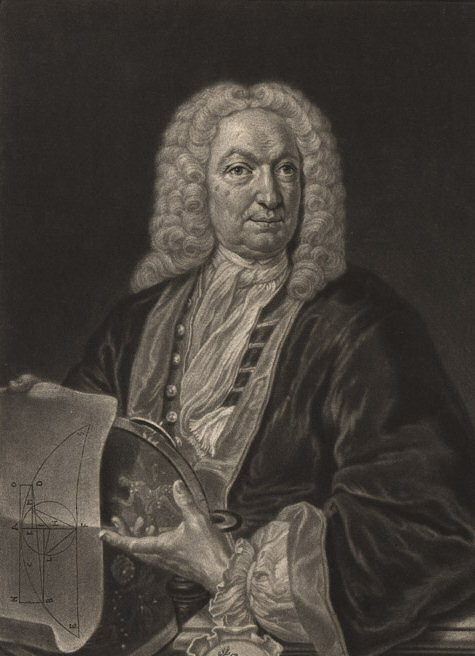
\includegraphics[width=0.28\textwidth]{assets/lectures-11609b3d.png} & 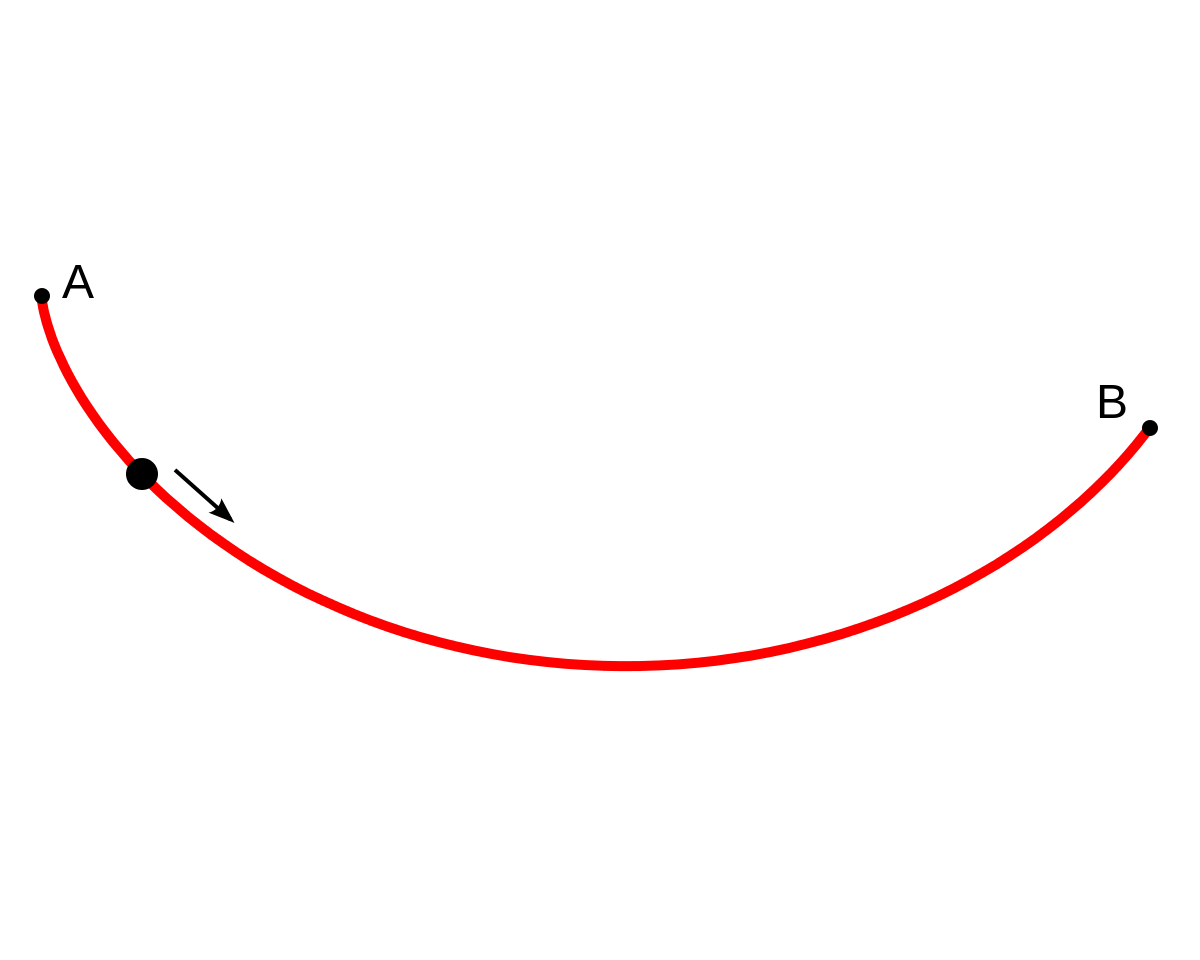
\includegraphics[width=0.6\textwidth]{assets/lectures-f1089691.png}\\
\text{Йоганн Бернуллі} & \text{Іллюстрація задачі ''задачі про брахісторону''}
\end{array}
$$
\textbf{Задача: } задано дві точки $A$ та $B$ на полощині, які не лежать на вертикальній прямій. Знайти гладку криву, по якій матераільна точка лише під дією сили тяжніння скотиться з точки $A$ в точку $B$ за найкоротший проміжок часу. \par Протягом року Йоганн Бернуллі розв'язав задачу сам і отримав ще чотири різних ров'язки від Ісаака Ньютона, Якоба Бернуллі, Готфріда Вільгельма Лейбніца, Гійома де Лопіталя. І саме розв'язання задачі про брахісторону, запропоноване Ісааком Ньютона, дало початок розвитку варіаційного числення як окремої матетматичної теорії. В подальшому варіаціїне числення завдячує своєму розвитку таким вченим як Леонард Ейлер, Жозеф Луі Лагрнаж, Карл Якобі, Адрієн-Марі Лежандр, Карл Вейєрштрасс та інші.\par

Нехай $Y$ -- дійсний нормований простір з нормою $||y||$ елементів $y \in Y$

\begin{example}
  $C[a, b]$ -- дійсний нормований простір з нормою: $$||\varphi(x)||_{C[a, b]} = \max\limits_{x \in [a, b]}|\varphi(x)|$$
  Нехай $M \subset Y$ -- деяка підмножина. Відображення $F: M \rightarrow \mathbb{R}; M \subset Y$ називається функціоналом з областью визначення $M$. Тобто на множині $M \subset Y$ задана функціонал $F(y)$, якщо кожному елементу $y \in M$ однозначно поставлено у відповідність дійсне число.
\end{example}
\begin{example}
  $J(y) = \mathop{\mathlarger{\int}}\limits_{a}^{b}y(x)\mathrm{d}x, \quad a, b \in \mathbb{R}, \quad a < b$, що розглядаютсья на множині функцій $M = \{ y \in C[a,b] \  | \  y(a) = A, \ y(B) = B\}$ є функціоналом, який кожній функції з множини $M$ ставить у відповідність значення інтеграла.
\end{example}
Класичне варіаційне числення вивчає загальні методи знаходження екстремумів функціоналів, заданих в певних функціональних просторах.

\subsection{Найпростіша задача варіаційного числення}
Розглянемо $C^1[a, b]$ -- дійсний нормований простір з нормою:
$$||\varphi(x)||_{C^1[a, b]} = \max\limits_{x \in [a, b]}|\varphi(x)| + \max\limits_{x \in [a, b]}|\varphi'(x)|$$
Нехай $a, b \in \mathbb{R}, \ a < b$ -- задані числа. $F(x, y, p) \in C^1([a, b] \times \mathbb{R}^2)$ -- задана функція. Розглянемо інтеграл:
\begin{equation}\label{varcalc_f1}
  J(y) = \mathop{\mathlarger{\int}}\limits_{a}^{b}F(x, y(x), y'(x))\mathrm{d}x
\end{equation}

На множині функцій:
$$M = \{ y \in C^1[a, b] \  | \  y(a) = A, \ y(b) = B\}$$
 де числа $A, B \in \mathbb{R}$ -- задані. Функції $y \in M$ називаються допустимими. \\
 Тоді $J(y)$ --- \textbf{функціонал} на $M$.

\defo Допустима функція $\tilde{y}(x) \in M$ дає слабкий локальний мінімум (максимум) функціоналу $J(y)$ на $M$, якщо $\exists \delta > 0 : \forall y \in M :|| y - \tilde{y}||_{C^1[a,b]} < b$ справедливо, що: $J(y) \geq (\leq) J(\tilde{y})$.

\defo Допустима функція $\tilde{y}(x) \in M$ дає слабкий глобальний мінімум (максимум) функціоналу $J(y)$ на $M$, якщо  $J(y) \geq (\leq) J(\tilde{y})$.

\defo Задача пошуку слабкого локального (глобального) екстремуму (min, max) функціоналу $J(y)$ на $M$ називається найпростішою задачею варіаційного числення.

Відомо, що при дослідженні функцій на екстремум вирішальну роль відіграє похідна функції. При дослідженні екстремумів функціоналів схожу роль відіграє поняття варіації функціоналу. Введемо його.

Для довільної функції $y \in M : \forall h(x) \in C^1[a, b]$ такої, що $h(a) = h(b) = 0$ та $\forall \alpha \in \mathbb{R}$ розглянемо сімейство функцій: $$y(x, \alpha) = y(x) + \alpha h(x)$$
Тоді $\forall \alpha \in \mathbb{R} y(x, \alpha) \in M$ розглянемо: $$ J(y + \alpha h) = \int\limits_{a}^{b} F(x, y(x) + \alpha h(x), y'(x) + \alpha h'(x)) \mathrm{d}x$$

Тоді функція $\Phi(\alpha) := J(y + \alpha h)$ є неперервно-диференційовную по $\alpha$ в деякому околі точки $\alpha = 0$.

$$\Phi'(0) = \dfrac{\mathrm{d}}{\mathrm{d}\alpha}J(y + \alpha h)\Big|_{\alpha = 0} = \int\limits_{a}^{b}\left(\dfrac{\partial F(x, y, y')}{\partial y} \cdot h(x) + \dfrac{\partial F(x, y, y')}{\partial y'} \cdot h'(x)\right)\mathrm{d}x$$

\defo Допустимим приростом (варіацією) функції $y \in M$ називають довільну функцію $h(x) \in C^1[a, b] : h(a) = h(b) = 0$.

Вираз $\ \dfrac{\mathrm{d}}{\mathrm{d}\alpha} J(y + \alpha h)\Big|_{\alpha = 0}$, де $h(x)$ -- допустимий приріст, називають першою варіацією функціоналу $J(y)$ на функції $y(x)$ в напрямку $h(x)$, позначення:

$$ \delta J(h, y) =  \dfrac{d}{d\alpha} J(y + \alpha h)\Big|_{\alpha = 0}$$

\begin{boxteo}
  Нехай $\tilde{y}(x) \in M$ --  розв'язок найпростішої задачі варіаційного числення. Тоді:
% \vspace{-2em}
  $\delta J(\tilde{y}, h) = 0 \ \ \forall h \in C^1[a, b] : h(a) = h(b) = 0$.
\end{boxteo}

\begin{proof}
  Нехай $\tilde{y}(x) \in M$ дає слабкий локальний мінімум задачі, тобто $$\exists \delta > 0 : \forall \eta \in C^1[a, b] : \eta(a) = \eta(b) = 0 : ||\eta||_{C^1[a,b]} < \delta$$ справедливо, що $J(\tilde{y} + \eta) \geq J(\tilde{y})$. Покладемо: $$\eta(x) = \alpha h(x), \ \text{де } h(x) \text{ --- допустимий приріст.}$$
  Тоді $\tilde{y} = \eta \in M$ та для достатньо малих $\alpha$:
  $$
  ||\eta|| = |\alpha| \left( \max\limits_{x\in [a,b]} \left| h(x) \right| + \max\limits_{x\in [a,b]} \left| h'(x) \right| \right) = |\alpha| \cdot ||h||_{C^1[a,b]} < \delta
  $$
  Таким чином:
  $
  \Phi(\alpha) = J( \tilde{y} + \alpha h) \geq J  (\tilde{y}) = \Phi(0) \
  $
  $\Longrightarrow$ точка $\alpha = 0 $ --- точка локального мінімуму $\Phi (\alpha). $ Тому:
  $
  0 = \Phi'(0) = \delta J(\tilde{y}, h)
  $
\end{proof}

\begin{remark}
  Дана теорема є незручною для розв'язання задач. Для того, щоб встановити більш зручну теорему, потрібна \textit{Лема Лагранжа}.
\end{remark}

\begin{boxlema}
  Якщо $f\in C[a,b]$ і $ \int\limits_{a}^{ b}{f(x)h(x) \mathrm{d}x} =0\ :\
  \forall h \in C^1[a, b] : h(a) = h(b) = 0
  $, тоді: $f(x) = 0 \ \ \forall x \in [a,b]$.
\end{boxlema}

\begin{proof}
 Припустимо від супротивного, що $\exists x_0 \in [a,b] : f(x_0) \neq 0.$ Візьмемо $f(x_0)>0$. Оскільки $f \in C[a,b]$, то існує окіл цієї точки: $$O_{\varepsilon } (x_0) = (x_0 - \varepsilon , x_0 + \varepsilon) \text{ такий, що: } f(x) > 0 \ \forall x \in O_{\varepsilon}(x_0) $$  Візьмемо:
 $$
 h(x) = \begin{cases}
  (x-(x_0 -\varepsilon ))^2(x-(x_0 +\varepsilon ))^2, & x \in O_{\varepsilon};\\
  0,  & x \notin O_{\varepsilon}.
 \end{cases} \quad \begin{gathered}
  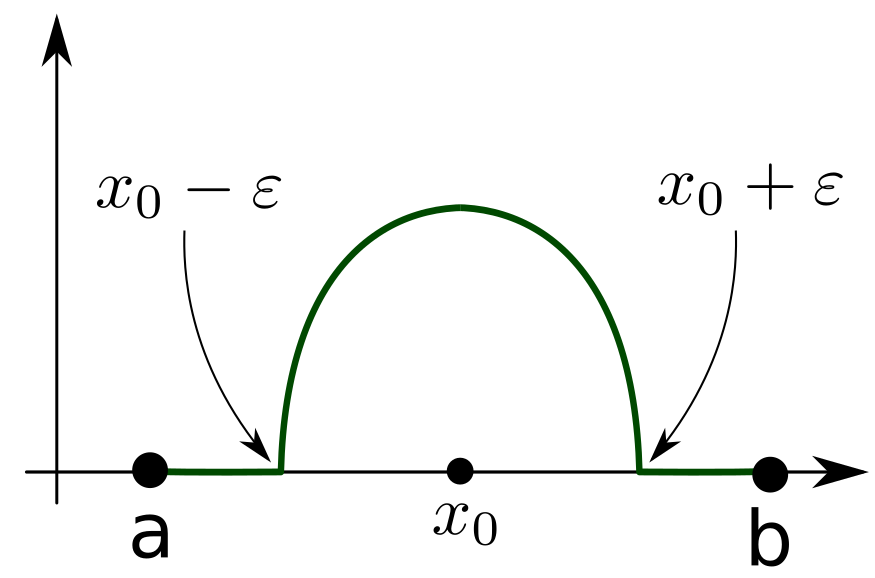
\includegraphics[scale=0.17]{assets/lectures_recent-91d0043b.png}
 \end{gathered}
 $$
 Тоді $h(x) \in C^1 [a,b], h(a) = h(b) = 0$. При цьому:
 $$
 0 =  \int\limits_{a}^{b}{f(x)h(x) \mathrm{d}x} =  \int\limits_{x_0 + \varepsilon}^{ x_0 - \varepsilon}{\underbrace{f(x) h(x)}_{ > 0 \text{ за прип.}}\mathrm{d} x } > 0
 $$
 Отримали протиріччя $0 > 0$.
\end{proof}

\begin{boxteo}
 Нехай $F(x,y,p)  \in C^2([a,b] \times \mathbb{R}^2)$ -- задана функція. Нехай допустима функція $\tilde{y} \in C^2[a,b]$ є розв'язком найпростішої задачі варіаційного числення. Тоді $\tilde{y}(x)$ задовільняє рівняння Ейлера на $[a,b]$:
 $$
 \frac{\d F}{\d y} - \frac{\mathrm{d} }{\mathrm{d} x} \frac{\d F}{\d y'} =0
 $$
\end{boxteo}

\begin{proof}
Нехай  $\tilde{y} \in C^2[a,b]$ є розв'язком найпростішої з.в.ч. Тоді:
$$
\delta J(\tilde{y}, h) = 0 \qquad \forall h \in C^1 [a,b] : h(a) = h(b) = 0
$$
$$
0 = \delta J(\tilde{y}, h) = \frac{\mathrm{d}}{\mathrm{d}\alpha} J(\tilde{y} + \alpha h) \vline_{\alpha=0} =
  \int\limits_{a}^{b}{ \frac{\d F}{\d y} (x, \tilde{y}, \tilde{y}') \cdot h(x) + \frac{\d F}{\d y'} (x, \tilde{y}, \tilde{y}') \cdot h'(x)
 } =$$$$= \left|
\begin{gathered}
 u =   \frac{\d F}{\d y'} (x, \tilde{y}, \tilde{y}')\\
 du = \frac{\mathrm{d} }{\mathrm{d} x} \left(  \frac{\d F}{\d y'} (x, \tilde{y}, \tilde{y}') \right)
\end{gathered} \ \
\begin{gathered}
 dv = h' (x ) \mathrm{d}x \\
 v = h(x)
\end{gathered}
  \right| =   \int\limits_{a}^{b}{ \frac{\d F}{\d y} (x, \tilde{y}, \tilde{y}') \cdot h(x) \mathrm{d}x} \ +
$$
$$
+ \underbrace{ \left. \frac{\d F}{\d y'} (x, \tilde{y}, \tilde{y}') \cdot h(x) \right|_{a}^b}_{ = 0 \ \Leftarrow \ h(b) = h(a) = 0}  -  \int\limits_{a}^{ b}{\frac{\mathrm{d} }{\mathrm{d} x} \left(  \frac{\d F}{\d y'} (x, \tilde{y}, \tilde{y}') \right) \cdot h(x) \mathrm{d} x} =
$$
$$
 =  \int\limits_{a}^{b}{ \left[
 \frac{\d F}{\d y} (x, \tilde{y}, \tilde{y}')
  - \frac{\mathrm{d} }{\mathrm{d} x} \left(  \frac{\d F}{\d y'} (x, \tilde{y}, \tilde{y}') \right)
  \right]\cdot h(x) \mathrm{d} x} = 0
$$
$$
\forall h \in C^1[a,b] : h(a) = h(b) = 0 \xRightarrow{\text{лема Лагранжа}} \text{ рівняння Ейлера.}
$$
\end{proof}

\begin{defo}
  Розв'язки рівняння Ейлера називаються \textbf{екстремалями} функціоналу $J(y)$. Екстремалі, які є допустимими функціями, називаютсья \textit{допустимими екстремалями}. Саме серед допустимих екстремалей слід шукати розв'язок НЗВЧ.
\end{defo}
\begin{remark}
  Умови $\tilde{y} \in C^2[a,b] , F\in C^2 \left( [a,b] \times \mathbb{R}^2 \right)$ накладені з метою спростити доведення (щоб ''узаконити'' інтегрування частинами). Насправді, твердження теореми буде вірним і для неперервно-диференційованих функцій.
\end{remark}


\begin{example}
 $$
 \begin{dcases}
   \int\limits_{0}^{ 1}{(y'(x))^2 \mathrm{d} x} \to \mathrm{extr};\\
   y(0) = 0 \qquad y(1) = 1.
 \end{dcases}
 $$
 \begin{enumerate}
   \item Складаємо і розв'язуємо рівняння Ейлера:
   $$
   \frac{\d F}{\d y} - \frac{\mathrm{d} }{ \mathrm{d} x} \frac{\d F}{\d y'} = 0
   $$
   $$
   F(x,y,y') = (y')^2 \qquad \frac{\d F}{\d y} = 0 \qquad \frac{\d F}{\d y'} = 2y'
   $$
   $$
   \frac{\mathrm{d}}{\mathrm{d} x} \frac{\d F}{ \d y'} = \frac{\mathrm{d}}{\mathrm{d} x} (2 y') = 2 y''  \ \Longrightarrow \
   0 - 2y'' = 0 \ \Longrightarrow \  \fbox{$y'' = 0$}
   $$
   Отримали рівняння Ейлера. Двічі інтегруємо:
   $$
   y = C_1 x + C_2 \text{ --- сімейство екстремалей.}
   $$
   \item Знаходимо допустимі екстремалі.
   $$
   y(0) = 0 \ \Rightarrow \  0 = C_1 \cdot 0 + C_2 \ \Rightarrow \  C_2 = 0
   $$
   $$
   y(1) = 1 \ \Rightarrow \  1 = C_1 \cdot 1 \ \Rightarrow \  C_1 = 1
   $$
   $$
   \tilde{y}(x) = x \text{ --- допустима екстремаль.}
   $$
   \item Перевіряємо, чи досягаєтся в $\tilde{y} (x)\  \mathrm{extr}$ функціоналу $J(y)$:\\
   $
   \forall h \in C^1 [0,1] : h(0) = h(1) = 0
   $ розглядаємо $J(\tilde{y} + h) - J(\tilde{y})$.\\
 \end{enumerate}
 \begin{itemize}
   \item    Якщо $J(\tilde{y}+ h) - J(\tilde{y})  \geq 0 \ \ \forall h \in C^1 [0,1] : h(0) = h(1) = 0$  принаймі з деякого околу $||h||_{C^1 [0,1]} < \delta$, то $\tilde{y} (x) $ забезпечує слабкий локальний мінімум функціоналу.
   \item Якщо $J(\tilde{y}+ h) - J(\tilde{y})  \geq 0 \ \ \forall h \in C^1 [0,1] : h(0) = h(1) = 0$, то $\tilde{y} (x) $ забезпечує слабкий глобальний мінімум функціоналу.
   \item Якщо нерівність виконується з протилежним знаком ($ \leq 0$), то досягається максимум (локальний або глобальний).
   \item Якщо різниця функціоналів знакозмінна, то extr не досягається.
 \end{itemize}
 Маємо:
 $$
 J(\tilde{y} + h) - J(\tilde{y}) =  \int\limits_{0}^{1}{ (\tilde{y}' + h')^2 \mathrm{d}x} -  \int\limits_{0}^{ 1}{ (\ty')^2 \mathrm{d} x} =
 $$
 $$
 =  \int\limits_{0}^{ 1}{ (\ty')^2  + 2 \ty'h' + h'^2  -  (\ty')^2 \mathrm{d}x} \oeq
 $$
 $$
 \left(  \int\limits_{0}^{1}{ \ty' h'} =  \left|  \begin{gathered}
  \ty' = u\\
  \ty'' = \mathrm{d}u
 \end{gathered}\ \ \begin{gathered}
  h' = v' \\
  h = v
 \end{gathered} \right| = \ty' h\bigg|_0^1 -  \int\limits_{0}^{1}{ \ty'' h \mathrm{d}x} = 0 \right)
 $$
 $$
 \oeq  \int\limits_{0}^{1}{ (h')^2 \mathrm{d}x} \geq  \quad \forall h \in C^1[0,1] : h(0) = h(1) = 0 \Longrightarrow \fbox{сл. глобальний мінімум.}
 $$
\end{example}

\begin{example}
 $$
 \begin{dcases}
  J(y) =  \int\limits_{0}^{1}{ (y + y')^2 \mathrm{d} x} \to \mathrm{extr}\\
  y(0) = 1 \qquad y(1) = 0
 \end{dcases}
 $$
\end{example}
\begin{enumerate}
  \item Складаємо і розв'язуємо рівняння Ейлера:
  $$
  F = (y + y')^2 \qquad \frac{\d F}{\d y} = 2(y + y') \qquad \frac{\d F}{\d y'} = 2(y + y')
  $$
  $$
  \frac{\d F}{\d y} - \frac{\mathrm{d} }{\mathrm{d}x } \frac{\d F}{\d y'} = 0, \ \ y + y' - \frac{\mathrm{d} }{\mathrm{d} x} (y + y') = 0
  $$
  $$
  y + y' - y' - y'' = 0 \ \ \Longrightarrow \ \  y'' - y = 0  \textit{ --- рівняння Ейлера.}
  $$
  Отримали ЛОР 2-го порядку. Складемо характеристичне рівняння:
  $$
  \lambda^2 - 1 = 0 \ \Longrightarrow \  \lambda= \pm 1 \ \Longrightarrow \  y(x) = C_1 + e^x + C_2 e^{-x} \text{-- сімейство екстремалей.}
  $$
  \item Знаходимо допустові екстремалі:
  $$
  \begin{array}{l c c c}
    y(0) = 1 : & 1 = C_1 e^0 + C_2 e^0  & \Longrightarrow & C_1 + C_2 = 1\\
    y(1) = 0 : & 0 = C_1 e^{1} + C_2 e^{-1}  & \Longrightarrow & C_1 + C_2e^{-2} = 0\\
  \end{array} \Rightarrow
  \begin{cases}
    C_1 + C_2 = 1\\
    C_1 + C_2e^{-2} = 0
  \end{cases}
  $$
  $$
  C_2 (e - e^{-1}) = e  \quad  \Longrightarrow \quad C_2 = \frac{e}{e - e^{-1}}  \quad \Longrightarrow \quad C_1 = - \frac{1}{e ( e - e ^{-1})}
  $$
  $$
  \ty (x) =  - \frac{1}{e ( e - e ^{-1})}  e^{x} + \frac{e}{e - e^{-1}} e^{-x} = \frac{1}{e - e^{-1}}  \left(  - e^{x-1} + e^{-x +1} \right) = - \frac{\sh(x-1)}{\sh(1)}
  $$
  Отримали $- \frac{\sh(x-1)}{\sh(1)}$ --- допустима екстремаль.
  \item Перевірка. Перевіряємо, чи забезпечує $\ty (x) $ екстремум задачі.\\
  $
  \forall h \in C ^1 [0,1] : h(0) = h(1) = 0:
  $
  $$
  J(\ty  + h ) - J(\ty) =  \int\limits_{0}^{1}{ ((\ty + h) + (\ty' + h'))^2 \mathrm{d}x} -  \int\limits_{0}^{1}{
  (\ty + \ty')^2 \mathrm{d}x
  } =
  $$
  $$
  =  \int\limits_{0}^{1}{ (\ty + h)^2 + 2 (\ty + h) (\ty' + h') + (\ty' + h')^2 \mathrm{d} x} -  \int\limits_{0}^{1}{ \ty^2 + 2 \ty\ty' + (\ty')^2 \mathrm{d}x} =
  $$
  $$
  = \left|  \textit{розкриваючи дужки} \right| =  \int\limits_{0}^{1}{ h^2 + (h')^2 + 2 (\ty + \ty') h + 2(\ty + \ty')h' \mathrm{d} x } \oeq
  $$
  $$
  \left( \begin{gathered}
   \text{ Візьмемо частинами:} \\
 \int\limits_{0}^{1}{ (\ty + \ty')h' \mathrm{d}x} = \left|  \begin{gathered}
  (\ty + \ty') = u \\
  (\ty' + \ty'' ) = \mathrm{d} u
 \end{gathered} \ \begin{gathered}
  h' = v' \\
  h = v
 \end{gathered} \right| = \ \\
 = \underbrace{(\ty + \ty')h \bigg|_{0}^{1}}_{ = 0 \ \Leftarrow \ h(0)=h(1)=0 } -  \int\limits_{0}^{1}{(\ty' + \ty'' )h \mathrm{d}x}
  \end{gathered} \right)
  $$
  $$
  \oeq  \int\limits_{0}^{1}{h^2 + (h')^2 + \underbrace{2 (\ty + \ty' - \ty' - \ty'')}_{=0 \ \Leftarrow \ \ty = \ty'' (\text{з р-ня Ейлера})h} \mathrm{d}x} =
  $$
  $$
  =  \int\limits_{0}^{1}{ (h^2 + (h')^2)\mathrm{d}x} \geq 0 \qquad
   \forall h \in C^1[a,b] : h(0) = h(1) = 0
  $$

  Отримали: \fbox{$\ty(x) = -\frac{\sh(x-1)}{\sh(1)} $ --- слабкий глобальний мінімум функціоналу.}
\end{enumerate}

\subsection{Задача про брахісторону}
Знайти криву, по якій матеріальна точка скотиться найшвидше, нехтуюч тертям та опорою середовища.
Нехай $A$ - точка початку координат, т. $B (x_1, y_1)$.
$$
\begin{gathered}
 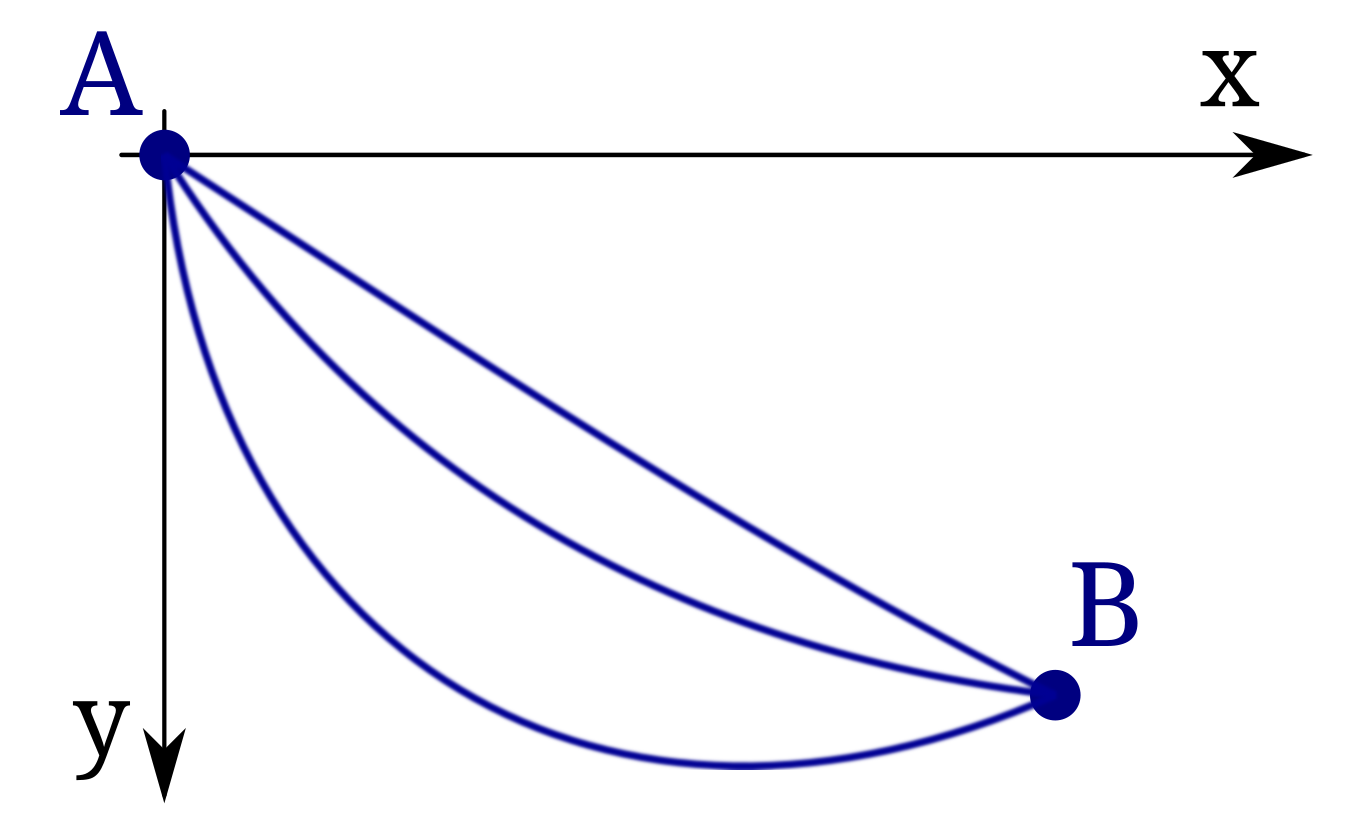
\includegraphics[scale=0.2]{assets/lectures_part_3-91d0349d.png}
\end{gathered}
\qquad \quad
\begin{gathered}
U(x) = \frac{\mathrm{d} s}{ \mathrm{d} t} \ \Longrightarrow \ \mathrm{d}t = \frac{\mathrm{d} s}{U(x)}\\
\mathrm{d} s = \sqrt{1 + (y')^2} \mathrm{d} x\\
\text{Закон збереження енергії:}\\
\frac{mv^2}{2} = mgy \ \Longrightarrow \  v = \sqrt{2gy} \\
\mathrm{d}t = \dfrac{\sqrt{1 + (y')^2} \mathrm{d} x}{\sqrt{2gy}}
\end{gathered}
$$
Отримали математичну постановку задачі:
$$
\begin{dcases}
 t = \frac{1}{2g}  \int\limits_{0}^{x_1}{ \sqrt{ \frac{1+ (y')^2}{y} } \mathrm{d} x} \to \mathrm{extr}\\
 y(0) = 0 \qquad \quad y(x_1)  = y_1
\end{dcases}
$$
Класичне рівняння Ейлера надто складне для даної задачі.
\begin{boxlema}
  Якщо $F(x,y,y') = F(y, y')$, то рівняння Ейлера набуває наступного вигляду:
  $$
  \frac{\mathrm{d}}{\mathrm{d} x} \left( F - y' \frac{\d F}{ \d y'}  \right) = 0
  $$
\end{boxlema}
\begin{proof}
 Розглядаємо рівняння Ейлера:
 $$
 \frac{\d F}{\d y} - \frac{\mathrm{d} }{\mathrm{d} x} \left( \frac{\d F}{\d y'}  \right) = 0
 $$
$$
{ \everymath={\displaystyle}
\begin{array}{c c l}
\frac{\mathrm{d}}{\mathrm{d} x} \left( F (y, y') - y' \frac{\d F}{\d y}  \right) & = &\frac{\d F}{\d y} \cdot y' +
\frac{\d F}{\d y} \cdot y'' - y'' \frac{\d F}{\d y} - y' \frac{\mathrm{d}}{\mathrm{d} x} \left( \frac{\d F}{\d y'}  \right) =\\
\  & = & 0 + y'  \underbrace{\left(\frac{\d F}{\d y} - \frac{\mathrm{d} }{\mathrm{d} x} \left( \frac{\d F}{\d y'}  \right)  \right)}_{=0}   = 0
\end{array}}
 $$
\end{proof}

$$
\frac{\mathrm{d} }{\mathrm{d} x} \left( F  - y' \frac{\d F}{\d y'}  \right) = 0 \quad \Longrightarrow \quad
F - y' \frac{\d F}{\d y'} = C \quad \Longrightarrow \quad F = \sqrt{ \frac{1 + (y')^2}{y} }
$$

$$
\frac{\d F }{\d y'} = \frac{1}{\sqrt{y}} \cdot \frac{2 y'}{2 \sqrt{1 + (y')^2}}  = \frac{y'}{\sqrt{y (1 + y')^2}}
$$
Маємо:
$$
\sqrt{ \frac{1 + (y')^2}{y} } - \frac{(y')^2}{\sqrt{y (1 + y')^2}} = C
$$
Домножимо ліву та праву і праву частину на $\sqrt{y(1 + (y')^2)}$:
$$
1 + (y')^2  - (y')^2 = C \sqrt{y(1 + (y')^2)}, \ \ y(1 + (y')^2) = C_1 \text{, де } C_1 = \frac{1}{C^2}
$$
Отримали рівняння, нерозв'язне відносно похідної:
$$
y = \frac{C_1}{ 1 + (y')^2}
$$
Параметризація:
$$
x = x \qquad y' = \ctg{p} \qquad p\text{ -- параметр}, \  y = \frac{C_1}{ 1 + \ctg^2{p}} = C_1 \cdot \sin^2{p}, \  dy = y'dx
$$
$$
2 C_1 \sin{p} \cos{p} \mathrm{d} p = \frac{\cos{p}}{\sin{p}} \mathrm{d}x, \ \ 2 C_1 \sin^2{p} \mathrm{d} p = \mathrm{d}x, \ \ C_1 (1 - \cos{( 2p)})  \mathrm{d} p = \mathrm{d} x
$$
$$
\begin{dcases}
 x = C_1 ( p - \frac{ \sin{(2p)}}{2} ) + C_2\\
 y = C_1 \sin^2{p}
\end{dcases}
\quad \Longrightarrow \quad
\begin{dcases}
 \text{Параметризоване рівняння циклоїди:}\\
 x = \frac{C_1}{2}  ( 2p - \sin{(2p)} ) + C_2\\
 y = \frac{C_1}{2} ( 1 - \cos{(2p)})
\end{dcases}
$$

Оскільки $y(0) = 0 \Longrightarrow C_2 = 0$. $C_1$ знаходимо з умови $y(x_1) = y_1$.


\section{Лекція 7}
\subsection{Задча з вільним кінцем}
Нехай $a, b \in \mathrm{R}, a < b$ -- задачі числа, $F(x, y, p) \in C^2([a, b] \times \mathrm{R}^2)$ -- задана функція. Розглянемо інтеграл: $$J(y) = \int\limits_{a}^{b}F(x, y(x), y'(x))\mathrm{d}x$$
На множині функцій: $$ M = \{ y \in C^1[a, b] \ | \ y(a = A)\}, \text{ де } A \in \mathrm{R} \text{ -- задане число} $$
Функції $y \in M$ -- допустимі функції.

\defo Допустима фунція $\tilde{y}(x) \in M$ забезпечує слабкий локальний min(max) функціоналу $J(y)$ на $M$, якщо $\exists \delta > 0 : \forall y \in M ||y - \tilde{y}||_{C^1[a, b]} < \delta$ справедливо, що $J(y) \geq (\leq) J(\tilde{y})$. Якщо нерівність виконується для $\forall y \in M$, то допустима функція $\tilde{y} \in M$ забезпечує глобальний min(max) функціоналу $J(y)$ на $M$.

\defo Задач пошуку слабкого локального (глобального) екстремуму функціоналу $J(y)$ на $M$ називається задачею з вільним кінцем.
 %

$$
\left[ \begin{array}{l}
    \dfrac{dv}{du} = \dfrac{\lambda_2}{\lambda_1} \cdot \dfrac{u}{v}\\
    u = 0
\end{array} \right.
\Longleftarrow
\begin{cases}
    \dot{u} = \lambda_1 u \\
    \dot{v} = \lambda_2 v
\end{cases} \Longrightarrow
\begin{cases}
    u = c_1 \cdot e^{\lambda_1 t}\\
    v = c_2 \cdot e^{\lambda_2 t}
\end{cases}
$$
Поділили двуге рівняння на перше, щоб вилучити $t$.
$$
\left[ \begin{array}{l}
    \dfrac{dv}{du} = \dfrac{\lambda_2}{\lambda_1} \cdot \dfrac{u}{v}\\
    u = 0
\end{array} \right. \Longrightarrow \left[ \begin{array}{l}
    \ln{ \left| v \right| } = \dfrac{\lambda_2}{\lambda_1} \ln{ \left| u \right| } + \ln{ \left| c \right| } \\
    u = 0, v = 0
\end{array} \right. \Longrightarrow
\left[ \begin{array}{l}
    v = c  \cdot u^{ \frac{\lambda_2}{\lambda_1} }\\
    u = 0, v = 0
\end{array} \right.
$$

Якщо $ \lambda_1 \cdot \lambda_1 > 0 $ та $ \left| \lambda_2 \right| > \left| \lambda_1 \right|  $ (стрілки від нуля за умови $
 \lambda_1, \lambda_2 > 0$):

\begin{center} 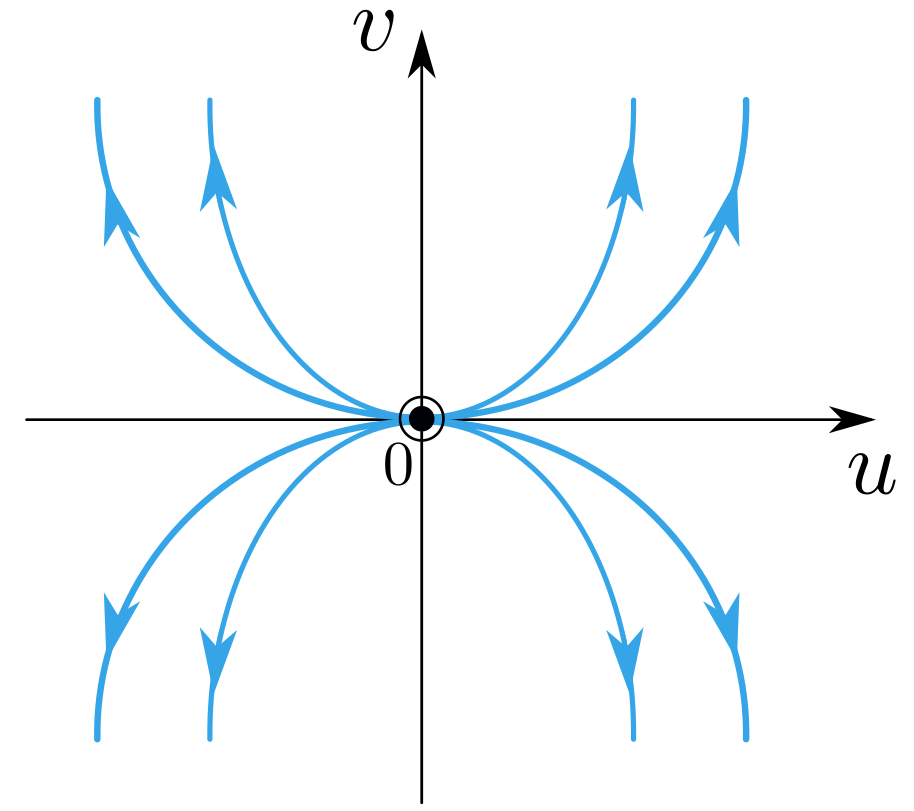
\includegraphics[scale=0.3]{assets/lectures_recent-b13d607a.png} \end{center}

Якщо $ \lambda_2 \cdot \lambda_1 > 0$ та  $ \left| \lambda_2 \right| > \left| \lambda_1 \right|  $ (стрілки до нуля за умови $
 \lambda_1, \lambda_2 < 0$):

 \begin{center} 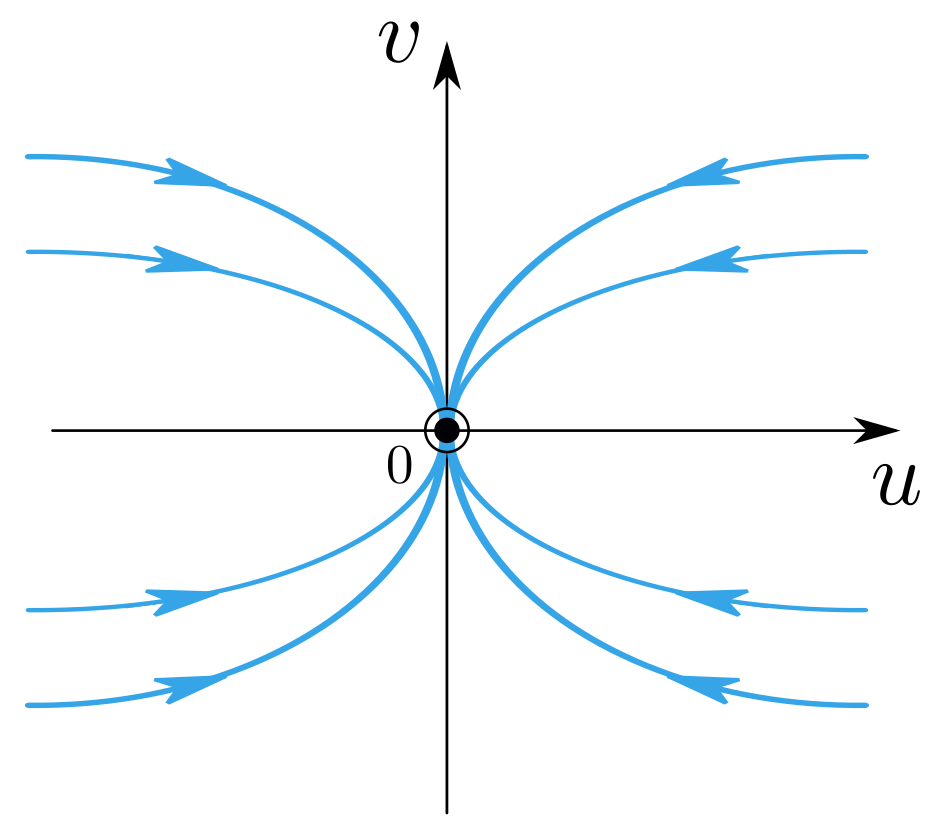
\includegraphics[scale=0.3]{assets/lectures_recent-392ff5ad.png} \end{center}

 Відмітимо, що якщо $\lambda_1, \lambda_2 < 0$, то напрям руху (по $t$) вздовж траєкторій відбувається до нуля. Якщо ж $\lambda_1, \lambda_2 >0$, то рух спрямовано від нуля.\\

 Залишається перейти до початкових змінних $ \begin{bmatrix}
  x \\
   y
 \end{bmatrix}$.\\
Таким чином, якщо $\lambda_1 , \lambda_2 \in \mathbb{R}, \lambda_1 \neq \lambda_2, \lambda_1 \cdot \lambda_2 > 0$ (власні числа одного знаку), то фазовий портрет має вигляд:

\begin{center} 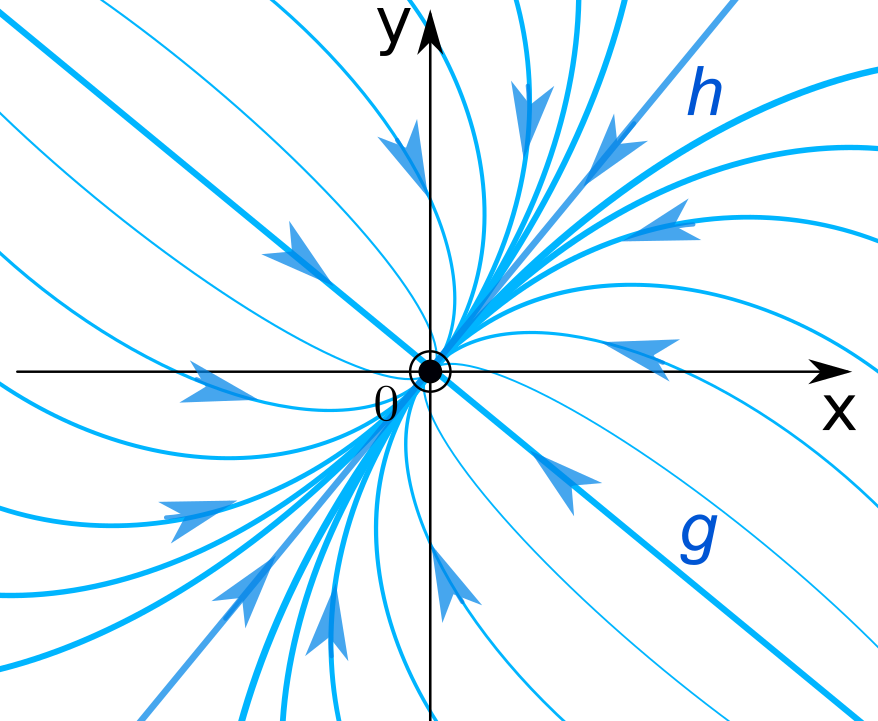
\includegraphics[scale=0.3]{assets/lectures_recent-deaf1762.png} \end{center}

На малюнку $h$ - пряма на якій лежить власний вектор, який відповідає меншому за модулем власному числу.\\
Такий фазовий портрет \textbf{вузол.}\\
- Якщо $\lambda_1, \lambda_2 > 0$ - нестійкий вузол (стрілки від нуля).\\
- Якщо $\lambda_1, \lambda_2 < 0$ - ас. стійкий вузол (стрілки до нуля).

\begin{example}
    $$
    \begin{cases}
    \dot{x} = 2y - 3x\\
    \dot{y} = x - 4y
    \end{cases} \qquad A = \begin{bmatrix}
     -3 & 2 \\
     1 & -4
    \end{bmatrix}
    $$
    $$
    \det{A - \lambda I} = \begin{vmatrix}
      -3 - \lambda & 2 \\
      1 & -4 - \lambda
    \end{vmatrix}  = (-3-\lambda) (-4 - \lambda) -2 = \lambda^2 + 7 \lambda + 10 = 0
    $$
    $$
    \lambda_1 = -2 \qquad \lambda_2 = -5 \Rightarrow \text{ас. стійкий вузол.}
    $$
    Знаходимо власні вектори:\\
    $\lambda_1 = -2$:
    $$
    \begin{bmatrix}
     -1 & 2 \\
     1 & -2
    \end{bmatrix} \begin{bmatrix}
     h_1 \\
     h_2
    \end{bmatrix} = \begin{bmatrix}
     0 \\
     0
    \end{bmatrix} \qquad \begin{gathered}
     -h_1 + 2h_2 = 0\\
     h_1 = 2 h_2
    \end{gathered} \Rightarrow \overline{h} = \begin{bmatrix}
     2 \\
     1
    \end{bmatrix}
    $$
    $\lambda_2 = -5$
    $$
    \begin{bmatrix}
     2 & 2 \\
     1 & 1
    \end{bmatrix} \begin{bmatrix}
     g_1 \\
     g_2
    \end{bmatrix} = \begin{bmatrix}
     0 \\
     0
    \end{bmatrix}
    \qquad \begin{gathered}
     g_1 + g_2 = 0\\
     g_1 = - g_2
    \end{gathered} \Rightarrow \overline{g} = \begin{bmatrix}
     1 \\
     -1
    \end{bmatrix}
    $$

    \begin{center} 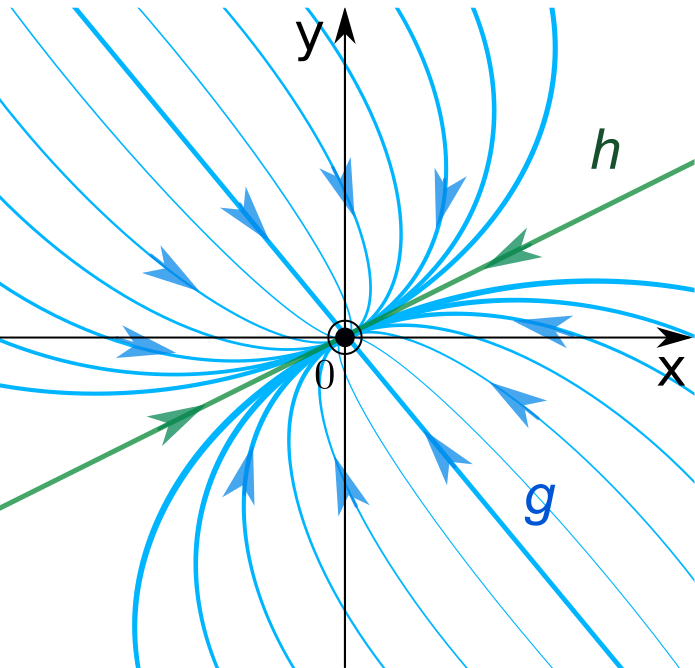
\includegraphics[scale=0.4]{assets/lectures_recent-06adae22.png} \end{center}
\end{example}

2. Нехай $ \lambda_1 , \lambda_2 \in \mathbb{R}, \lambda_1 \neq \lambda_2, \lambda_1 \cdot \lambda_2 < 0$ (Власні числа різних знаків).
Тоді, аналогічно, перейшовши до Жорданового базису, маємо:

$$
\begin{gathered}
\begin{cases}
    \dot{u} = \lambda_1 u\\
    \dot{v} = \lambda_2 v
\end{cases} \\ \begin{cases}
    u = c_1 \cdot e^{\lambda_1 t}\\
    v = c_2 \cdot e^{\lambda_2 t}
\end{cases} \\
 \left[ \begin{array}{l}
v = C \cdot u^{ \frac{\lambda_2}{\lambda_1} }\\
u =0 , v = 0
\end{array} \right.
\end{gathered}\quad
\begin{gathered} 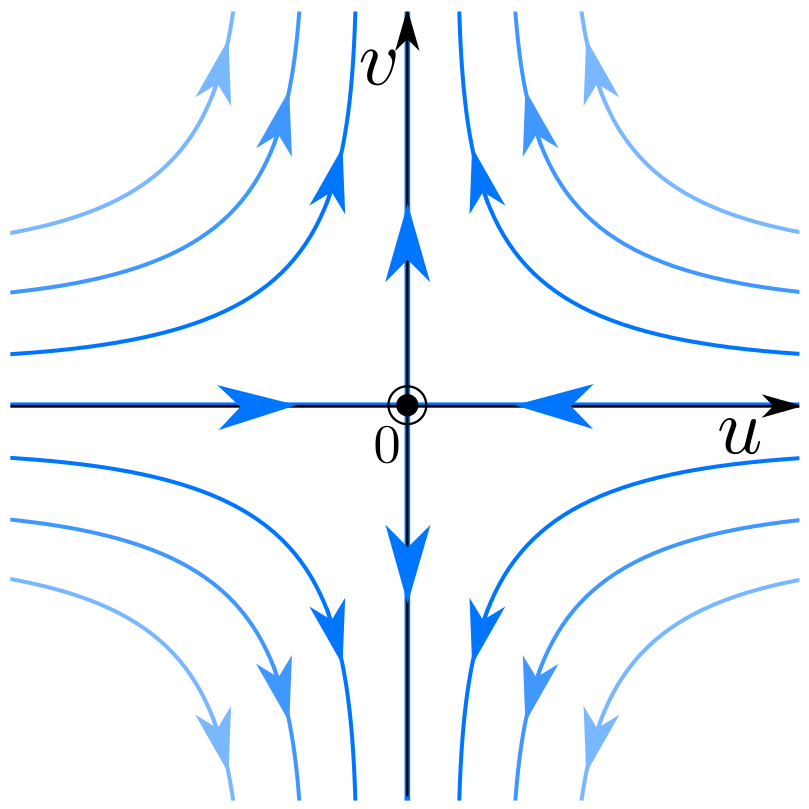
\includegraphics[scale=0.3]{assets/lectures_recent-53a0acd8.png} \end{gathered}
$$


Якщо $ \lambda_1 < 0,
  \lambda_2 > 0
$, то $
 \begin{gathered}
 u(t) \xrightarrow[t \to \infty]{} 0\\
 v(t) \xrightarrow[t \to \infty]{} \infty
 \end{gathered}.$\\
 Якщо $ \lambda_1 < 0,
  \lambda_2 > 0$, то  $
   \begin{gathered}
   u(t) \xrightarrow[t \to \infty]{} \infty\\
   v(t) \xrightarrow[t \to \infty]{} 0
   \end{gathered}.$\\
У другому випадку напрям руху траекторій відбуватиметься в інший бік.\\
Отже, перейшовши до початкових змінних, отримаємо, що за умови $\lambda_1 \cdot \lambda_2 < 0$ фазовий портрет має вигляд:

\begin{center} 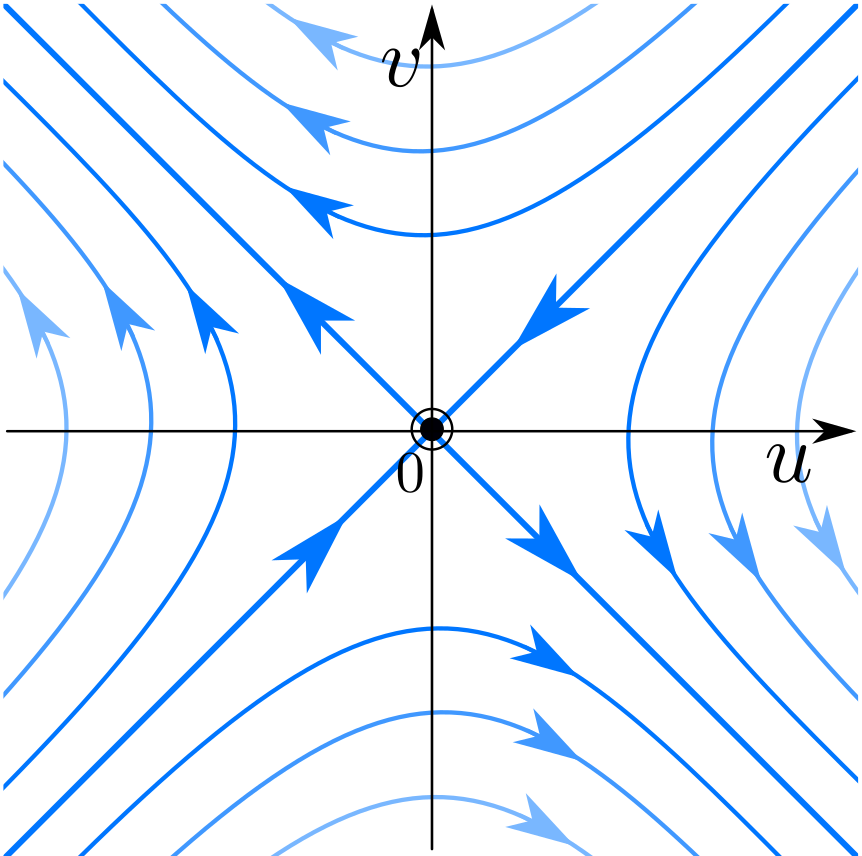
\includegraphics[scale=0.25]{assets/lectures_recent-0ebe704d.png} \end{center}

\begin{remark}
    Стрілки до нуля вздовж прямої, на якій лежить власний вектор, що відповідає $ \lambda_1 < 0$.\\
    Стрілки від нуля вздовж прямої, на якій лежить власний вектор, що відповідає $ \lambda_2 > 0$.
\end{remark}
Такий фазовий портрет називається \textbf{сідло}. Це завжди нестійке положення рівноваги.

\begin{example}
    $$
    \begin{cases}
        \dot{x} = x + 3y\\
        \dot{y} = 2x
    \end{cases} \qquad A = \begin{bmatrix}
     1 & 3 \\
     2 & 0
    \end{bmatrix}
    $$
    $$
    \det (A - \lambda I) = \begin{vmatrix}
      1-\lambda & 3 \\
      2 & - \lambda
    \end{vmatrix} = (1- \lambda)(-\lambda) - 6 = \lambda^2 - \lambda - 6 = 0
    $$
    $$
    \lambda_1 = 3 \quad \lambda_2 = -2 \Longrightarrow \text{сідло (нестійке)}
    $$
    Знаходимо власні вектори:
    $\lambda_1 = 3$
    $$
    \begin{bmatrix}
     -2 & 3\\
     2 & -3
    \end{bmatrix} \begin{bmatrix}
     h_1\\
     h_2
    \end{bmatrix} = \begin{bmatrix}
      0\\
      0
    \end{bmatrix} \qquad 2h_1 = 3 h_2 \Rightarrow \overline{h} = \begin{bmatrix}
     3 \\
     2
    \end{bmatrix}
    $$

    $\lambda_2 = -2$

    $$
    \begin{bmatrix}
     3 &3 \\
     2 & 2
    \end{bmatrix} \begin{bmatrix}
     g_1 \\
     g_2
    \end{bmatrix} = \begin{bmatrix}
     0 \\
     0
    \end{bmatrix} \qquad 2 g_1 =-2 g_2 \Rightarrow \overline{g} = \begin{bmatrix}
     1 \\
     -1
    \end{bmatrix}
    $$
    Отримали такий фазовий портрет:
    \begin{center} 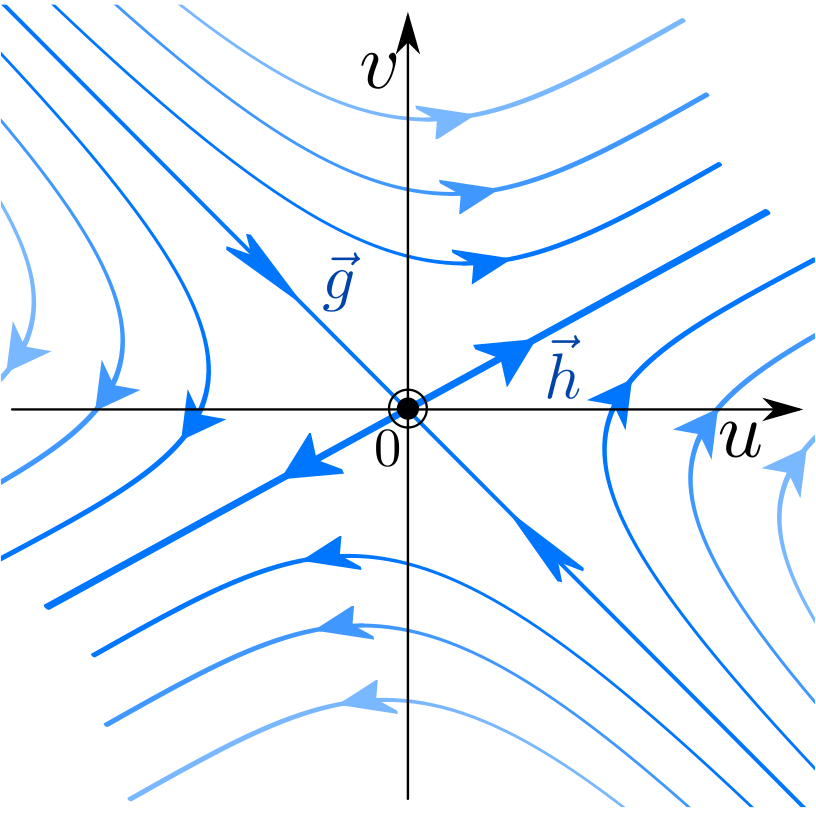
\includegraphics[scale=0.3]{assets/lectures_recent-c4b9c37b.png} \end{center}
    \end{example}


    3. Нехай $ \lambda_1 = \lambda_2 = \lambda \in \mathbb{R}$.\\
    a) Матриця $A$ - діагональна.
    $$
    A = \begin{bmatrix}
     \lambda & 0 \\
     0 & \lambda
    \end{bmatrix} \Longrightarrow \begin{cases}
        \dot{x} = \lambda x\\
        \dot{y} = \lambda y
    \end{cases}
    $$
    В такому випадку, фазовий портрет називають \textbf{диктричний вузол.}




\begin{center} 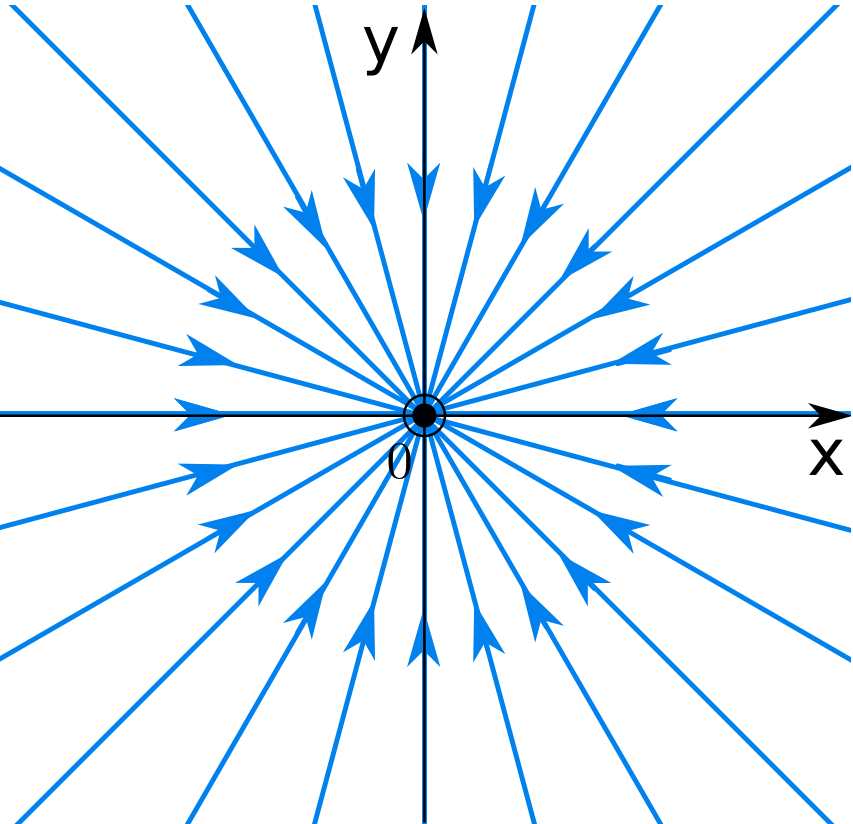
\includegraphics[scale=0.3]{assets/lectures_recent-ab36e3f3.png} \end{center}


Якщо $ \lambda < 0 $ - ас. стійкий (стрілки до нуля).\\
Якщо $ \lambda > 0 $ - нейстійкий (стрілки від нуля). \\
б) Матриця $A$ - недіагональна. В такому разі, фазовий портрет називають \textbf{вироджений вузол.}\\
- якщо $ \lambda < 0 $ - ас. стійкий ( стрілки до нуля ).\\
- якщо $ \lambda > 0 $ - нестійкий (стрілки від нуля).\\
Вироджений вузол може бути двох видів:
\begin{center} 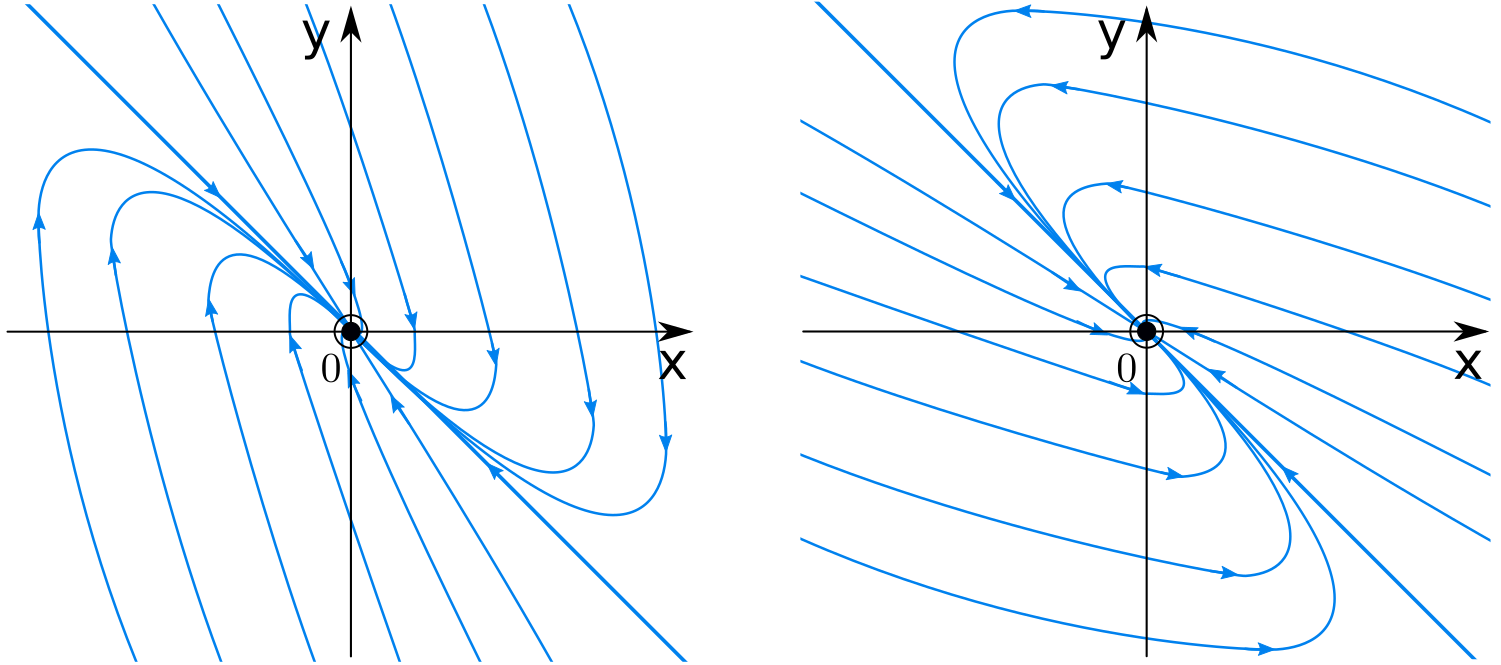
\includegraphics[scale=0.25]{assets/lectures_recent-b526bf37.png} \end{center}

Для визначення типу виродженого вузла потрібно визнгачити напрям вектора фазової швидкості $ \begin{bmatrix}
 \vec{x} \\
 \vec{y}
\end{bmatrix}$ в довільній точці, що не дорівнює нулю системи координат. Цей напрям має співпадати із напрямами руху по фазовій траєкторії (до нуля або від нуля).

\begin{example}
    $$
    \begin{cases}
        \vec{x} = 2y - 3x\\
        \vec{y} = y - 2x
    \end{cases} \qquad A = \begin{bmatrix}
     -3 & 2 \\
     -2 & 1
    \end{bmatrix}
    $$

    $$
    \det{ \left( A - \lambda I  \right) } = \begin{vmatrix}
      -3 - \lambda & 2 \\
      -2 & 1 - \lambda
    \end{vmatrix} = ( -3 - \lambda ) ( 1 -\lambda) + 4 =  \lambda^2 + 2 \lambda + 1 =
    $$
    $$
    = ( \lambda+ 1) ^2 = 0 \Longrightarrow  \lambda = -1 - \text{кратності 2. }
    $$
З попереднього випливає, що фазовим портретом буде асимптотично стійкий вироджений вузол (стрілки до нуля).
Знайдемо власний вектор:
$$
\begin{bmatrix}
 -2 & 2 \\
 2 & 2
\end{bmatrix} \begin{bmatrix}
 h_1 \\
 h_2
\end{bmatrix} = \begin{bmatrix}
 0 \\
 0
\end{bmatrix} \qquad h_1 = h_2 \Rightarrow \overline{h} = \begin{bmatrix}
 1 \\
 1
\end{bmatrix}
$$

\begin{center} 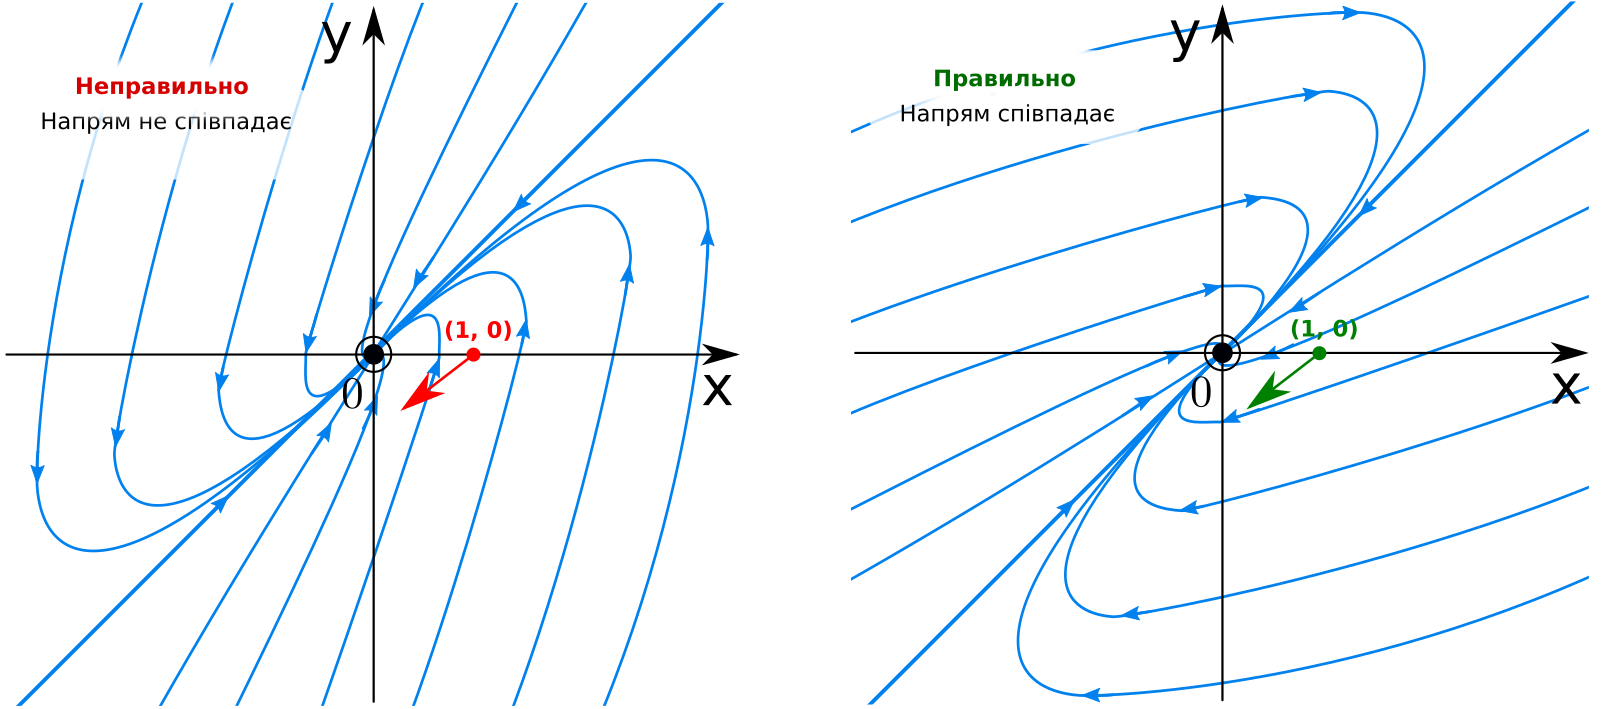
\includegraphics[scale=0.3]{assets/lectures_recent-f0de3cfc.png} \end{center}

Візьмемо т. (1, 0):
$$
\begin{bmatrix}
 \dot{x} \\
 \dot{y}
\end{bmatrix} \Bigg|_{(1,0)} = \begin{bmatrix}
 -3 \\
 -2
\end{bmatrix} \Longrightarrow \begin{gathered}
 x_k = -2 \\
 y_k = -2
\end{gathered}
$$

\end{example}

4. $\lambda_{1, 2} - \alpha \pm i\beta, \alpha\neq 0$. В такому випадку, фазовий портрет назвається \textbf{фокус}. Якщо $ \alpha > 0$ - нестійкий. Якщо $ \alpha > 0$ - ас. стійкий.
Фазовий портрет ''фокус'' може бути двох видів:
\begin{center} 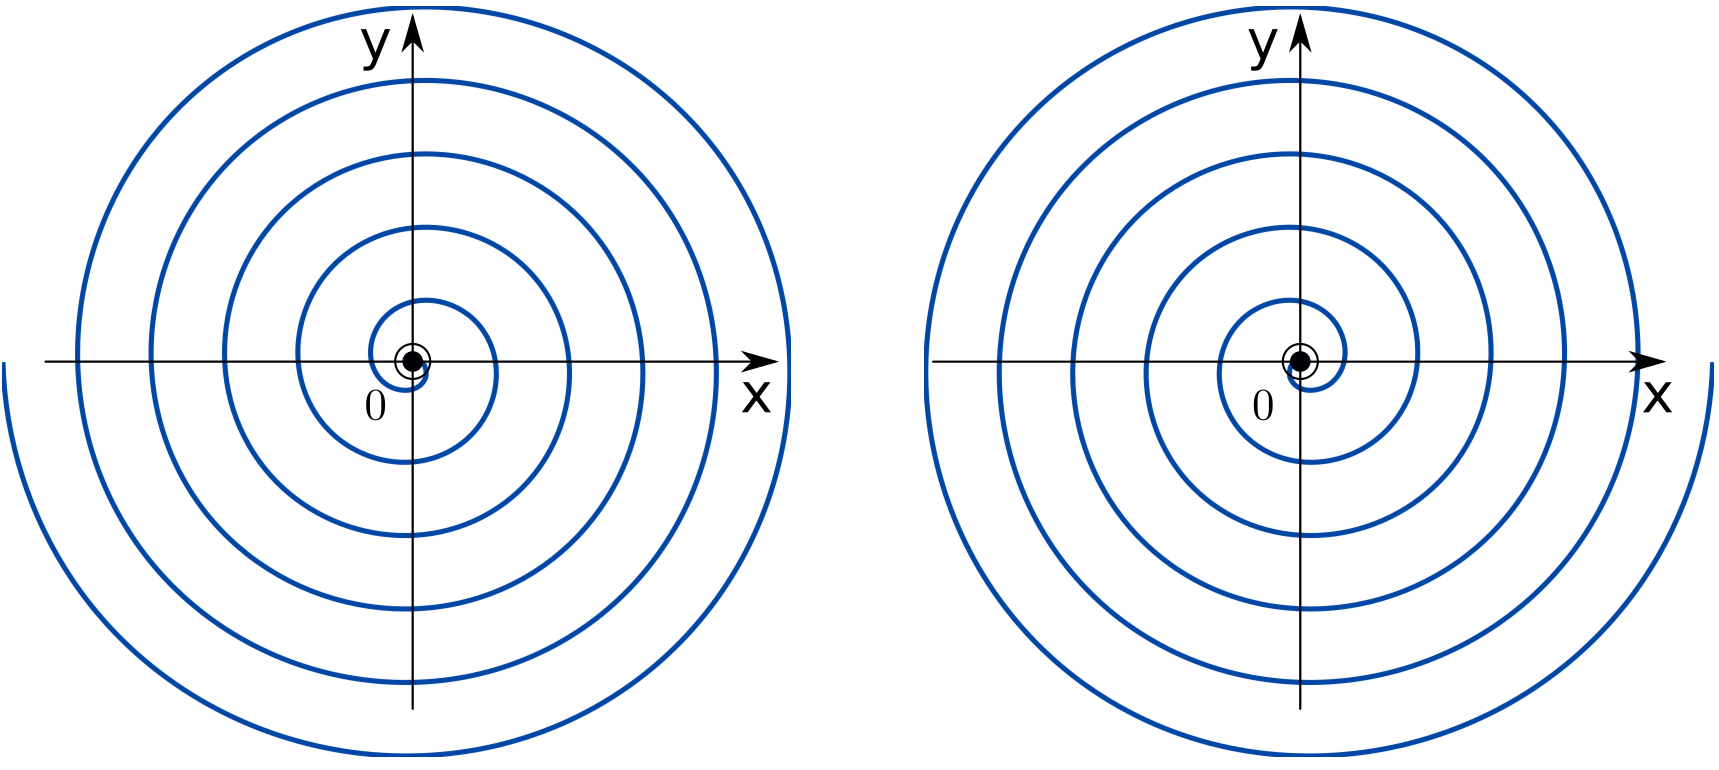
\includegraphics[scale=0.3]{assets/lectures_recent-9fe11a21.png} \end{center}
Для визначення типу фокуса визначаємо напрям вектора фазової швидкості в довільній точці, що не дорівнює нулю.

\begin{example}
    $$
    \begin{cases}
        \dot{x } = x - 2y\\
        \dot{y} = 4x - 3y
    \end{cases} \qquad A = \begin{bmatrix}
     1 & -2 \\
     4 & -3
    \end{bmatrix}
    $$
    $$ \det{(A - \lambda I)} = \begin{vmatrix}
      1- \lambda & -2 \\
      4 & -3-\lambda
    \end{vmatrix}  = ( 1- \lambda) (-3 - \lambda) + 8 = \lambda^2 + 2 \lambda + 5 = 0$$
$$
D = -16 \quad \lambda_{1,2} = \frac{-2 \pm 4i}{2} = -1 \pm 2i
$$
Асимптотично стійкий фокус (стрілки до нуля).
\begin{center} 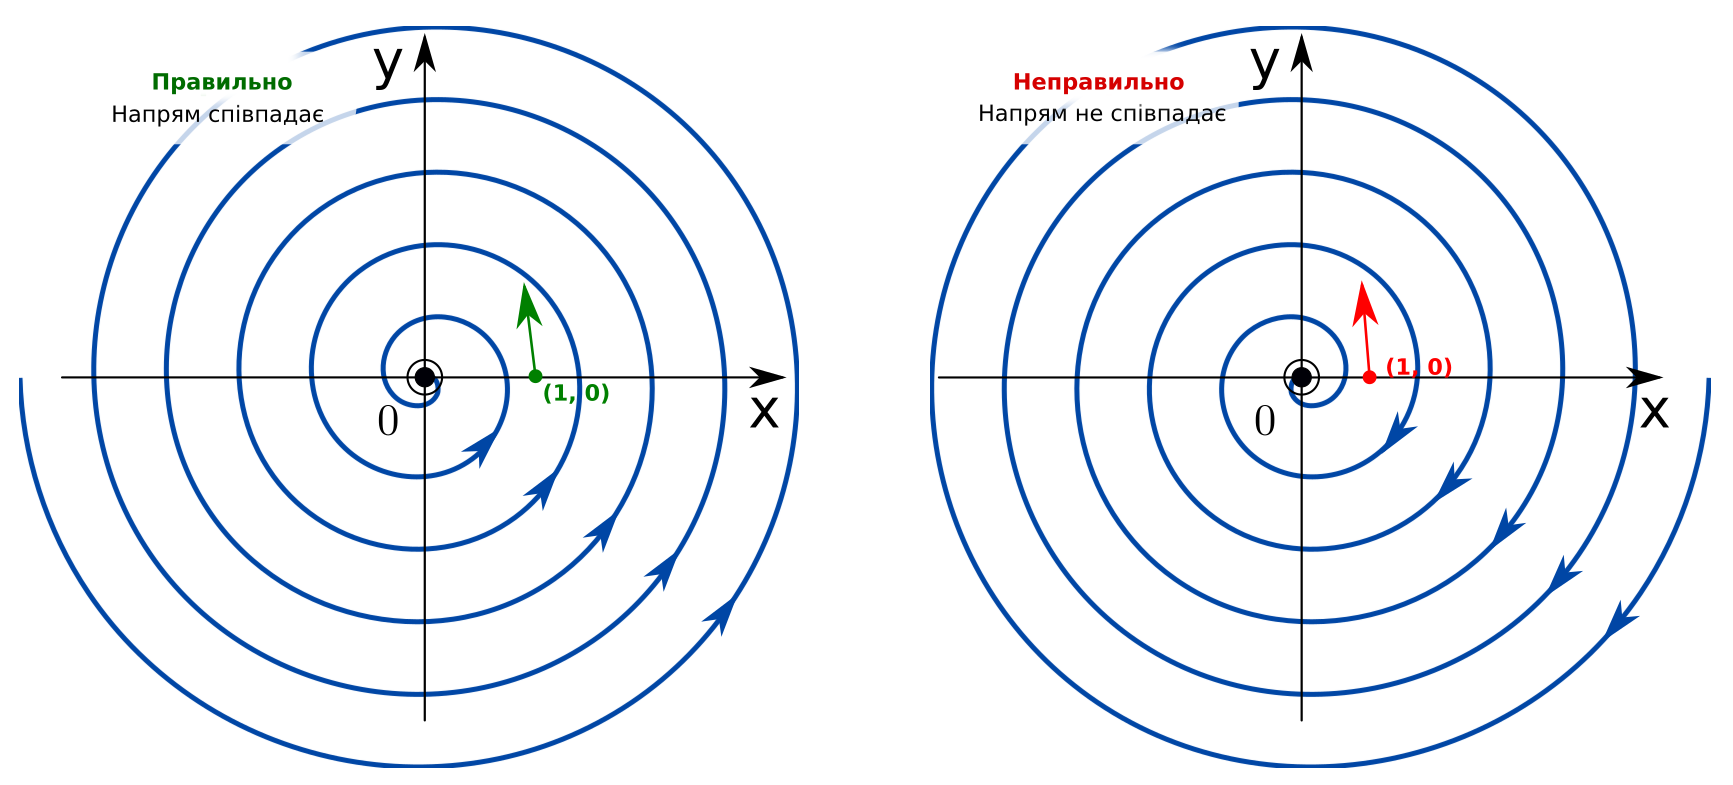
\includegraphics[scale=0.27]{assets/lectures_recent-b90426e3.png} \end{center}
Візьмемо точку (1, 0) для перевірки:

$$
\begin{bmatrix}
 \dot{x}\\
 \dot{y}
\end{bmatrix}\Bigg|_{(1,0)} - \begin{bmatrix}
 1 \\
 4
\end{bmatrix} \qquad \begin{gathered}
 x_k -1 = 1 \\
 y_k - 0 = 4
\end{gathered} \Rightarrow \begin{gathered}
 x_k = 2 \\
 y_k  = 4
\end{gathered}
$$
Отримали: $(1,0) \to (2, 4)$. Перевіримо за виглядом фазового портрета вище.
\end{example}

5.$ \lambda_{1,2} = \pm i \beta$. За таких власних чисел, фазовий портрет називається \textbf{центр.} (стійкий, але не асимптотично стійкий)
\begin{center} 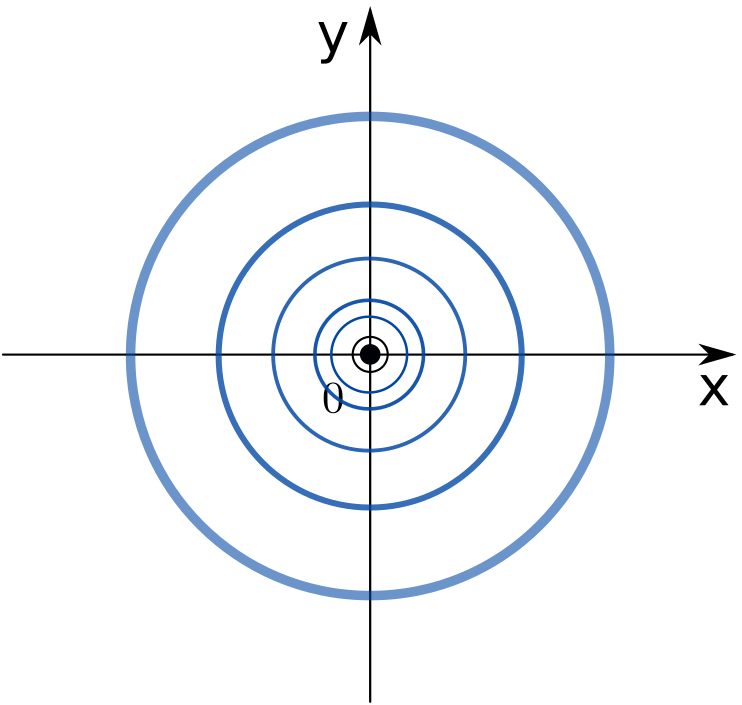
\includegraphics[scale=0.3]{assets/lectures_recent-2982f611.png} \end{center}

\begin{example}
    $$
    \begin{cases}
        \dot{x} = -2 x - 5y \\
        \dot{y} = 2x + 2y
    \end{cases} \qquad A = \begin{bmatrix}
     -2 & -5\\
     2 & 2
    \end{bmatrix}
    $$
    $$
    \det{(A - \lambda I)} = \begin{vmatrix}
      -2-\lambda & -5 \\
      2 & 2 -\lambda
    \end{vmatrix}  = \lambda^2 + 6 = 0 \Rightarrow \lambda = \pm i \sqrt{6} \Rightarrow \text{центр}
    $$
    Візьмемо т. (1, 0):
    $$
\begin{gathered}
\begin{bmatrix}
 \dot{x}\\
 \dot{y}
\end{bmatrix}\Bigg|_{(1,0)} = \begin{bmatrix}
 -2 \\
 2
\end{bmatrix} \\ \begin{cases}
  x_k -1 = -2\\
  y_k  - 0 = 2
\end{cases} \\
\begin{cases}
x_k = -1\\
    y_k  =2
\end{cases}
\end{gathered}\qquad    \begin{gathered} 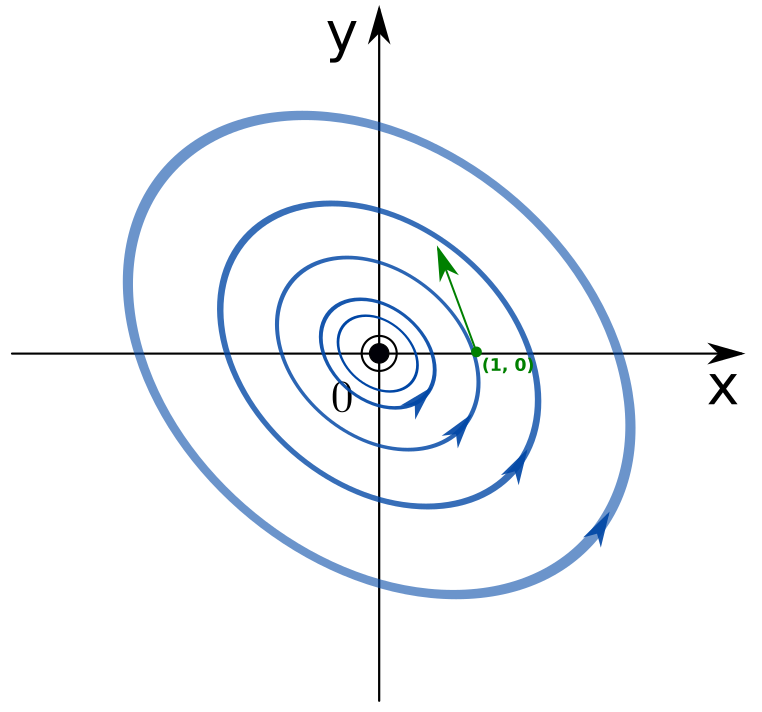
\includegraphics[scale=0.3]{assets/lectures_recent-1467e19e.png} \end{gathered}
    $$


\end{example}
6. Нехай $ \det A = 0$ (вирджений випадок).\\
$$
\det A  =  \begin{vmatrix}
  a & b\\
  c & d
\end{vmatrix} = ad - bc  = 0 \Rightarrow \frac{a}{c} = \frac{b}{d} = 0 \quad \begin{gathered}
 a = kc\\
 b = kd
\end{gathered}
$$
$$
\begin{cases}
    \dot{x} = ax+ by\\
    \dot{y} = k(ax + by)
\end{cases} \Rightarrow ax + by  = 0 \text{ - пряма положень рівноваги.}
$$

$$
\det ( A - \lambda I) = \begin{vmatrix}
  a - \lambda & b\\
  ka & kb - \lambda
\end{vmatrix} = (a-\lambda)*(kb- \lambda) - kab =
$$
$$
 = akb - a \lambda - kb \lambda +  \lambda^2 - kab = \lambda^2 - (a + kb) \lambda =0
 $$
 $$
 \lambda = 0 \qquad \lambda = a + bk
 $$

 a) Прямі паралельні власному вектору, що відповідає власному числу $\lambda =  a + bk$\\
 $\lambda > 0 $ - стрілки від нуля.\\
 $\lambda < 0 $ - стрілки до нуля.\\

 \begin{center} 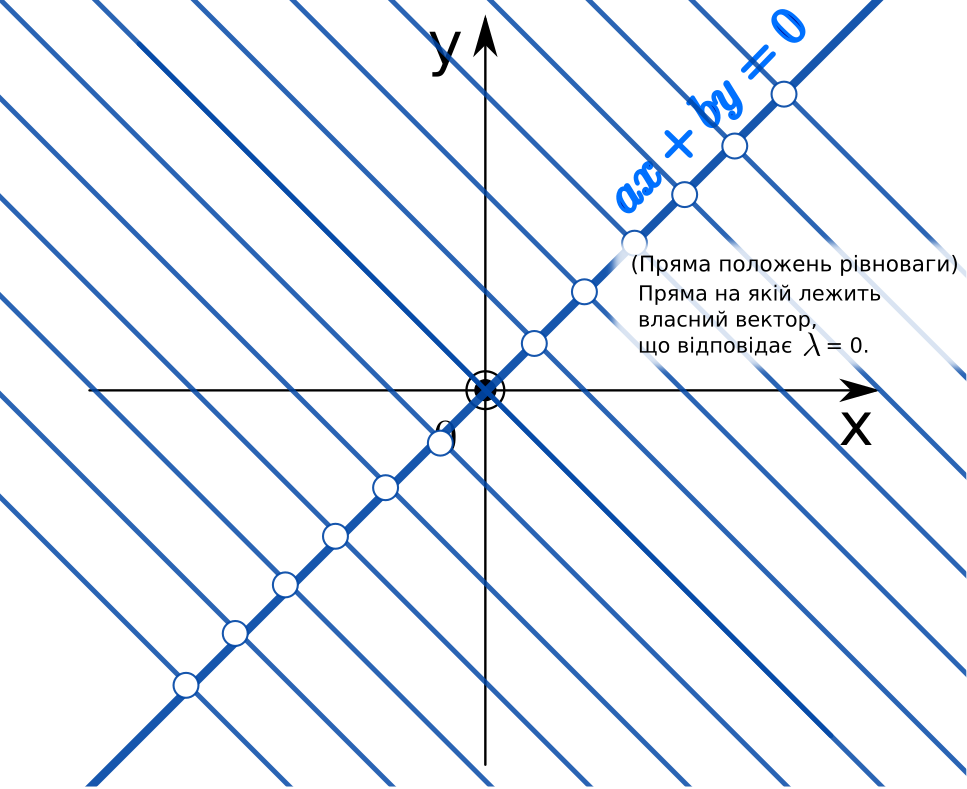
\includegraphics[scale=0.3]{assets/lectures_recent-058ceaff.png} \end{center}
b) $ \lambda_1 =  \lambda_2 = 0 \quad (a = - bk)$

\begin{center} 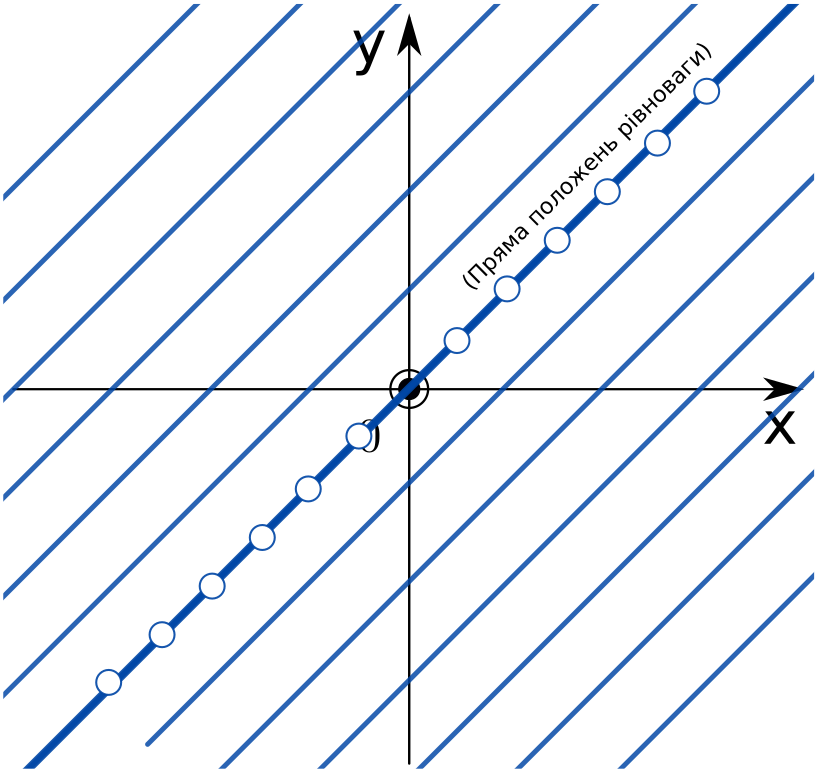
\includegraphics[scale=0.3]{assets/lectures_recent-49093f01.png} \end{center}

\end{document}
